% This must be in the first 5 lines to tell arXiv to use pdfLaTeX, which is strongly recommended.
\pdfoutput=1
% In particular, the hyperref package requires pdfLaTeX in order to break URLs across lines.

\documentclass[11pt]{article}

% Change "review" to "final" to generate the final (sometimes called camera-ready) version.
% Change to "preprint" to generate a non-anonymous version with page numbers.
% \usepackage[review]{acl}
\usepackage[final]{acl}

% Standard package includes
\usepackage{natbib}
\usepackage{xcolor}
\usepackage{hyperref}
\usepackage{times}
\usepackage{latexsym}
\usepackage{multirow}
\usepackage{multicol}
\usepackage{graphicx}
\usepackage{siunitx}
\usepackage{wrapfig}
\usepackage[most]{tcolorbox}
% For proper rendering and hyphenation of words containing Latin characters (including in bib files)
\usepackage[T1]{fontenc}
% For Vietnamese characters
% \usepackage[T5]{fontenc}
% See https://www.latex-project.org/help/documentation/encguide.pdf for other character sets

% This assumes your files are encoded as UTF8
\usepackage[utf8]{inputenc}

% This is not strictly necessary, and may be commented out,
% but it will improve the layout of the manuscript,
% and will typically save some space.
\usepackage{microtype}

% This is also not strictly necessary, and may be commented out.
% However, it will improve the aesthetics of text in
% the typewriter font.
\usepackage{inconsolata}

% This is also not strictly necessary, and may be commented out.
% However, it will improve the aesthetics of text in
% the typewriter font.
\usepackage{booktabs} % To thicken table lines
% For proper rendering and hyphenation of words containing Latin characters (including in bib files)
\usepackage{amsmath}
\usepackage{mathtools}
\usepackage{multirow}
\usepackage{siunitx}
\usepackage{lineno}
\usepackage{enumitem}
\usepackage{amsfonts}       % blackboard math symbols
\usepackage{nicefrac}       % compact symbols for 1/2, etc.
\usepackage{amsmath}
\usepackage{amssymb}
\usepackage[noend]{algpseudocode}
\usepackage{algorithm}
%\usepackage{algorithmic}
%\usepackage{algcompatible}
\usepackage{widebar}
\usepackage{subcaption}
\usepackage[textsize=scriptsize]{todonotes}
\usepackage{cuted}

% \usepackage{emoji}
\usepackage{array} % Required for custom column formatting

%%%%%%%%%%%%%%%%%%%%%%%%%%%%%%%%%%%%%%%%%%%%%%%%%%%%%%%%%%%%%%%%
%       ___          __   __                         __   __  
% |\ | |__  |  | __ /  ` /  \  |\/|  |\/|  /\  |\ | |  \ /__` 
% | \| |___ |/\|    \__, \__/  |  |  |  | /~~\ | \| |__/ .__/ 
%%%%%%%%%%%%%%%%%%%%%%%%%%%%%%%%%%%%%%%%%%%%%%%%%%%%%%%%%%%%%%%%

% If the title and author information does not fit in the area allocated, uncomment the following
%
%\setlength\titlebox{<dim>}
%
% and set <dim> to something 5cm or larger.

\definecolor{todoblue}{RGB}{33,150,243} % Define a custom color named "mycolor" as pure red

\definecolor{pink-color}{RGB}{255,1,97} 

\definecolor{red-color}{RGB}{255,111,105} 
\definecolor{dark-red-color}{RGB}{174,0,1} 
\definecolor{light-red-color}{RGB}{255,152,150} 


\definecolor{green-color}{RGB}{136,216,176} 
\definecolor{dark-green-color}{RGB}{49,163,84} 
\definecolor{light-green-color}{RGB}{136,216,176} 
\definecolor{sea-green-color}{RGB}{95,158,160} 

\definecolor{dark-blue-color}{RGB}{49,130,189} 
\definecolor{light-blue-color}{RGB}{158,202,225} 

\definecolor{grey-color}{RGB}{167,173,186}
\definecolor{dark-grey-color}{RGB}{79,91,102}
\definecolor{gold-color}{RGB}{247,205,15} 

\setlength{\fboxsep}{1.5pt}


\newcommand{\redtext}[1]{\textcolor{red-color}{#1}}
\newcommand{\redbg}[1]{\colorbox{red-color}{#1}}

\newcommand{\darkredtext}[1]{\textcolor{dark-red-color}{#1}}
\newcommand{\darkredbg}[1]{\colorbox{dark-red-color}{#1}}

\newcommand{\lightredtext}[1]{\textcolor{light-red-color}{#1}}
\newcommand{\lightredbg}[1]{\colorbox{light-red-color}{#1}}

\newcommand{\greentext}[1]{\textcolor{green-color}{#1}}
\newcommand{\greenbg}[1]{\colorbox{green-color}{#1}}

\newcommand{\darkgreentext}[1]{\textcolor{dark-green-color}{#1}}
\newcommand{\darkgreenbg}[1]{\colorbox{dark-green-color}{#1}}

\newcommand{\lightgreentext}[1]{\textcolor{light-green-color}{#1}}
\newcommand{\lightgreenbg}[1]{\colorbox{light-green-color}{#1}}

\newcommand{\darkbluetext}[1]{\textcolor{dark-blue-color}{#1}}
\newcommand{\darkbluebg}[1]{\colorbox{dark-blue-color}{#1}}

\newcommand{\lightbluetext}[1]{\textcolor{light-blue-color}{#1}}
\newcommand{\lightbluebg}[1]{\colorbox{light-blue-color}{#1}}


\newcommand{\greytext}[1]{\textcolor{grey-color}{#1}}
\newcommand{\greybg}[1]{\colorbox{grey-color}{#1}}

\newcommand{\goldtext}[1]{\textcolor{gold-color}{#1}}
\newcommand{\goldbg}[1]{\colorbox{gold-color}{#1}}


% \newcommand{\todo}[1]{\textcolor{todoblue}{#1}}

% If the title and author information does not fit in the area allocated, uncomment the following
%
%\setlength\titlebox{<dim>}
%
% and set <dim> to something 5cm or larger.
\newcommand{\ours}{\mbox{\textsc{SynthesizRR}}}
\newcommand{\oursshort}{\mbox{\textsc{SynthzRR}}}
\newcommand{\gold}{\mbox{\textsc{Gold}}}
\newcommand{\fewgen}{\mbox{\textsc{FewGen}}}
\newcommand{\retrgen}{\mbox{\textsc{RetrGen}}}

\newcommand{\Products}{\mbox{\textsc{Products}}}
\newcommand{\AmazonProducts}{\mbox{\textsc{Amazon Products}}}
\newcommand{\RealNews}{\mbox{\textsc{RealNews}}}

\newcommand{\RealNewsDominant}{\mbox{\textsc{RealNews/Dominant}}}
\newcommand{\RealNewsDom}{\mbox{\textsc{RealNews/Dom}}}
\newcommand{\RNDom}{\mbox{\textsc{RN/Dom}}}

\newcommand{\RealNewsRegional}{\mbox{\textsc{RealNews/Regional}}}
\newcommand{\RealNewsReg}{\mbox{\textsc{RealNews/Reg}}}
\newcommand{\RNReg}{\mbox{\textsc{RN/Reg}}}

\newcommand{\RealNewsIndia}{\mbox{\textsc{RealNews/India}}}
\newcommand{\RealNewsInd}{\mbox{\textsc{RealNews/Ind}}}
\newcommand{\RNInd}{\mbox{\textsc{RN/Ind}}}


\newcommand{\ToI}{\mbox{\textsc{ToI}}}
\newcommand{\TimesOfIndia}{\mbox{\textsc{Times of India}}}
\newcommand{\ToINews}{\mbox{\textsc{ToI News}}}
\newcommand{\Wiki}{\mbox{\textsc{Wiki}}}

\newcommand{\RetrICL}{\mbox{\textsc{Retr-ICL}}}
\newcommand{\NoRetrICL}{\mbox{\textsc{No-Retr-ICL}}}

\newcommand{\TinyBERT}{\mbox{\textsc{TinyBERT}}}
\newcommand{\DistilBERT}{\mbox{\textsc{DistilBERT}}}
\newcommand{\BERT}{\mbox{\textsc{BERT}}}
\newcommand{\DeBERTa}{\mbox{\textsc{DeBERTa-v3L}}}
\newcommand{\DeBERTaLarge}{\mbox{\textsc{DeBERTa-v3-Large}}}
\newcommand{\Cart}{\textsc{Cart}}
\newcommand{\GPTTwoXL}{\mbox{\textsc{GPT2-XL}}}
\newcommand{\ChatGPT}{\mbox{\textsc{GPT3.5-Turbo}}}
\newcommand{\ChatGPTShort}{\mbox{\textsc{GPT3.5-T}}}
\newcommand{\PhiMini}{\mbox{\textsc{Phi-3 Mini}}}
\newcommand{\Mixtral}{\mbox{\textsc{Mixtral}}}

\newcommand{\aref}[1]{\hyperref[#1]{Appendix~\ref*{#1}}}

\newcommand{\ZeroGen}{\textsc{ZeroGen}}
\newcommand{\ProGen}{\textsc{ProGen}}
\newcommand{\SunGen}{\textsc{SunGen}}
\newcommand{\ReGen}{\textsc{ReGen}}
\newcommand{\SynthesizRR}{\textsc{SynthesizRR}}
\newcommand{\LetsSynth}{\textsc{S3}}
\newcommand{\AttrPrompt}{\textsc{AttrPrompt}}
\newcommand{\AttrPromptShort}{\textsc{AttrPmt}}
\newcommand{\Human}{\textsc{Human}}


\newcommand{\dataxi}{\ensuremath{\mathbin{ x^{i}} }}
\newcommand{\dataxhat}{\ensuremath{\mathbin{ \tilde{x} }}}
\newcommand{\dataxihat}{\ensuremath{\mathbin{ \tilde{x}^{i}} }}
\newcommand{\icl}{ \mbox{in-context} learning}
\newcommand{\Icl}{\mbox{In-context} learning }
\newcommand{\rik}{\ensuremath{\mathbin{ R_k^{(i)}} }}
\newcommand{\datayi}{\ensuremath{\mathbin{ y^{i}} }}
\newcommand{\datayhat}{\ensuremath{\mathbin{ \check{y}} }}
\newcommand{\datayihat}{\ensuremath{\mathbin{ \check{y}^{i}} }}

\newcommand{\lm}{\ensuremath{\mathcal{M}_{\text{LM}}}}
\newcommand{\lmtask}{\ensuremath{ p_{\text{LM}}(x|y) }}

\newcommand{\studentlm}{\ensuremath{\mathcal{M}_{\text{S}}}}
\newcommand{\studentlmtask}{\ensuremath{ p_{\text{LM}}(y|x) }}

\newcommand{\clfdataset}{\ensuremath{\mathbin{
    \mathcal{D} = \{\dataxi, \datayi\}^{m}_{i=1}
}}}
\newcommand{\synthd}{\ensuremath{\mathbin{
    \mathcal{D}_{\textsc{Synth}}
}}}
\newcommand{\synthdataset}{\ensuremath{\mathbin{
    \synthd = \left\{ (\dataxihat, \datayi) \right\}^{m}_{i=1}
}}}

\newcommand{\winrate}[2]{\ensuremath{\mathbin{#1\text{:}#2}}}

\newcommand{\higherbetter}{\ensuremath{(\uparrow)}}
\newcommand{\lowerbetter}{\ensuremath{(\downarrow)}}

\newcommand{\higherbettersmall}{\scriptsize{\ensuremath{(\uparrow)}}}
\newcommand{\lowerbettersmall}{\scriptsize{\ensuremath{(\downarrow)}}}

\newcommand{\noeval}{\ensuremath{\footnotesize{\rotatebox[origin=c]{-90}{\hspace{-0.5ex}\otimes}}}}
\newcommand{\norelease}{\ensuremath{\scriptsize{\rotatebox[origin=c]{-90}{\hspace{-1ex}\bowtie}}}}

% \newcommand{\insection}[1]{\noindent\textbf{#1.}}
\newcommand{\insection}[2][.]{{\setlength{\parskip}{6pt} \noindent\textbf{#2#1}}}

\newcommand{\ignore}[1]{}
\newcommand{\ig}[1]{}

\newcommand{\paddedhline}{\vspace{1ex} \hline \vspace{-1ex}}
\newcommand{\promptsection}[1]{ 
\begin{center} \textbf{\underline{#1}} \end{center} \vspace{-2ex}
}
\newcommand{\promptsubsection}[1]{
\setlength{\parskip}{6pt} \noindent\textbf{{#1}:}
}
\newcommand{\param}[1]{
\textcolor{pink-color}{\scriptsize{\texttt{\detokenize{#1}}}}
}
\newcommand{\paramnorm}[1]{
\textcolor{pink-color}{\small{\texttt{\detokenize{#1}}}}
}
\newcommand{\prompttext}[1]{``\textcolor{dark-grey-color}{#1}''}
\newcommand{\verbal}[2]{
\textcolor{sea-green-color}{\detokenize{#1}}: ``\textcolor{dark-grey-color}{\detokenize{#2}}''
}


\newtcolorbox[list inside=prompt]{prompt}[1][]{
    colbacktitle=black!60,
    coltitle=white,
    fontupper=\footnotesize,
    boxsep=5pt,
    left=0pt,
    right=0pt,
    top=0pt,
    bottom=0pt,
    boxrule=1pt,
    title={Prompt~\thetcbcounter}, % Title format with auto counter
    #1,
}

\newcommand{\urlsmall}[1]{{\scriptsize{\url{\detokenize{#1}}}}}



%% Hide table columns: https://texblog.org/2014/10/24/removinghiding-a-column-in-a-latex-table/
\newcolumntype{h}{>{\setbox0=\hbox\bgroup}c<{\egroup}@{}}
%% Like p, but centers entire column horizontally while allowing width:
\newcolumntype{C}[1]{>{\centering\arraybackslash}m{#1}}
%% Like p, but right-aligns entire column horizontally while allowing width:
\newcolumntype{R}[1]{>{\raggedleft\arraybackslash}p{#1}}
%% Exactly like p...left-aligns entire column horizontally while allowing width:
\newcolumntype{L}[1]{>{\raggedright\arraybackslash}p{#1}}


%% Centers a single cell:
\newcommand{\cellhalign}[1]{\multicolumn{1}{c}{#1}}

\newcommand{\best}[1]{\textbf{#1}}
\newcommand{\tx}[1]{\mbox{\text{#1}}}

\newcommand{\incr}[1]{\mbox{\text{#1}}}
\newcommand{\decr}[1]{\mbox{\text{#1}}}


\newcommand{\LLaMa}{\mbox{\textsc{LLaMa2}}}
\newcommand{\LLaMaFull}{\mbox{\textsc{LLaMa-2 Chat 13B}}}
\newcommand{\Claude}{\mbox{\textsc{ClaudeV1}}}
\newcommand{\ClaudeFull}{\mbox{\textsc{Claude Instant-v1}}}

\newcommand{\IMDb}{\mbox{\textsc{IMDb}}}

\newcommand{\SST}{\mbox{\textsc{SST-2}}}

\newcommand{\Yelp}{\mbox{\textsc{Yelp}}}
\newcommand{\YelpPolarity}{\mbox{\textsc{Yelp Polarity}}}
\newcommand{\YelpDataset}{\mbox{\textsc{Yelp Dataset}}}
\newcommand{\YelpCorpus}{\mbox{\textsc{Yelp Businesses}}}
\newcommand{\YelpCorpusShort}{\mbox{\textsc{Yelp Biz.}}}


\newcommand{\CMUMovies}{\mbox{\textsc{CMU Movie Summary}}}
\newcommand{\CMUMoviesCorpus}{\mbox{\textsc{CMU Movie Summary}}}
\newcommand{\CMUMoviesCorpusShort}{\mbox{\textsc{CMU Movies}}}

\newcommand{\AGNews}{\mbox{\textsc{AG News}}}
\newcommand{\AG}{\mbox{\textsc{AG.}}}

\newcommand{\Hyperpartisan}{\mbox{\textsc{Hyperpartisan}}}
\newcommand{\HyperpartisanNews}{\mbox{\textsc{Hyperpartisan News}}}
\newcommand{\Hyper}{\mbox{\textsc{Hyper.}}}
\newcommand{\Hyp}{\mbox{\textsc{Hyp.}}}

\newcommand{\ToITopics}{\mbox{\textsc{ToI Topics}}}
\newcommand{\TimesOfIndiaTopics}{\mbox{\textsc{Times of India Topics}}}

\newcommand{\ToIHead}{\mbox{\textsc{ToI Head.}}}
\newcommand{\ToIHeadlines}{\mbox{\textsc{ToI Headlines}}}
\newcommand{\TimesOfIndiaHeadlines}{\mbox{\textsc{Times of India Headlines}}}

\newcommand{\ReviewCategory}{\textsc{Review Category}}
\newcommand{\AmazonReviewCategory}{\textsc{Amazon Review Category}}
\newcommand{\Category}{\mbox{\textsc{Category}}}
\newcommand{\Categ}{\mbox{\textsc{Categ.}}}
\newcommand{\Cat}{\mbox{\textsc{Cat.}}}

\newcommand{\QuestionHumor}{\mbox{\textsc{Question Humor}}}
\newcommand{\ProductQuestionHumor}{\textsc{Product Question Humor}}
\newcommand{\AmazonProductQuestionHumor}{\textsc{Amazon Product Question Humor}}
\newcommand{\Humor}{\mbox{\textsc{Humor}}}
\newcommand{\Intent}{\mbox{\textsc{Intent}}}
\newcommand{\Int}{\mbox{\textsc{Int.}}}
\newcommand{\Hum}{\mbox{\textsc{Hum.}}}

\newcommand{\ReviewPolarity}{\mbox{\textsc{Review Polarity}}}
\newcommand{\AmazonReviewPolarity}{\mbox{\textsc{Amazon Review Polarity}}}
\newcommand{\Polarity}{\mbox{\textsc{Polarity}}}
\newcommand{\Polar}{\mbox{\textsc{Polar.}}}
\newcommand{\Pol}{\mbox{\textsc{Pol.}}}

\newcommand{\BM}{\mbox{\textsc{BM25}}}
\newcommand{\Contriever}{\mbox{\textsc{Contriever}}}
\newcommand{\ContrieverShort}{\mbox{\textsc{Contr.}}}

\newcommand{\Reddit}{\mbox{\textsc{Reddit}}}
\newcommand{\StackExchange}{\mbox{\textsc{StackExchange}}}
\newcommand{\NYT}{\mbox{\textsc{NYT}}}


\DeclareMathOperator*{\bigplus}{\scalerel{+}}

\newcommand{\genex}[7]{
\begin{table*}[!t]
\centering
\tiny{
\setlength{\tabcolsep}{3pt}
\begin{tabular}{C{0.12\textwidth}p{0.84\textwidth}}
\toprule
\bf{Class} & \cellhalign{\bf{Example}} \\
\midrule
\textit{(Retrieved document)} & #3
\vspace{1.5ex}
\\ 
#2 & #4 \\
\midrule
\textit{(Retrieved document)} & #6
\vspace{1.5ex}
\\ 
#5 & #7 \\
\bottomrule
\end{tabular}
\vspace{-1ex}
}
\caption{
Generated examples for #1{} task using \ours{}.
}
\vspace{-3ex}
\end{table*}
}


\newtheorem{theorem}{Theorem}
\newtheorem{remark}{Remark}
\newcommand{\txb}[1]{\textcolor{blue}{#1}}
\newcommand{\txr}[1]{{\color{red}{#1}}}
\newcommand{\txg}[1]{{\color{green}{#1}}}
\newcommand{\distas}[1]{\mathbin{\overset{#1}{\kern0pt\sim}}}%
\def\corrsyn{{\textsc{CorrSynth}}}
\def\corrsynshort{{\textsc{CorrSyn}}}
\def\corrsynreallyshort{{\textsc{Corr}}}
\def\cC{\mathcal{C}}
\def\cX{\mathcal{X}}
\def\cY{\mathcal{Y}}
\def\cD{\mathcal{D}}
\def\cA{\mathcal{A}}
\def\cV{\mathcal{V}}
\def\cS{\mathcal{S}}
\def\cI{\mathcal{I}}
\def\cT{\mathcal{T}}
\def\eos{\mathtt{<eos>}}
\def\Prompt{\mathtt{prompt}}
\def\lg{\mathtt{lg}}
\def\mP{P}
\newcommand{\mbf}[1]{\mathbf{#1}}
\newcommand{\Pb}[1]{\mathbb{P}\left[#1 \right]}
\newcommand{\Pbx}[2]{\mathbb{P}_{#1}\left[#2 \right]}
\newcommand{\Ex}[1]{\mathbb{E}\left[#1 \right]}

% \newcommand\sk[1]{
% \todo[color=red!40]{
% \bf Suhas: #1
% }
% }
% \newcommand\vm[1]{
% \todo[color=green!40]{
% \bf Vijit: #1
% }
% }
% \newcommand\ad[1]{
% \todo[color=blue!40]{
% \bf Abhishek: #1
% }
% }

\newcommand\sk[1]{
% \todo[color=red!40]{\ig{
% \bf Suhas}: #1
% }
}
\newcommand\vm[1]{
% \todo[color=green!40]{\ig{
% \bf Vijit}: #1
% }
}
\newcommand\ad[1]{
% \todo[color=blue!40]{\ig{
% \bf Abhishek}: #1
% }
}



\title{CorrSynth - A Correlated Sampling Method for Diverse Dataset Generation from LLMs}

% Author information can be set in various styles:
% For several authors from the same institution:
% \author{Suhas S Kowshik\textsuperscript{1} \and Abhishek Divekar\textsuperscript{1} \and Vijit Malik \\
%         Amazon India}
% if the names do not fit well on one line use
%         Author 1 \\ {\bf Author 2} \\ ... \\ {\bf Author n} \\
% For authors from different institutions:
% \author{Author 1 \\ Address line \\  ... \\ Address line
%         \And  ... \And
%         Author n \\ Address line \\ ... \\ Address line}
% To start a separate ``row'' of authors use \AND, as in
% \author{Author 1 \\ Address line \\  ... \\ Address line
%         \AND
%         Author 2 \\ Address line \\ ... \\ Address line \And
%         Author 3 \\ Address line \\ ... \\ Address line}

% \author{First Author \\
%   Affiliation / Address line 1 \\
%   Affiliation / Address line 2 \\
%   Affiliation / Address line 3 \\
%   \texttt{email@domain} \\\And
%   Second Author \\
%   Affiliation / Address line 1 \\
%   Affiliation / Address line 2 \\
%   Affiliation / Address line 3 \\
%   \texttt{email@domain} \\}

%\author{
%  \textbf{First Author\textsuperscript{1}},
%  \textbf{Second Author\textsuperscript{1,2}},
%  \textbf{Third T. Author\textsuperscript{1}},
%  \textbf{Fourth Author\textsuperscript{1}},
%\\
%  \textbf{Fifth Author\textsuperscript{1,2}},
%  \textbf{Sixth Author\textsuperscript{1}},
%  \textbf{Seventh Author\textsuperscript{1}},
%  \textbf{Eighth Author \textsuperscript{1,2,3,4}},
%\\
%  \textbf{Ninth Author\textsuperscript{1}},
%  \textbf{Tenth Author\textsuperscript{1}},
%  \textbf{Eleventh E. Author\textsuperscript{1,2,3,4,5}},
%  \textbf{Twelfth Author\textsuperscript{1}},
%\\
%  \textbf{Thirteenth Author\textsuperscript{3}},
%  \textbf{Fourteenth F. Author\textsuperscript{2,4}},
%  \textbf{Fifteenth Author\textsuperscript{1}},
%  \textbf{Sixteenth Author\textsuperscript{1}},
%\\
%  \textbf{Seventeenth S. Author\textsuperscript{4,5}},
%  \textbf{Eighteenth Author\textsuperscript{3,4}},
%  \textbf{Nineteenth N. Author\textsuperscript{2,5}},
%  \textbf{Twentieth Author\textsuperscript{1}}
%\\
%\\
%  \textsuperscript{1}Affiliation 1,
%  \textsuperscript{2}Affiliation 2,
%  \textsuperscript{3}Affiliation 3,
%  \textsuperscript{4}Affiliation 4,
%  \textsuperscript{5}Affiliation 5
%\\
%  \small{
%    \textbf{Correspondence:} \href{mailto:email@domain}{email@domain}
%  }
%}

\makeatletter
\renewcommand{\@fnsymbol}[1]{\ifcase#1\or *\else\@arabic{#1}\fi}
\makeatother

\author{
\textbf{Suhas S Kowshik}\thanks{Equal contribution: order was determined by random dice rolls. Correspondence to: \texttt{adivekar@amazon.com}},
\textbf{Abhishek Divekar}\textsuperscript{*}, 
\textbf{Vijit Malik}
\\
Amazon
\\
\texttt{\{kowssuhp, adivekar, vijitvm\}@amazon.com}
}

\begin{document}
\maketitle


\begin{abstract}
% Large language models (LLMs) have demonstrated remarkable performance in diverse tasks using zero shot and few shot prompting. Even though their capabilities of data synthesis have been studied well in the recent years, the generated data suffers from lack of diversity, less adherence to the prompt and potential biases that creep into the data from the generator model. In this work, we tackle the challenge of generating datasets with high diversity, upon which when a student model is trained for down stream task. Taking the route of decoding time guidance based approaches, we propose \corrsyn{}, which generates data that is more diverse, and faithful to the input prompt using a correlated sampling strategy. Further our method overcomes the complexity drawbacks of some other guidance basd techniques like classifier based guidance. With extensive experiments, we show the effectiveness of our approach and substantiate our claims. In particular, we perform intrinsic evaluation to show the improvements to diversity. Our experiments show that \corrsyn{} improves both student metrics and intrinsic metrics upon competitive baselines across four datasets showing the innate advantage of our method.

Large language models (LLMs) have demonstrated remarkable performance in diverse tasks using zero-shot and few-shot prompting. Even though their capabilities of data synthesis have been studied well in recent years, the generated data suffers from a lack of diversity, less adherence to the prompt, and potential biases that creep into the data from the generator model. In this work, we tackle the challenge of generating datasets with high diversity, upon which a student model is trained for downstream tasks. Taking the route of decoding-time guidance-based approaches, we propose \corrsyn{}, which generates data that is more diverse and faithful to the input prompt using a correlated sampling strategy. Further, our method overcomes the complexity drawbacks of some other guidance-based techniques like classifier-based guidance. With extensive experiments, we show the effectiveness of our approach and substantiate our claims. In particular, we perform intrinsic evaluation to show the improvements in diversity. Our experiments show that \corrsyn{} improves both student metrics and intrinsic metrics upon competitive baselines across four datasets, showing the innate advantage of our method.
\end{abstract}
The advent of ChatGPT has significantly impacted both academia and industry due to its interactive capabilities and widespread application, establishing itself as a leading artificial intelligence tool \cite{DBLP:journals/corr/abs-2305-18486, DBLP:journals/corr/abs-2306-04504, DBLP:journals/corr/abs-2402-11203}. At the core of ChatGPT is the large language model (LLM) GPT-4, as detailed by \cite{achiam2023gpt}, which has seen numerous enhancements to its predecessors, showcasing exceptional abilities in a variety of Natural Language Processing (NLP) tasks \cite{DBLP:conf/ai/LaskarHH20}. Despite these advancements, the adoption of LLMs has highlighted several critical issues primarily due to their reliance on extensive datasets. This reliance restricts their ability to incorporate new information post-training, leading to three primary challenges. First, the focus on broad and general data to maximize accessibility and applicability results in subpar performance in specialized areas. Second, the rapid creation of online data, combined with the significant resources required for data annotation and model training, hinders LLMs' ability to stay updated. Third, LLMs are susceptible to generating convincing yet inaccurate responses, known as ``hallucinations'', which can mislead users.

\begin{figure}[t]
	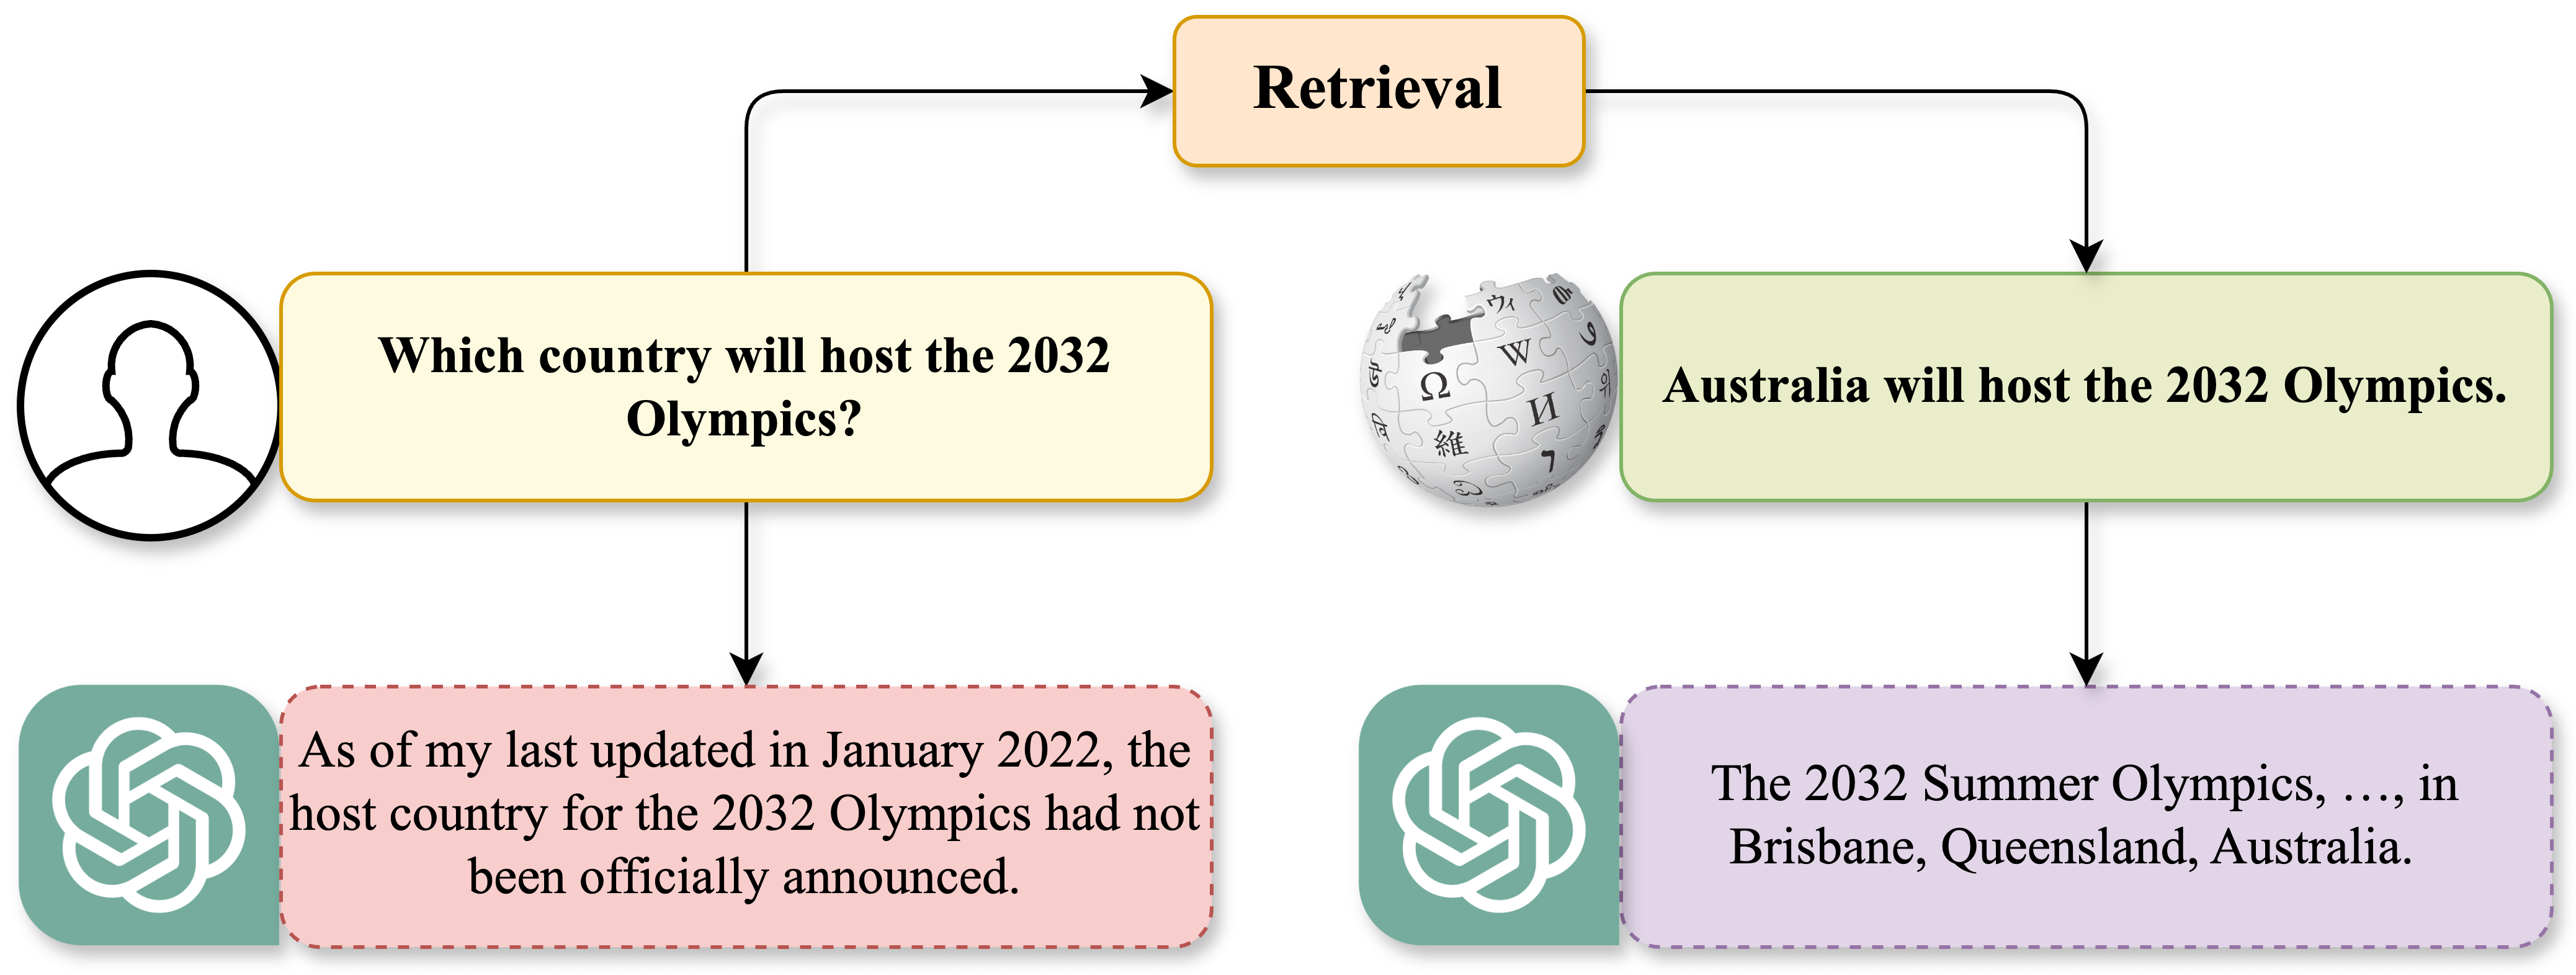
\includegraphics[width=0.6\textwidth]{Figures/RAG_example.png}
	\caption{An example of RAG benefits ChatGPT resolves questions that cannot be answered beyond the scope of the training data and generates correct results.}
	\label{fig:ragexample}
\end{figure}



Addressing these challenges is crucial for LLMs to be effectively utilized across various domains. A promising solution is the integration of Retrieval-Augmented Generation (RAG) technology, which supplements models by fetching external data in response to queries, thus ensuring more accurate and current outputs. Figure~\ref{fig:ragexample} illustrates how RAG can enable ChatGPT to provide precise answers beyond its initial training data.

Since its introduction by Lewis et al. \cite{lewis2020retrievalaugmented} in 2020, RAG has seen rapid development, especially with the rise of models like ChatGPT. Despite these advancements, there remains a noticeable gap in the literature regarding a comprehensive analysis of the mechanisms underlying RAG and the progress achieved by subsequent studies. Moreover, the field suffers from fragmented research focuses and inconsistent terminology for similar methods, leading to confusion. This survey seeks to bridge this gap by offering a structured overview of RAG, categorizing various approaches, and providing an in-depth understanding of the current research landscape, with a focus on textual applications given their prominence in recent research.

To provide clarity and structure, this paper is organized as follows: Section 2 outlines the overall RAG workflow, dividing the methodologies into pre-retrieval, retrieval, post-retrieval, and generation phases. Sections 3 through 6 explore the core techniques within each phase. Section 7 focuses on the evaluation methodologies for RAG. Section 8 summarizes the reviewed studies, detailing the retrievers and generators used, while Section 9 discusses challenges and future research directions, extending beyond text-based studies to include multimodal data applications. The paper concludes with Section 10.

Other related surveys provide valuable insights into the evolving RAG landscape from different angles. Gao et al. \cite{gao2023retrievalaugmented} identified three key stages in RAG development: pre-training enhancement, inference, and fine-tuning. Zhao et al. \cite{zhao2024retrievalaugmented} focused on the diverse applications of RAG, including text, code, image, and video generation, emphasizing augmented intelligence in generative tasks. Meanwhile, Hu et al. \cite{hu2024rau} explored Retrieval-Augmented Language Models (RALMs), examining how interactions between retrievers, language models, and augmentations influence model architectures and applications.

In this paper, we aim to offer a comprehensive and unified framework for understanding RAG from an information retrieval (IR) perspective, identifying key challenges and areas for improvement. We delve into the core technologies that drive RAG, assessing their effectiveness in addressing retrieval and generation tasks. Additionally, this survey introduces the evaluation methods employed in RAG research, highlights current limitations, and proposes promising avenues for future exploration.


\section{Background}
\label{sec:background}

% \paragraph{Notation:} Let $\mathbb{N}$ and $\mathbb{R}$ denote the sets of natural numbers and real numbers respectively. For $n\in\mathbb{N}$, let $[n]=\{1,2,\cdots,n\}$.\ad{This can be removed, not needed.} \ad{Makeit $P_{\theta}$ or $P_{\text{LM}}$ or $\mathcal{M}_{\text{LM}}(.)$, mention it is a teacher model}
\paragraph{Notation:} For $n\in\mathbb{N}$, let $[n]=\{1,2,\cdots,n\}$. An LLM is defined through its vocabulary $\cV$ and the auto-regressive sequence distribution $\mP$ or equivalently the logits $\lg$. Let $\cV^*=\cup_{n\geq 1}\cV^n$ denote the space of all finite sequences of tokens from $\cV$. We denote sequences of tokens from $\cV$ using lower boldface letters like $\mathbf{u},\mathbf{v}$. For any sequence of tokens $\mathbf{w}=(w_1,\cdots,w_n)\in \cV^n$ from $\cV$, and any $j\in[n]$, let $\mathbf{w}_{<j}=(w_1,\cdots,w_{j-1})$ if $j>1$, else, it is an empty sequence. Similarly $\mathbf{w}_{\leq j}=(w_1,\cdots,w_j)$. For any two sequences $\mathbf{u},\mathbf{v}\in\cV^*$ let $(\mathbf{u},\mathbf{v})$ denote their concatenation. We denote by $\mP(\mathbf{v}|\mathbf{u})$ the conditional probability of generating $(\mathbf{u},\mathbf{v})$ given that $\mathbf{u}$ has already been generated i.e., probability that $\mathbf{v}$ is a continuation of $\mathbf{u}$ for a given $\mathbf{u}$. Furthermore, for any $\mathbf{u},\mathbf{v}\in \cV^*$, we use $\mP(\cdot|\mathbf{u},\mathbf{v})$ to denote the conditioning on the concatenation $(\mathbf{u},\mathbf{v})$. For any prompt $\Prompt\in\cV^*$ , and any $\mathbf{w}\in\cV^n$, the auto-regressive distribution $\mP$ satisfies
\begin{align*}
    &\mP(\mathbf{w}|\Prompt)=\nonumber\\
    &\mP(w_1|\Prompt)\prod_{j=2}^{n}\mP(w_j|\Prompt,w_1,\cdots,w_{j-1})
\end{align*}
When we describe natural language domains using $\cX$, $\cY$ we mean either in the sense of them containing natural language sentences or as subsets of $\cV^*$, it will be clear from the context.%So $\mathbf{x}\in \cX$ can mean a piece of text, or its corresponding tokenization. The prompt for an LLM will be denoted by $\Prompt$ which can refer to the prompt text or its tokenization (i.e., an element of $\cV^*$).

We consider dataset generation for text classification tasks. Suppose we have a multiclass text classification problem with $K$ classes as $[K]$ and input domain $\cX$. Let $\cY=\{\mbf{y}_1,\cdots,\mbf{y}_K\}$ be the space of label verbalizations for the $K$ classes i.e., $\mbf{y}_k$ is a textual description of label $k\in[K]$. A natural language example input is denoted as $\mbf{x}\in\cX$. So the learning problem is defined on $\cX\times \cY$: given a data generating distribution $P_{XY}$ on $\cX\times \cY$ the task is to learn a classifier $h:\cX\to \cY$ (using some training data) such that $\Ex{l(h(\mbf{x}),\mbf{y})}$ is minimized for a given loss function $l:\cY\times\cY\to \mathbb{R}$, where the expectation is taken with respect to $P_{XY}$. 

Given the rapid advancement of LLMs like GPT-4, Llama2, Mistral etc. we are interested in utilizing the world knowledge and reasoning capabilities of these large models to generate synthetic training data for the textual $K$-class classification problem. Similar to recent works in this domain \cite{ye2022zerogen,gao2022self,Meng2022GeneratingTD,meng2023tuning,yu2023regen,ye2022progen,yu2024large,guo2024generative}, we consider the setup of prompting teacher LLM with a prompt $\Prompt$ that includes a label $\mbf{y}\in\cY$, a few In-Context Learning (ICL) examples for the label $\mbf{y}$ and potentially any other instance dependent attributes, and the prompt tasks the LLM to generate a synthetic instance $\mbf{x}\in \cX$ whose true label is expected to be $\mbf{y}$ i.e., the aim is to generate $x\distas{}P_{X|Y=\mbf{y}}$. That is, we generate a synthetic dataset \synthd{}. A student language model (e.g., a BERT-style pre-trained encoder model \citep{devlin-etal-2019-bert}) is trained on \synthd{}. 

For the ICL examples, we assume that we have access to a \emph{seed set} of examples $\mathcal{D}_{\textsc{Seed}} = \{(\mbf{x}_1,\mbf{y}_1),\ldots,(\mbf{x}_n,\mbf{y}_n)\}$. For us, typically $n$ is such that we have around $50$ examples per class.\sk{Abhishek, is this correct?} We assume that $\mathcal{D}_{\textsc{Seed}}$ is not large enough to train an effective student, but instead a larger synthetic dataset $\mathcal{D}_{\textsc{Synth}}=\{ (\tilde{\mbf{x}}_i,\mbf{y}_i)\}_{i=1}^m$  will be needed.% \synthdataset{}

A standard approach to dataset synthesis is few shot generation i.e. \fewgen{} \cite{NEURIPS2020_1457c0d6,ye2022progen,Yehudai2024GenieAH}. For instance, consider a task of detecting a business news article. In order to synthesize a dataset for this task, we could prompt the LLM appropriately, include few ICL examples. The LLM might generate a fairly decent article. But when we sample a large number of generations we see that the there is lack of diversity: similar entities are repeated, popular topics are highlighted and potential stylistic differences from a human written text. These could affect the performance of a student model that is trained on such dataset.

A ``good'' synthetic dataset must ensure that the conditional distribution of instances given any label must closely approximate that of the true distribution $P_{XY}$. This includes: i) correct semantic separation of labels, ii) preservation of intra-label semantic diversity and of course, iii) fluent and coherent generations. In order to achieve (i) and (ii) (without compromising on (iii)), we present a method, \corrsyn{}, in the flavor of decoding time guidance techniques \cite{li2023contrastive,o2023contrastive,sanchez2023stay,chuang2023dola}. In these works, at inference time, the token probability distribution is tilted by another distribution obtained either from a different LLM, or same LLM with a different prompt, or different layers of the same LLM. In particular, we take inspiration from the classifier free guidance~\cite{ho2021classifierfree} method applied to text based LLMs \cite{sanchez2023stay}. 
\corrsyn{} aims to control i) diversity in generations, ii) similarity to human crafted gold dataset, iii) cross label separation and at the same time iv) improve the student performance. The core idea of our approach is to perform correlated or dependent sampling from the LLM i.e., multiple sequences are generated in parallel that have strong dependency between each other. \autoref{fig:corrsynth_high_level} illustrates our method. More details are given in \autoref{sec:method}. This method can be used in conjunction with other synthetic dataset generation approaches like retrieval augmented generation~\cite{lewis2020retrieval}.


\begin{figure*}[t]
    \centering
    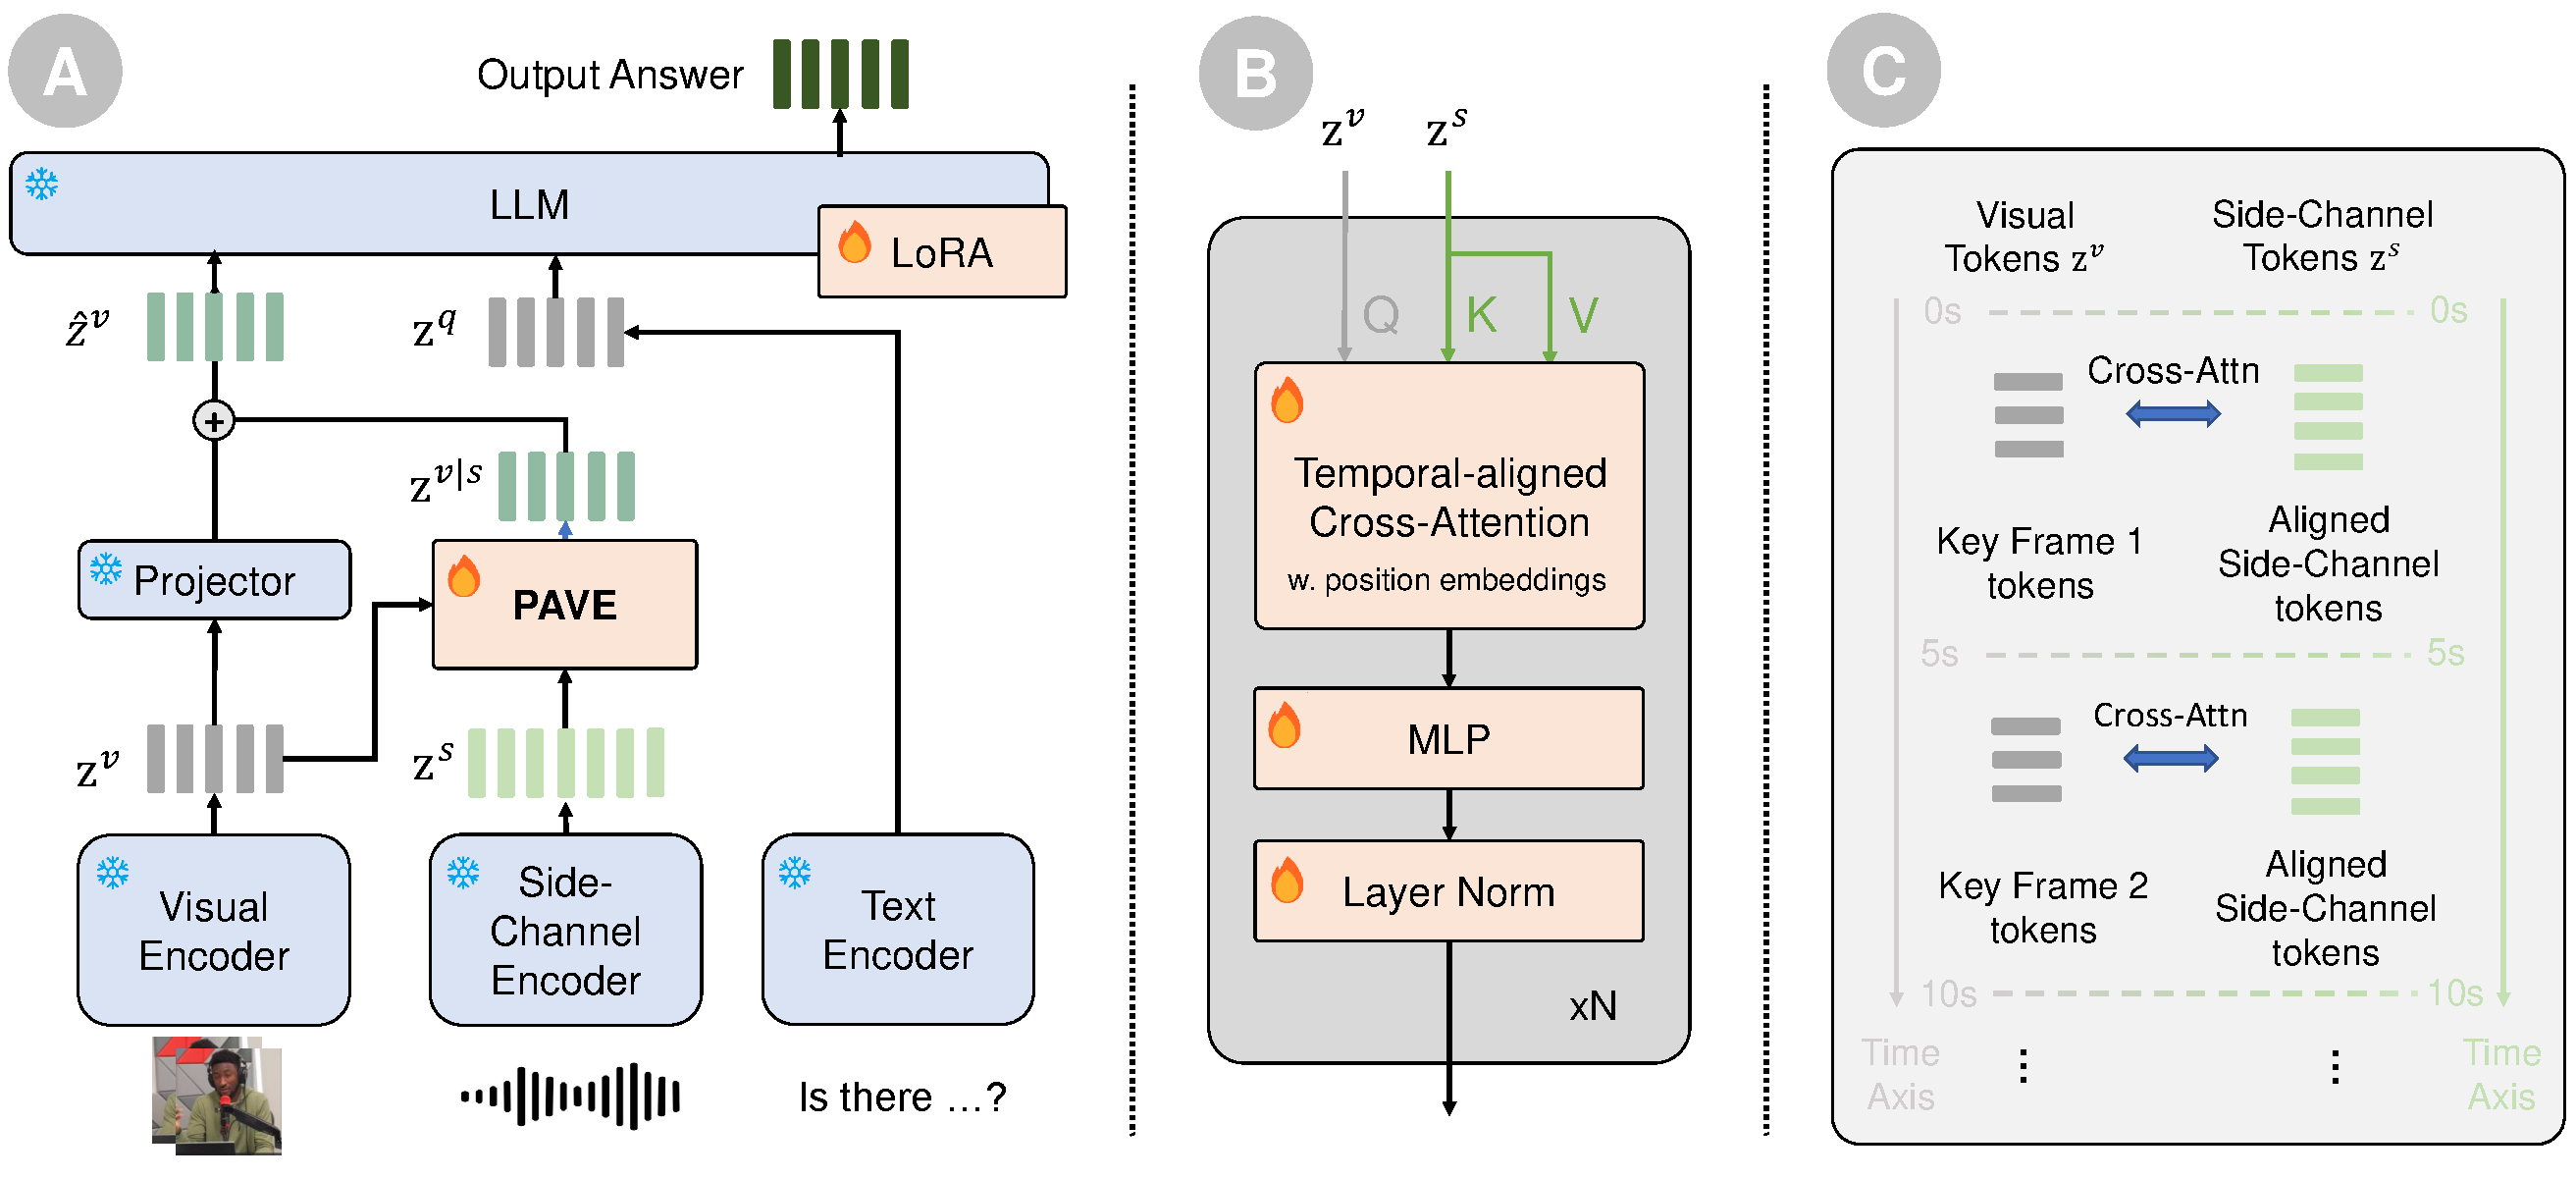
\includegraphics[width=0.85\linewidth]{new_figure_source/pave_overview_updated.pdf}
    \vspace{-0.5em}
    \caption{(a) \textbf{Overview of PAVE}. PAVE presents a simple, parameter-efficient adapter to integrate videos and side-channel signals. This is done by fusing side-channel tokens $\mathbf{z}^s$ and video tokens $\mathbf{z}^v$, and further adding the results to the original video tokens $\mathbf{z}^v$.  (b) \textbf{Details of PAVE's fusion function}. The fusion function $g(\cdot)$ consists of a few blocks of temporal-aligned cross-attention layer, MLP, and layer normalization. (c) \textbf{Temporal-aligned Cross-Attention}. Visual tokens $\mathbf{z}^v$ and side-channel tokens $\mathbf{z}^s$ are aligned along the temporal axis. A video token $\mathbf{z}^v(k)$ is treated as query, and only attends to keys and values (defined by side-channel tokens) in its temporal neighborhood.}
    \label{fig:structure_overview}
    \vspace{-1em}
\end{figure*}

\section{Patching and Adapting Video LLMs}
\label{sec:method}

% ovewview paragraph
We propose \textbf{PAVE}, a framework for adapting pre-trained Video LLMs to downstream tasks with side-channel signals. The key to our solution lies in a parameter-efficient, lightweight adapter, referred to as a patch. 
%only introduces a small number of parameters and operations and 
This patch fuses side-channel signals with the original visual tokens and updates them (see Figure~\ref{fig:structure_overview} (a)), and adds a LoRA module~\cite{hu2021loralowrankadaptationlarge} to the LLM, enabling efficient adaptation with a small number of parameters and operations and without altering the base model. 
%Additionally, we fine-tune the LLM using LoRA~\cite{hu2021loralowrankadaptationlarge}, enabling efficient adaptation through patching.
% ---
In what follows, we introduce the background on Video LLM, outline our problem formulation, and present our approach.
%and further describe the implementation details.   

%we present \textbf{PAVE}, a framework designed to \underline{P}atch and \underline{A}dapt \underline{V}id\underline{e}o LLMs. PAVE leverages a variant of cross-attention mechanism that operates between tokens derived from key video frames (as queries) and tokens from side-channel signals (as keys and values). This operations seeks to align the video frames and side-channel signals along the time axis, fuse the signals from both sources, and then update the input visual tokens to the LLM. In doing so, PAVE allows for the input of supplementary signals, and introduces a small number of parameters and operations with a negligible memory footprint and computing cost, while enabling effective adaptation to various downstream tasks without altering pre-trained models.


\subsection{Preliminaries: Video LLM}
A Video LLM takes a video $\mathbf{X}^v$ and a text query $\mathbf{X}^q=\{x^q\}$ as input, then generates a text answer $\mathbf{X}^a=\{x^a\}$. We assume that $\mathbf{X}^v = \{\mathbf{X}^v_1, \mathbf{X}^v_2, ..., \mathbf{X}^v_K\}$, \ie, a video is represented by $K$ key frames, where $K$ may vary across videos. $\mathbf{X}^v$ is first encoded by a visual encoder
% (including the vision backbone and its projector) 
$h_v(\cdot)$ into a set of visual tokens $\{\mathbf{z}^v(k) \in \mathbb{R}^{M \times d}\}$, where $\mathbf{z}^v(k)$ indicates $M$ tokens encoded from the $k$-th key frame within the video ($k \in [1, K]$). Similarly, $\mathbf{X}^q$ is processed by a text encoder $h_t(\cdot)$, which embeds individual words $x^q$ into text tokens $\{\mathbf{z}^q \in \mathbb{R}^d\}$ with $\mathbf{z}^q = h_t(x^q) $. 
These tokens are further combined and processed by an LLM $f(\cdot)$ that decodes $\mathbf{X}^a$ in an autoregressive manner
\begin{equation}
    f\left( \left[ \{\mathbf{z}^v(k)\}, \{\mathbf{z}^q\}, \{\mathbf{z}^a_{<i}\} \right]; \mathbf{\theta} \right) \rightarrow x_i^a, \label{eq:llm}
\end{equation}
where $\{\mathbf{z}^a_{<i}\}$ are text tokens from previously generated answer $x^a_{<i}$, \ie, $\mathbf{z}^a = h_t(x^a)$. $\mathbf{\theta}$ denotes LLM parameters. 

\subsection{Video Tasks with Side-Channel Signals}
% problem formulation / use cases
We consider adapting a pre-trained Video LLM to downstream tasks with side-channel signals $\mathbf{X}^s$. Similar to videos, we assume that $\mathbf{X}^s = \{\mathbf{X}^s_1, \mathbf{X}^s_2, ..., \mathbf{X}^s_{K_s}\}$, \ie, the side-channel signals also follow a temporal order and are split into $K_s$ blocks. We additionally assume a separate encoder (with possible projector) $h_s(\cdot)$ to process $\mathbf{X}^s$ into a collection of tokens $\{\mathbf{z}^s(k_s) \in \mathbb{R}^{M' \times d} \}$, where $\mathbf{z}^s(k_s)$ is $M'$ tokens encoded from the $k_s$-th block of the side-channel.  It is worth noting that this formulation encapsulates a range of video tasks. We describe some of these tasks considered in our experiments. 

\begin{itemize}
    \item \textbf{Audio-visual understanding}. This task requires jointly processing video and its accompanying audio data (as side-channel signals) for scene understanding, such as event recognition~\cite{xiao2020audiovisual} or QA~\cite{alamri2019audiovisualsceneawaredialog}. 
    \item \textbf{3D scene understanding}. This task focuses on reasoning about the 3D scene using a video of a 3D scan~\cite{azuma_2022_CVPR}. Camera trajectories, as well as an optional sequence of depth maps, constitute the side-channel signals.  
    \item \textbf{Multi-view video understanding}. This task involves combining multi-view videos for visual recognition, \eg, using exocentric videos to complement egocentric video for understanding human activities~\cite{grauman2024ego}. 
    \item \textbf{Enhancing video representations}. This task seeks to enhance the visual representation in the Video LLM. This is done by integrating low resolution, high frame rate frames with the original input of high resolution, low frame rate frames, following the key idea of SlowFast networks~\cite{feichtenhofer2019slowfastnetworksvideorecognition}.

\end{itemize}

\subsection{Our Design of PAVE}
% the key idea: x-attention for fusion and summation for aggregation; technical details about temporal alignment / positional encoding

Our goal is to integrate side-channel signals $\mathbf{X}^s$ into the LLM to enhance video reasoning, without modifying the structure of $f(\cdot)$ and encoders ($h_v(\cdot)$ and $h_t(\cdot)$), nor adding any major set of parameters. To achieve this goal, our key idea is learning a function $g(\cdot)$ to fuse side-channel tokens $\{\mathbf{z}^s(k_s)\}$ with the original visual tokens $\{\mathbf{z}^v(k)\}$. The fusion results have the same size of $\{\mathbf{z}^v(k)\}$, and will be further used to update $\{\mathbf{z}^v(k)\}$. Formally, our design of PAVE, as shown in Figure~\ref{fig:structure_overview} (a), is expressed as
\begin{equation}
\begin{split}
    \text{fusion:} \quad & \{\mathbf{z}^{v|s}(k)\} = g([\{\mathbf{z}^s(k_s)\}, \{\mathbf{z}^v(k)\}]; \phi)\\
    \text{summation:} \quad & \mathbf{\hat{z}}^{v}(k) = \mathbf{z}^{v}(k) + \mathbf{z}^{v|s}(k),
\end{split}\label{eq:pave}
\end{equation}
where $\phi$ denotes learnable parameters of $g(\cdot)$. 

Intuitively, $g(\cdot)$ injects side-channel information into a set of tokens of the same size as the original visual tokens, based on which a simple summation can be performed to form a residual connection. A key feature of this design is that the number of input tokens to $f(\cdot)$ remains unchanged. As the main computational cost lies in $f(\cdot)$, doing so results in a negligible overhead. 

\medskip
\noindent \textbf{The fusion function $g(\cdot)$}. Our fusion function is realized using a variant of cross-attention, as illustrated in Figure~\ref{fig:structure_overview} (b). Specifically, the vision tokens $\{\mathbf{z}^v(k)\}$ are transformed into the queries, and the side-channel tokens $\{\mathbf{z}^s(k_s)\}$ form the keys and values. To align video and side-channel signals in time while maintaining a low computation cost, we consider a local cross-attention, named temporal-aligned cross-attention, where a query $\mathbf{z}^v(k)$ only attends to keys and values in its temporal neighborhood, \ie, $\{\mathbf{z}^s(k_s)\}$ with $k_s \in N(k)$ (see Figure~\ref{fig:structure_overview} (c)). Before computing the cross attention, rotary positional embeddings~\cite{su2024roformer} are added to the queries and keys. After cross attention, an MLP with layer normalization is applied to further transform the features, similar to a standard Transformer block~\cite{vaswani2017attention}.


\medskip
\noindent \textbf{Integration with LoRA and training loss}. We further combine PAVE with LoRA~\cite{hu2021loralowrankadaptationlarge} by adding a small set of parameters in the form of low rank approximation $\Delta \theta$ to the LLM $f(\cdot)$. Putting things together, PAVE minimizes the standard negative log likelihood of its output when adapting to a downstream task. This is given by 
\begin{equation*}
\argmin_{\mathbf{\Delta\theta}, \mathbf{\phi}} \ \mathbb{E}_{\mathcal{D}} \ \left[ -\log p \left( x^a_i | \left[ \{\mathbf{\hat{z}}^{v}\}, \{\mathbf{z}^{q}\}, \{\mathbf{z}^a_{<i}\} \right]; \theta+\Delta \theta, \phi \right) \right],
\end{equation*}
where $\mathcal{D}$ is the data distribution approximated by the training set $(\mathbf{X}^v, \mathbf{X}^q, \mathbf{X}^a) \sim \mathcal{D}$. $\{\mathbf{\hat{z}}^{v}\}$ is computed using Eq.\ \ref{eq:pave}, thus creating a dependency on $g(\cdot)$ and its parameters $\phi$.
%The learnable parameters thus include the LoRA parameters $\Delta \theta$ in $f(\cdot)$, and the parameters $\phi$ in $g(\cdot)$ 

%A simple solution is given by LoRA~\cite{hu2021loralowrankadaptationlarge}. It learns a small set of parameters in the form of low rank approximation $\Delta \theta$. However, this solution does not allow us to make use of $\mathbf{X}^s$. 

% \subsection{Implementation Details}
% % all other things including some of the implementation details.
% Inside the attention layer, we add rotary position embedding to the query and key tokens. Specifically, we apply different rotary positional embedding according to the layout of side-channel tokens $\mathbf{z}^s$. We mainly consider two types of $\mathbf{z}^s$: (a) $\{\mathbf{z}^s\}$ includes both spatial and temporal dimensions, such as tokens from video backbones or from 3D backbone; and (b) $\{\mathbf{z}^s\}$ only contains temporal dimension, such as audio tokens. For the first case, we will add 3D rotary positional embedding (along the temporal, height, and width dimensions). For the second case, we will only add rotary positional embedding along the temporal axis. After cross-attention, we use a two-layer MLP, followed by a layer norm. We initialize the $\gamma$ in the layer norms to zero. For all experiments, we use a learning rate of 2e-5 and a batch size of 32 to adapt the pre-trained Video LLM.


\begin{comment}
\subsection{Background}
Current video Large Language Models (Video LLMs) have three components: Visual Encoder, Projector, and Language Model (LM).

\noindent\textbf{Visual Encoder.} It encodes the vision input into a latent feature space. The common choices for the vision encoder are ViT\cite{dosovitskiy2021imageworth16x16words} from CLIP\cite{radford2021learningtransferablevisualmodels}, SigLIP \cite{zhai2023sigmoidlosslanguageimage}, and multi-modality encoder LanguageBind\cite{zhu2023languagebind}. The encoded feature will be delivered to the adapter. We call features from the vision encoder as original visual tokens, $V_{origin}$.


\noindent\textbf{Projector.} The projector is the module convert the vision feature to the text latent space. In many recent research\cite{tong2024cambrian1fullyopenvisioncentric, liu2024llavanext} shows that the 2 layers MLP is strong enough to bridge the domain gap. We name the feature converted by after the projector as projected visual tokens, $V_{projectored}$

\noindent\textbf{Language Model.} The language model will process projected vision information and the questions to give an answer. The popular choice for the language model are Llama\cite{touvron2023llama2openfoundation,llama3_2}, Vicuna\cite{vicuna2023}, and Qwen-2\cite{yang2024qwen2technicalreport}.


\subsection{PAVE structure}
The overview of the PAVE structure is shown on the left panel of figure~\ref{fig:structure_overview}. For specific downstream tasks, the high level idea of PAVE is to create a 'Patch' and attach it to the Video LLM without altering the original model parameters and adapt the Video LLM into a new setting. This patch collects the task-specific additional information and add it back to the adapted visual tokens $V_{adapted}$, using a residual connection. 

\noindent\textbf{Input of the PAVE.} PAVE’s input has two sources: original visual tokens, $V_{origin}$, from the Video LLM's vision encoder, and the other is task-specific tokens $T$ from the encoder which encode the task-specific additional information.

\noindent\textbf{Temporal Alignment Module}
Given the fact that, the task-specific tokens $T$ and original visual tokens $V_{origin}$ may have different temporal granularities. Considering that temporally close visual and additional information are strongly correlated, as they jointly represent the same scene, we use temporal alignment module to explicit align them. This approach not only reduces noise introduced by temporal misalignment but also further reduces computational resource needed in cross-attention.

To do this we first split the task-specific tokens $T$ and original visual tokens $V_{origin}$ based on their smallest temporal unit, respectively. We then have $T = \{T_0, T_1, ... , T_n\}$ and $V_{origin}=\{V_0, V_1, ... , V_m\}$. For instance, if input of the Video LLM's vision encoder consist of 32 frames, then original visual tokens $V_{origin}$ should be split into $\{V_0, V_1, ... , V_{31}\}$. We always use the $\{V_0, V_1, ... , V_m\}$ as anchors on the temporal axis and evenly divide the $\{T_0, T_1, ... , T_n\}$ into $m$ groups.


\begin{align*}
\{T_0, T_1, \dots, T_n\} &= \Big\{ \{T_{00}, T_{01}, \dots, T_{0k}\}, \\ 
                          &\quad \{T_{10}, T_{11}, \dots, T_{1k}\}, \dots, \\ 
                          &\quad \{T_{m0}, T_{m1}, \dots, T_{mk}\} \Big\}
\end{align*}


For some special case that $\{T_0, T_1, ... , T_n\}$ could not be evenly split into m groups, we will pad the group which lengthen is smaller than $\ceil*{\frac{n}{m}}$. Right panel of figure~\ref{fig:structure_overview} show the visualization of temporal alignment module. We then pair the $V_i$ with $\{T_{i0}, T_{i1}, \dots, T_{ik}\}$ as mini-batch $mbatch_i = (V_i, \{T_{i0}, T_{i1}, \dots, T_{ik}\})$ and create $m$ mini-batches in total.

\noindent\textbf{Cross-Attention Module and 3-dimension Rotary Positional Embedding.}
After Obtaining the $m$ mini-batches from the Temporal Alignment Module we conduct cross-attention within each mini-batch, Where $V_i$ will be the query and $\{T_{i0}, T_{i1}, \dots, T_{ik}\}$ will be the key. Thus it aggregate the additional information from $\{T_{i0}, T_{i1}, \dots, T_{ik}\}$ into $V_i$ and and yield a group of updated tokens $V_{updated}=\{V_{updated_0}, V_{updated_1}, ... , V_{updated_m}\}$

During the cross-attention, We mainly consider two types of task-specific tokens $T$ : 1. tokens $T$ with spatial dimensions, such as video tokens from video backbones and 3D tokens from 3D backbone, 2. tokens $T$ without spatial dimensions, such as audio tokens. For the first case we will add 3 dimension rotary positional embedding along the temporal, height and width dimension. For the second case we will only add rotary positional embedding along the temporal axis.

\noindent\textbf{Zero-Initialized Residual Connection.}  After aggregating all additional information into $V_{updated}$, $V_{updated}$ will pass through an MLP and a Layer Normalization layer. Specifically, we initialize the $\gamma$ in layer norm to zero, this will ensure that the beginning of the training PAVE module will not have any effect on the Video LLM. 
Finally we add up $V_{updated}$ with the projected visual tokens $V_{projected}$. The $V_{adaptored} = V_{updated} + V_{projected}$ will be sent into the LLM for reasoning.

\subsection{The Training of PAVE}
In the PAVE, the Cross-Attention layers, the MLP and the layer normalization layer are trainable, while other modules remain forzen. During the adaptation, we also apply LoRA to the LLM to adapt the LLM for making use of the additional information.
We use the original auto-regressive training objective to train the PAVE, specially for a sequence of length L, we maximize the probability of the target answers $\mathbf{X}_\text{a}$ during the adaptation by:
\begin{align*}
        p(\mathbf{X}_\text{a} \mid V_{adaptored}, \mathbf{X}_\text{instruct}) = \\
    \prod_{i=1}^{L} p_\theta (x_i \mid V_{adaptored}, \mathbf{X}_\text{instruct, $<$ i}, \mathbf{X}_\text{a, $<$ i})
\end{align*}
where, the $\mathbf{X}_\text{a}$ is the target answer, $V_{adaptored}$ is the PAVE adapted visual features, $\mathbf{X}_\text{instruct}$ is the question and instruction, and $\theta$ represent the all trainable parameters.
\end{comment}
\section{Experimental Setup}
\label{sec:expt-setup}


 % Please add the following required packages to your document preamble:
% \usepackage{booktabs}
\begin{table}
\small
\centering
\begin{tabular}{@{}lccc@{}}
\toprule
\textbf{Dataset} & \textbf{Type} & \textbf{Class} & \textbf{Train, Test} \\ 
\midrule
\AGNews   & Topic            & $4$              & $115\text{K}, 7.6\text{K}$           \\
\ToIHeadlines   & Topic            & $10$             & $52\text{K}, 10\text{K}$             \\
\Humor   & Sentiment      & $2$     & $15\text{K}, 3\text{K}$   \\
\IMDb   & Sentiment      & $2$     & $20\text{K}, 25\text{K}$   \\ 
\bottomrule
\end{tabular}
\caption{Dataset statistics.}
\vspace{-1em}
\label{tab:tasks}
\end{table}


% \begin{table}
% \small
% \centering
% \setlength{\tabcolsep}{3pt}
% \begin{tabular}{
% l
% c
% c
% c
% h
% }
% \toprule
% \textbf{Corpus} & \textbf{Domain} & \textbf{Docs} & \textbf{Item} & \textbf{Tokens} \\ \midrule

% \RealNewsDom    & US/EU News    & $30.1\text{M}$   & News article     & $27.1\text{B}$ \\
% % \RealNewsReg    & Regional News     & $2.7\text{M}$    & Article     & $2.1\text{B}$ \\
% \textsc{\RealNewsInd}  & Indian News     & $0.9\text{M}$    & News article     & $0.6\text{B}$ \\
% \Products   & E-commerce        & $15.0\text{M}$   & Product   & $2.3\text{B}$ \\
% \YelpCorpus   & Commerce        & $150\text{K}$   & Business  & $2.3\text{B}$ \\
% \CMUMoviesCorpusShort   & Movies        & $42\text{K}$   & Movie plot   & $2.3\text{B}$ \\

% \bottomrule
% \end{tabular}
% \caption{
% Corpus statistics. 
% % \vm{Need to add train test sizes for yelp and imdb in the table}
% }
% \label{tab:corpus}
% \end{table}

\paragraph{Datasets.} \ad{Remove and cut down} We experiment on 4 datasets described in \autoref{tab:tasks}, which are selected to encompass a wide scope of generation tasks (news headlines, news articles, humorous product questions and movie reviews). Previous work primarily benchmarked only sentiment and topic classification datasets. We consider: (1) \AGNews{}~\citep{zhang2015character}, a popular topic classification dataset where each news summary is mapped to a news topic. The generation task involves generating news summaries based on news topics; (2) \ToIHeadlines{}\cite{toiheadlines}, similarly is a topic classification dataset of regional news headlines in India that maps news topics to news headlines; the generation task is similar to \AGNews{}. The difficulty is that the headlines is regionalized to Indian news and hence requires India specific entities; (3) \Humor~\citep{humor} task involves generating humorous and non-humorous questions from retrieved product details; (4) \IMDb{} \cite{maas-etal-2011-learning} is a sentiment task with binary labels. Prompts are in \autoref{app:prompts}.


% Please add the following required packages to your document preamble:
% \usepackage{booktabs}
% \usepackage{multirow}
\begin{table*}[h]
\centering
\begin{tabular}{
L{65pt}
% h
c % Teacher
C{16pt} % AG 
C{17pt} % ToI
C{18pt} % Humor
C{24pt} % IMDb
C{20pt} % Avg
|C{16pt} % AG 
C{17pt} % ToI
C{18pt} % Humor
C{24pt} % IMDb
C{20pt} % Avg
}

\toprule
\multirow{2}{*}{\textbf{Method}}   
& \multirow{2}{*}{\textbf{Teacher}} %\multicolumn{1}{h}{\multirow{2}{*}{\textbf{Params}}}
% &  %\multicolumn{1}{C{26pt}}{\multirow{2}{*}{\textbf{Teacher}}}
& \multicolumn{4}{c}{\textbf{Accuracy \higherbetter}}
& \multirow{2}{*}{\textbf{Avg.}}
& \multicolumn{4}{c}{\textbf{MAUVE \higherbetter}}
& \multirow{2}{*}{\textbf{Avg.}}
\\ 
\cmidrule(l){3-6}         
\cmidrule(l){8-11}         
% & 
& \textbf{LM} % \multicolumn{1}{c}{\textbf{LM}}
& \textbf{\AG} % AG Accuracy
& \textbf{\ToI} % ToI Accuracy
& \textbf{\Hum} % Hum Accuracy
& \textbf{\IMDb} % IMDb Accuracy
&
& \textbf{\AG} % AG Mauve
& \textbf{\ToI} % ToI Mauve
& \textbf{\Hum} % Hum Mauve
& \textbf{\IMDb} % IMDb Mauve
&
\\ 
\midrule
\gold          
% & %\multicolumn{1}{c}{-}                
& \multicolumn{1}{c}{-}                
& 91.4         & 78.9         & 92.9          & 91.4 & 88.7
& -         & -         & -          & - & -
\\ 
\midrule
%% Few-shot (Human seed)
\multicolumn{12}{c}{\underline{\textsc{In-Context Learning}}} \\
[0.5ex]
\fewgen 
% & % \multicolumn{1}{c}{-} 
& \multicolumn{1}{c}{\PhiMini}          
& 83.8         & 69.7         & 68.5          & 85.1 & 76.8
& 91.0         & 86.3        & 83.7          & 67.7 & 82.2
\\ 
\fewgen 
% & % \multicolumn{1}{c}{-} 
& \multicolumn{1}{c}{\Mixtral}          
& 72.3         & 47.3         & 82.8          & 87.1 & 67.5
& 87.1         & 91.6         & 87.0          & 64.6 & 82.6
\\ 
[1.0ex]

\corrsynreallyshort-Intra 
% & % \multicolumn{1}{c}{-} 
& \multicolumn{1}{c}{\PhiMini}          
& 84.8         & 71.0         & 84.7          & 87.1 & 81.9
& 82.3         & 83.2         & 82.3          & 77.4 & 81.3
\\ 
\corrsynreallyshort-Hybrid 
% & % \multicolumn{1}{c}{-} 
& \multicolumn{1}{c}{\PhiMini}          
& \textbf{85.1}         & \textbf{71.1}         & 85.1          & 86.8 & \textbf{82.1}
& 77.5         & 82.0         & 81.7          & 71.0 & 78.1
\\ 
[0.5ex]

\corrsynreallyshort-Intra 
% & % \multicolumn{1}{c}{-} 
& \multicolumn{1}{c}{\Mixtral}
& 78.5         & 68.9         & \textbf{86.5}          & \textbf{88.6} & 80.1
& \textbf{94.4}         & 95.6         & 95.5          & 76.8 & 90.1
\\  
\corrsynreallyshort-Hybrid 
% & % \multicolumn{1}{c}{-} 
& \multicolumn{1}{c}{\Mixtral}
& 73.6         & 68.4         & 86.0          & 88.1 & 79.0
& 93.8         & \textbf{96.1}         & \textbf{97.1}          & \textbf{80.5} & \textbf{91.9}
\\ 
[1.0ex]
\toprule
\multirow{2}{*}{\textbf{Method}}   
& \multirow{2}{*}{\textbf{Teacher}} %\multicolumn{1}{h}{\multirow{2}{*}{\textbf{Params}}}
% &  %\multicolumn{1}{C{26pt}}{\multirow{2}{*}{\textbf{Teacher}}}
& \multicolumn{4}{c}{\textbf{Self-BLEU-5 \lowerbetter}}
& \multirow{2}{*}{\textbf{Avg.}}
& \multicolumn{4}{c}{\textbf{Entity-Entropy \higherbetter}}     
& \multirow{2}{*}{\textbf{Avg.}}
\\
\cmidrule(l){3-6}         
\cmidrule(l){8-11}         
% & 
& \textbf{LM} % \multicolumn{1}{c}{\textbf{LM}}
& \textbf{\AG} % AG Accuracy
& \textbf{\ToI} % ToI Accuracy
& \textbf{\Hum} % Hum Accuracy
& \textbf{\IMDb} % IMDb Accuracy
&
& \textbf{\AG} % AG Mauve
& \textbf{\ToI} % ToI Mauve
& \textbf{\Hum} % Hum Mauve
& \textbf{\IMDb} % IMDb Mauve
&
\\
\midrule
\gold          
% & %\multicolumn{1}{c}{-}                
& \multicolumn{1}{c}{-}                
& 17.1         & 7.9         & 19.8          & 27.9 & 18.2
& 6.6         & 6.1         & 5.1          & 7.5 & 6.3
\\ 
\midrule
\multicolumn{12}{c}{\underline{\textsc{In-Context Learning}}} \\
[0.5ex]
\fewgen 
% & % \multicolumn{1}{c}{-} 
& \multicolumn{1}{c}{\PhiMini}          
& 33.9         & 15.3         & 39.9          & 57.7 & 36.7
& 6.6         & 6.3         & 4.3          & 5.3 & 5.6
\\ 
\fewgen 
% & % \multicolumn{1}{c}{-} 
& \multicolumn{1}{c}{\Mixtral}          
& 39.4         & 37.9         & 64.6          & 66.5 & 52.1
& 5.9         & 5.2         & 3.6         & 5.2 & 5.0
\\ 
[1.0ex]
% \oursshort & \multicolumn{1}{c}{-}  & \multicolumn{1}{c}{\PhiMini}          
% & 91.3         & 94.5         & 91.4          & 91.4
% & 91.3         & 94.5         & 91.4          & 91.4
% \\ 
% \oursshort & \multicolumn{1}{c}{-} & \multicolumn{1}{c}{\Mixtral}          
% & 91.3         & 94.5         & 91.4          & 91.4
% & 91.3         & 94.5         & 91.4          & 91.4
% \\ 
% [0.5ex]
% \corrsynreallyshort-Cross 
% % & % \multicolumn{1}{c}{-} 
% & \multicolumn{1}{c}{\PhiMini}          
% & 91.3         & 94.5         & 91.4          & 91.4 & -
% & 91.3         & 94.5         & 91.4          & 91.4 & -
% \\ 
\corrsynreallyshort-Intra 
% & % \multicolumn{1}{c}{-} 
& \multicolumn{1}{c}{\PhiMini}          
& 13.1         & 9.0         & 23.5          & 24.9 & 17.6
& \textbf{7.4}         & \textbf{6.9}         & \textbf{4.9}          & \textbf{6.5} & \textbf{6.4}
\\ 
\corrsynreallyshort-Hybrid 
% & % \multicolumn{1}{c}{-} 
& \multicolumn{1}{c}{\PhiMini}          
& \textbf{12.1}         & \textbf{8.7}         & \textbf{22.8}          & \textbf{19.2} & \textbf{15.7}
& \textbf{7.4}         & \textbf{6.9}        & 4.8          & 6.4 & \textbf{6.4}
\\ 
[0.5ex]
% \corrsynreallyshort-Cross 
% % & % \multicolumn{1}{c}{-} 
% & \multicolumn{1}{c}{\Mixtral}          
% & 91.3         & 94.5         & 91.4          & 91.4 & -
% & 91.3         & 94.5         & 91.4          & 91.4 & -
% \\ 
\corrsynreallyshort-Intra 
% & % \multicolumn{1}{c}{-} 
& \multicolumn{1}{c}{\Mixtral}          
& 18.9         & 17.6         & 45.3          & 33.0 & 28.7
& 6.3          & 5.7         & 3.7          & 6.0 & 5.4
\\  
\corrsynreallyshort-Hybrid 
% & % \multicolumn{1}{c}{-} 
& \multicolumn{1}{c}{\Mixtral}          
& 17.5         & 18.4         & 41.4          & 27.4 & 26.2
& 6.5         & 5.6         & 4.1         & 6.4 & 5.7
\\ 
\bottomrule
\end{tabular}
\caption{
Evaluation of intrinsic dataset quality and \DistilBERT\ student model fine-tuned on real and synthetic datasets. We report mean accuracy numbers across 5 runs. When generating each instance, we select 3 in-context examples at random to prime the LLM's next-token distribution before sampling continuations. %Hyphens indicate datasets have not been released by authors. 
}
\vspace{-1em}
\label{tab:accuracy-diversity-icl}
\end{table*}



\begin{figure}[!t]
\centering
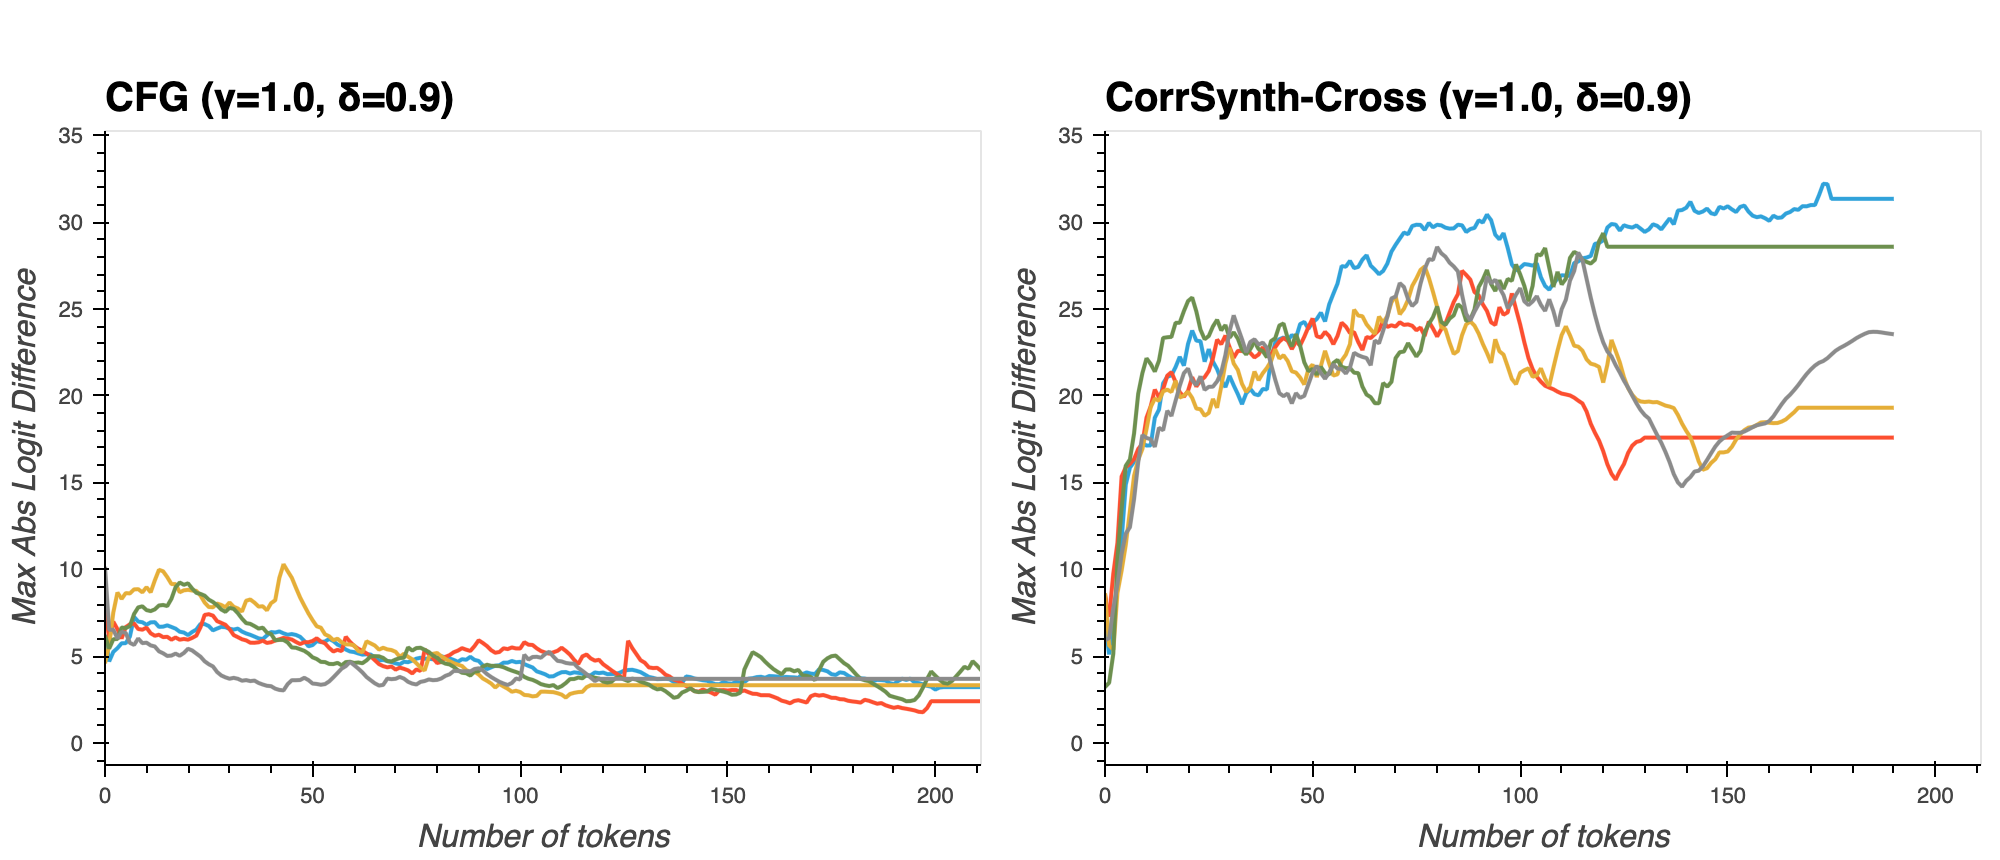
\includegraphics[width=0.5\textwidth]{figure/cfg_vs_corr.png}
\vspace{-0.8cm}
\caption{Generation progression from CFG and \corrsyn. We sample five generations using 3-shot prompts from \IMDb. The colored lines represent the absolute difference between logits of the current generation and contrast for each generation timestep (taken as an exponential moving average).}
\vspace{-1em}
\label{fig:cfg_vs_corrsynth}
\end{figure}


% \Category{}~\cite{blitzer-etal-2007-biographies} has Amazon product reviews and categories where the goal is to classify reviews into 23 categories, and hence in synthesis, we want to generate reviews for each of the categories. \Polarity~\cite{ni2019justifying} is Amazon product reviews dataset with positive and negative sentiment labels where the generation task involves asking the LLM to generate either a positive or a negative review for a a product. We do not provide any particular product to the LLM apart from those implicitly present in ICL examples. \Humor{} is a dataset about humorous and non-humorous questions about products. For generation, the label humorous or non-humorous is provided and the LLM is tasked to generate a corresponding question for any product on Amazon.



% \paragraph{Corpus.} In order to compare our results against \ours{} \citep{divekar2024synthesizrr} which uses retrieval-augmented generation for dataset synthesis, we use the five corpora mentioned in \autoref{tab:corpus} as the retrieval corpus. \RealNewsDom{} and \RealNewsInd{} are splits of news corpus \RealNews{} \citep{zellers2019grover}, which were filtered based by the country-headquarters of the news website \citep{divekar2024synthesizrr}. \Products{} contains metadata of products sold on e-commerce website Amazon \citep{ni-etal-2019-justifying}. Whereas \YelpCorpus{} corpus \cite{yelpcorpus} contains details of brick-and-mortar businesses listed on Yelp.com. \CMUMoviesCorpusShort{} corpus \cite{bamman-etal-2013-learning} contains 42k movie plot summaries. 

\paragraph{Teachers and students.} \ad{TODO fix this to be Mixtral. Cite.} As a teacher model, we use a frozen \Mixtral\ (8x7B) \citep{jiang2024mixtral} or \PhiMini\ (3.8B) \citep{abdin2024phi} for the data generation step. Following \citep{divekar2024synthesizrr}, we select examples randomly from the train set: 50 ICL examples per class for multi-class and 100 per class for binary. We think that this is a reasonable number of labeled examples since we are trading off the effort of labeling versus developing a potential zeroshot technique (which may not work well in practice). We use \DistilBERT{} student model (66M params \citet{Sanh2019DistilBERT}) as it is popular in prior work.

% Please add the following required packages to your document preamble:
% \usepackage{booktabs}
% \usepackage{multirow}
\begin{table*}[h]
\centering
\setlength{\tabcolsep}{3pt}
\begin{tabular}{
L{95pt}
% h
c % Teacher
c % C{16pt} % AG Accuracy
c % C{26pt} % IMDb Accuracy
c % C{16pt} % AG Mauve
c % C{26pt} % IMDb Mauve
c % C{16pt} % AG Self-BLEU-5
c % C{26pt} % IMDb Self-BLEU-5
c % C{16pt} % AG Entity Entropy
c % C{20pt} % IMDb Entity Entropy
}

\toprule
\multirow{2}{*}{\textbf{Method}}   
& \multirow{2}{*}{\textbf{Teacher}} %\multicolumn{1}{h}{\multirow{2}{*}{\textbf{Params}}}
% &  %\multicolumn{1}{C{26pt}}{\multirow{2}{*}{\textbf{Teacher}}}
& \multicolumn{2}{c}{\textbf{Accuracy}}
& \multicolumn{2}{c}{\textbf{MAUVE}}
& \multicolumn{2}{c}{\textbf{Self-BLEU-5}}
& \multicolumn{2}{c}{\textbf{Entity-Entropy}}
\\ 
\cmidrule(l){3-4}
\cmidrule(l){5-6}
\cmidrule(l){7-8}
\cmidrule(l){9-10} 
& \textbf{LM} % \multicolumn{1}{c}{\textbf{LM}}
& \textbf{{ } \AG} % AG Accuracy
& \textbf{\IMDb { }} % IMDb Accuracy
& \textbf{{ } \AG} % AG Mauve
& \textbf{\IMDb { }} % IMDb Mauve
& \textbf{{ } \AG} % AG Self-BLEU-5
& \textbf{\IMDb { }} % IMDb Self-BLEU-5
& \textbf{{ } \AG} % AG Entity Entropy
& \textbf{\IMDb { }} % IMDb Entity Entropy
\\ 
\midrule
\gold          
& -
& 91.4 & 91.4
& -	 & -	
& 17.1 & 27.9
& 6.6 & 7.5
\\ 
\midrule
%% 
%%
%%
\multicolumn{10}{c}{\underline{\textsc{Retrieval-based methods}}}  \\
\ReGen  
& \BERT
& 82.7 & $\otimes$
& 68.1 & $\otimes$
& 56.5 & $\otimes$
& \textbf{8.1 }& $\otimes$
\\ 
\SynthesizRR
& \LLaMa
& 84.6 & 84.8	
& \textbf{92.6} & 72.6	
& 34.2 & 62.9	
& 7.2 & 5.7
\\
\midrule 
%% 
%%
%%
\multicolumn{10}{c}{\underline{\textsc{Non-retrieval methods}}}  \\
\SunGen
& \GPTTwoXL
& $\otimes$ & 84.9	
& $\otimes$ & 68.7	
& $\otimes$ & \textbf{15.4}	
& $\otimes$ & 4.9
\\ 
\LetsSynth
& \ChatGPTShort
& $\otimes$ & \textbf{87.1}	
& $\otimes$ & 62.0	
& $\otimes$ & 62.2	
& $\otimes$ & 5.7
\\ 
\AttrPrompt
& \ChatGPTShort
& 79.8	& $\otimes$	
& 52.8	& $\otimes$	
& 39.8	& $\otimes$	
& 6.0	& $\otimes$
\vspace{1.5ex} 
\\ 
% \midrule 
% \multicolumn{10}{c}{\underline{\textsc{Ours}}}  \\
(Ours) \corrsynreallyshort-Intra
& \textsc{Phi-3 Mini}
& 84.8 & \textbf{87.1}
& 82.3 & \textbf{77.4}	
& 13.1 & 24.9	
& 7.4 & \textbf{6.5}
\\ 
(Ours) \corrsynreallyshort-Hybrid 
& \textsc{Phi-3 Mini}
& \textbf{85.1} & 86.8	
& 77.5 & 71.0	
& \textbf{12.1} & 19.2	
& 7.4 & 6.4
\\
\bottomrule
\end{tabular}
\caption{
Comparison of quality metrics and \DistilBERT\ student model fine-tuned on 6k rows from each approach. Mean accuracy across 5 training runs is considered. $\otimes$ indicates datasets were not released by authors.
}
\vspace{-1em}
\label{tab:baselines}
\end{table*}


\paragraph{Evaluation criteria} The task of evaluation of quality of text generation is quite challenging~\citep{llm-eval-survey}. Following prior works like \cite{divekar2024synthesizrr}, we evaluate synthetic generations based on several metrics. \textbf{Self-BLEU} \citep{bleu,zhu2018texygen} measures lexical diversity of a corpus of texts based on $n$-gram overlap between pairs of examples. \textbf{Entity entropy} measures the \textit{diversity} of entities in the generated texts using the distribution of each of 16 entity-types (inferred from a pre-trained named entity recognition model). Dataset which have high occurrence of few popular entities score lower on entropy. \textbf{MAUVE} \citep{liu-etal:divergence:neurips2021} measures closeness to human-written text using representations from a pre-trained \GPTTwoXL{} model. We also measure the \textbf{student accuracy} when trained on the synthetic data. We do not consider label preservation accuracy as it is susceptible to easy examples \cite{divekar2024synthesizrr}. In order to analyse the behavior of our strategy, we also study the label-wise cosine similarity of the generations, low dimensional embeddings of the generations using UMAP~\cite{mcinnes2020umap} and dataset cartography~\cite{swayamdipta-etal-2020-dataset}. %In addition, we also plot the visualizations of text representations of our generations against the \fewgen{} baseline as well (Section \ref{sec:analysis}).

\paragraph{Remark on diversity} In this work we are concerned about diversity at a dataset level and not an an instance level. To illustrate the difference between these two, consider the task of generating a long story. Here, it is important to ensure that the generated story has many of the features of a human written story (like complex storyline, many characters, non-repeating scenes etc.). But notice that ensuring such an instance level diversity does not guarantee diverse dataset of stories: multiple such stories obtained from an LLM could have a lot of overlap in content. For synthesis of good classification datasets, we require a more global notion of diversity which is at the dataset level. 

% In \S\ref{sec:student} we measure the effectiveness of synthetic data for student distillation. Besides the final performance of the student model, we also consider \textbf{label preservation accuracy}, the fraction of synthetic examples which are classified into prompted target class by an existing ``oracle'' model for the task. We construct the oracle by running a grid-search over \DeBERTaLarge{} hyperparams, splitting 80\% of the \gold{} train set for fine-tuning and 20\% for validation. %This metric is imperfect; it is possible to obtain very high label-preservation from a synthesis procedure generating easy-to-classify examples. These are of limited use for student generalization. Thus, we measure the training dynamics from the \textbf{Data Maps} generated by a \DistilBERT{} training run \citep{swayamdipta-etal-2020-dataset}. This identifies easy-to-learn, ambiguous and hard-to-learn synthetic examples.\gd{maybe revise or de-emphasize based on the final results}


\section{Results}
\label{sec:expts}

\subsection{Comparison to CFG}
We compare the effect of contrast as next-token generation proceeds in CFG and \corrsyn{}. To this end, we consider \IMDb{}, and sample continuations for five 3-shot prompts from both CFG and \corrsyn{} for the same Cross-label parameters: \mbox{$\{R=1, \gamma=1.0, \delta=0.9, \alpha=0\}$}. For each token, we store the maximum absolute difference of the current label logits vector and the contrast label logits vector (i.e. $\infty$-norm of logits difference of numerator and denominator in \eqref{eq:2corr_eq1} for \corrsyn{}, and similar terms in CFG). We plot this difference against the tokens generated. 

\autoref{fig:cfg_vs_corrsynth} shows the difference between CFG and \corrsyn{}: as token generation proceeds, the effect of contrast in CFG is muted. This happens since the same generated sequence for the current label is fed back into the contrast model and thus the effect of the contrastive prompt reduces over later token generations. Whereas in \corrsyn{}, the effect of the guidance or contrast persists. As a result, we believe \corrsyn{} is a better suited for longer generations where guidance is required for the entirety of generation. In terms of complexity, as discussed previously, we incur a much higher complexity of LLM model forward passes in CFG (detailed comparison in \aref{app:compute_complexity}). 


\subsection{Comparison to \fewgen}
\label{sec:corrsyn_results}
In this section, we present our experimental results against \fewgen. We use the following settings:

\insection[:]{\corrsyn{} Cross-label} Repeat factor $R=1$, Uniform contrastive guidance with \mbox{$\gamma=1.0 $} and $\delta=0.9\times\gamma$ and plausibility criterion $\alpha=10^{-3}$.

\insection[:]{\corrsyn{} Intra-label} Repeat factor $R=2$, Uniform contrastive guidance with \mbox{$\gamma=1.0 $} and $\delta=0.5\times\gamma$ and plausibility criterion $\alpha=10^{-3}$.

\insection[:]{\corrsyn{} Hybrid} Repeat factor $R=2$, set $\gamma=1.0$, Set $\gamma_{intra}=\gamma/2$, $\gamma_{cross}=\gamma/10$. Then uniform contrastive guidance in each of intra and cross terms. We set plausibility criterion \mbox{$\alpha=10^{-3}$}.
% \begin{itemize}
%     \item Cross-label \corrsyn\
%     \begin{itemize}
%         \item Repeat factor $R=1$
%         \item Uniform contrastive guidance with \mbox{$\gamma\in\{0.5,1.0,1.5\}$} and $\delta=0.9\times\gamma$
%         \item Plausibility criterion $\alpha=10^{-3}$
%     \end{itemize}
%     \item Hybrid \corrsyn\
%     \begin{itemize}
%         \item Set repeat factor $R=2$. 
%         \item Set $\gamma_{intra}=$, $\gamma_{cross}=$. Use uniform contrastive guidance within intra and cross contrasts: for intra, we set $\gamma_{m,n}=\frac{\gamma_{intra}}{R-1}$, and for cross $\gamma_{m,n}=\frac{\gamma_{cross}}{(K-1)R}$ where $K$ is the number of classes. 
%         \item Plausibility constraint $\alpha=10^{-3}$
%     \end{itemize}
% \end{itemize}


We observe in \autoref{tab:accuracy-diversity-icl} that 3-shot \corrsyn{} outperforms \fewgen{} on all evaluation metrics. Specifically, using Hybrid and Intra variants, we can achieve better student model accuracy (\DistilBERT) while increasing diversity (lower Self-BLEU, higher entity entropy) and better match with human-written text (better MAUVE). For MAUVE computation, we have used embeddings based on a GPT-2XL model. We have only shown the results for Intra and Hybrid variants since from our ablations they performed best. In \autoref{app:zeroshot}, we note the zero-shot results, which demonstrate comparable gains on all metrics. 





\begin{figure*}[!t] % Use figure* to span both columns
    \centering
    \begin{subfigure}[t]{\textwidth}
        \centering
        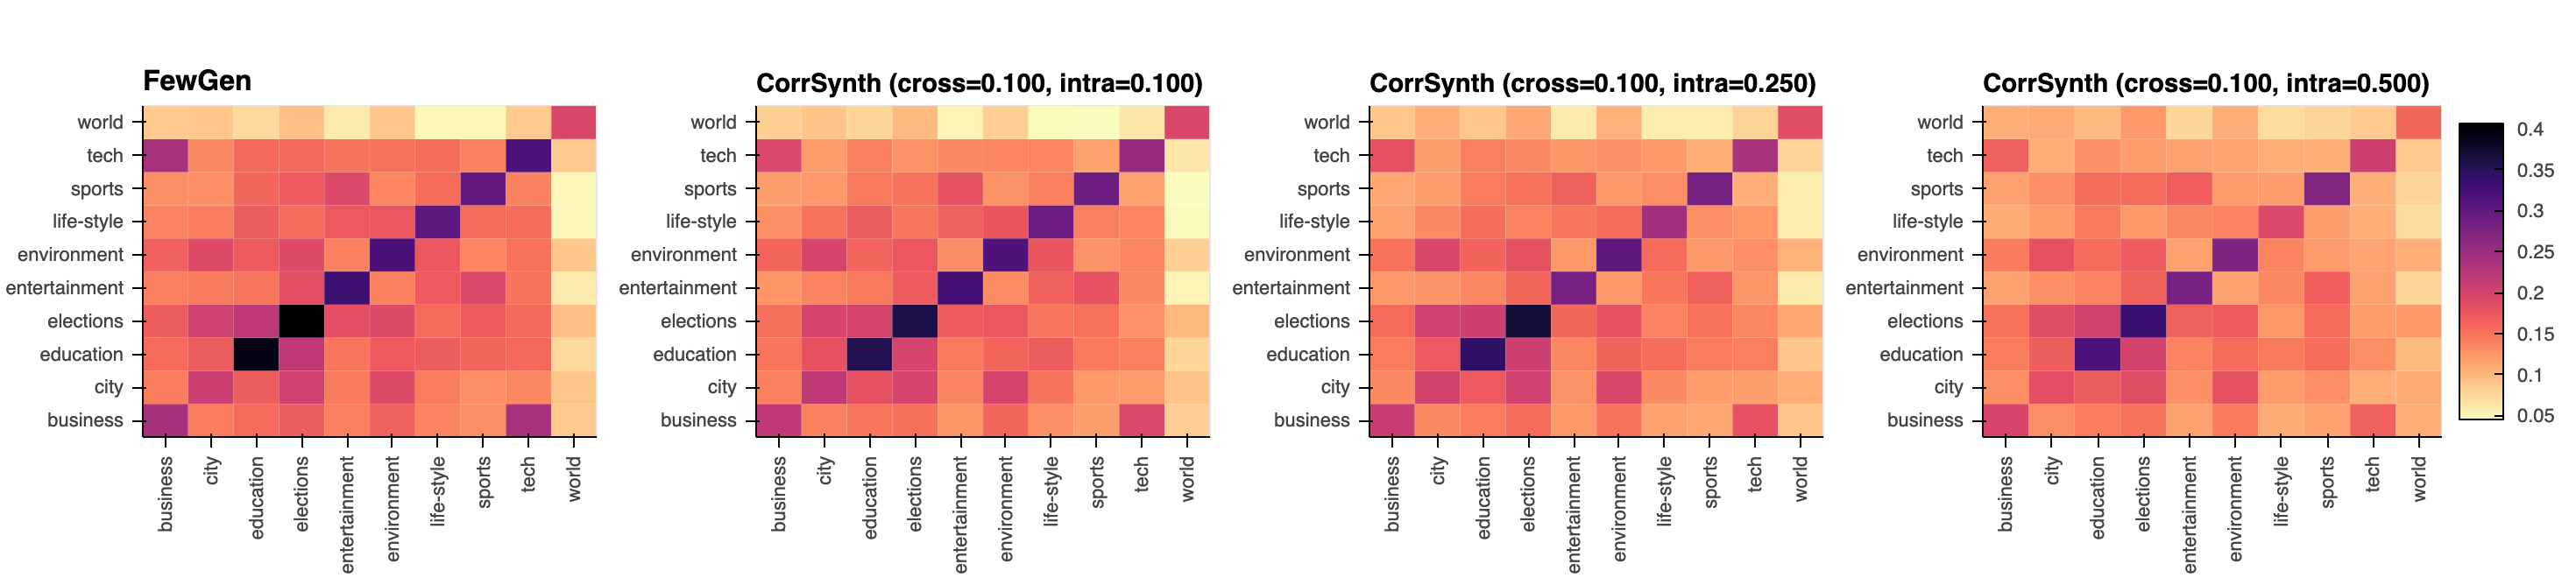
\includegraphics[width=\textwidth]{figure/cosine_intra_variation_v2.png}
        \caption{Impact of increasing Intra-label contrast (left to right) in Hybrid \corrsyn\ upon label-wise cosine similarities.}
        \label{fig:cosine_intra}
    \end{subfigure}
    \vskip\baselineskip
    \vspace{-0.7cm}
    \begin{subfigure}[t]{\textwidth}
        \centering
        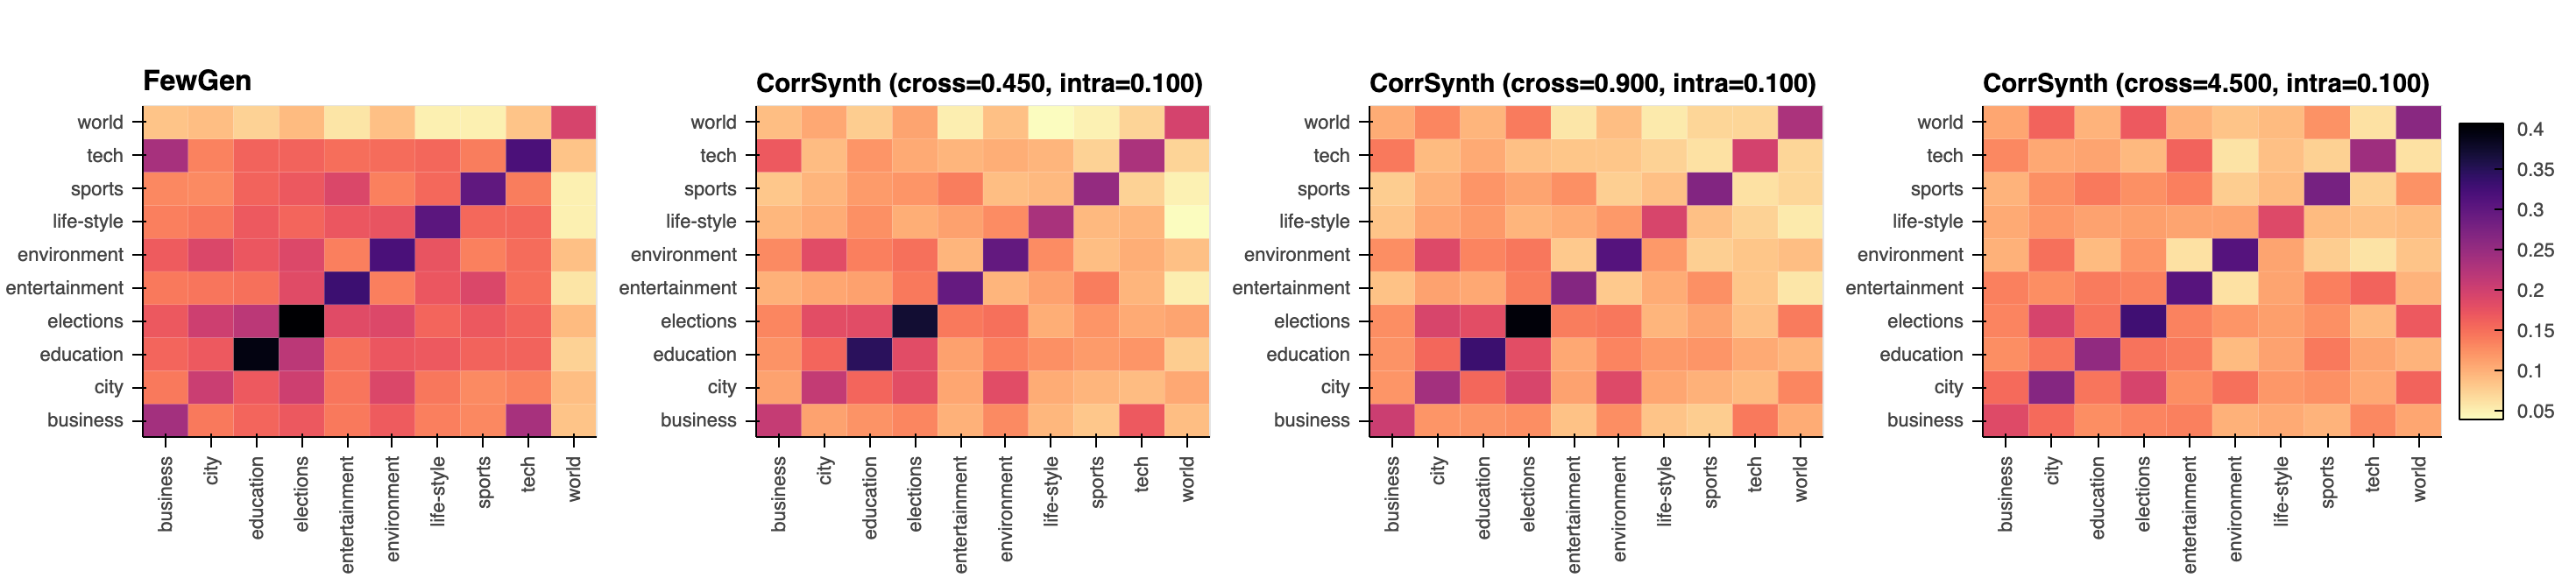
\includegraphics[width=\textwidth]{figure/cosine_cross_variation_v2.png}
        \caption{Impact of increasing Cross-label contrast (left to right) in Hybrid \corrsyn\ upon label-wise cosine similarities.}
        \label{fig:cosine_cross}
    \end{subfigure}
    \caption{Heatmaps for label-wise cosine similarities on \ToIHeadlines\ (with Phi-3-mini) as we increase Intra-label contrast vs increasing cross-label contrast. Note that ``Cross'' and ``Intra'' in figure titles correspond to $\gamma_{cross}$ and $\gamma_{intra}$ respectively. \fewgen\ heatmaps are provided for reference.}
    \vspace{-1em}
    \label{fig:cosine}
\end{figure*}





\subsection{Comparison to prior works} 

In \autoref{tab:baselines} we compare \corrsyn{} to current dataset generation methods as baselines. Baseline numbers are quoted from \citet{divekar2024synthesizrr}, where all results are reported on 6k rows using \DistilBERT\ student (same as our setup). The following SOTA generation methods have been compared: 
(1) \textbf{\ReGen{}} \cite{yu-etal-2023-regen}: uses dual BERT models - one for retrieval and one as a classifier - to perform multi-round filtering and eliminate noisy data based on model consistency; 
(2) \textbf{\SynthesizRR{}} \cite{divekar2024synthesizrr}: develops a hybrid retrieval-augmentation based approach to rewrite contexts, greatly enhancing the diversity of generated text;
(3) \textbf{\SunGen{}} \cite{gao2023selfguided}: employs \ZeroGen{} \cite{ye2022zerogen} to create a substantial synthetic dataset (200k rows) and then uses a bi-level optimization algorithm to assign instance-weights to each synthetic example; 
(4) \textbf{\LetsSynth{}} \cite{wang-etal-2023-lets}: builds a distinct ``seed dataset'' to train a student model, leverages an LLM to identify errors, and synthesizes supplementary data. This cycle of data augmentation is repeated.
(5) \textbf{\AttrPrompt{}} \cite{yu2023large}: enhances dataset diversity and unbiasedness by prompting a potent LLM like \ChatGPT{} with attributes identified through human-in-the-loop task analysis.

We divide our comparison into non-retrieval and retrieval based synthesis, as the latter naturally demonstrates higher diversity \citep{divekar2024synthesizrr}. We observe that \corrsyn{} achieves strong performance on all metrics, despite using a small teacher LLM (\PhiMini with 3.8B parameters) compared to prior approaches. 




\begin{figure*}[!t]
\centering
    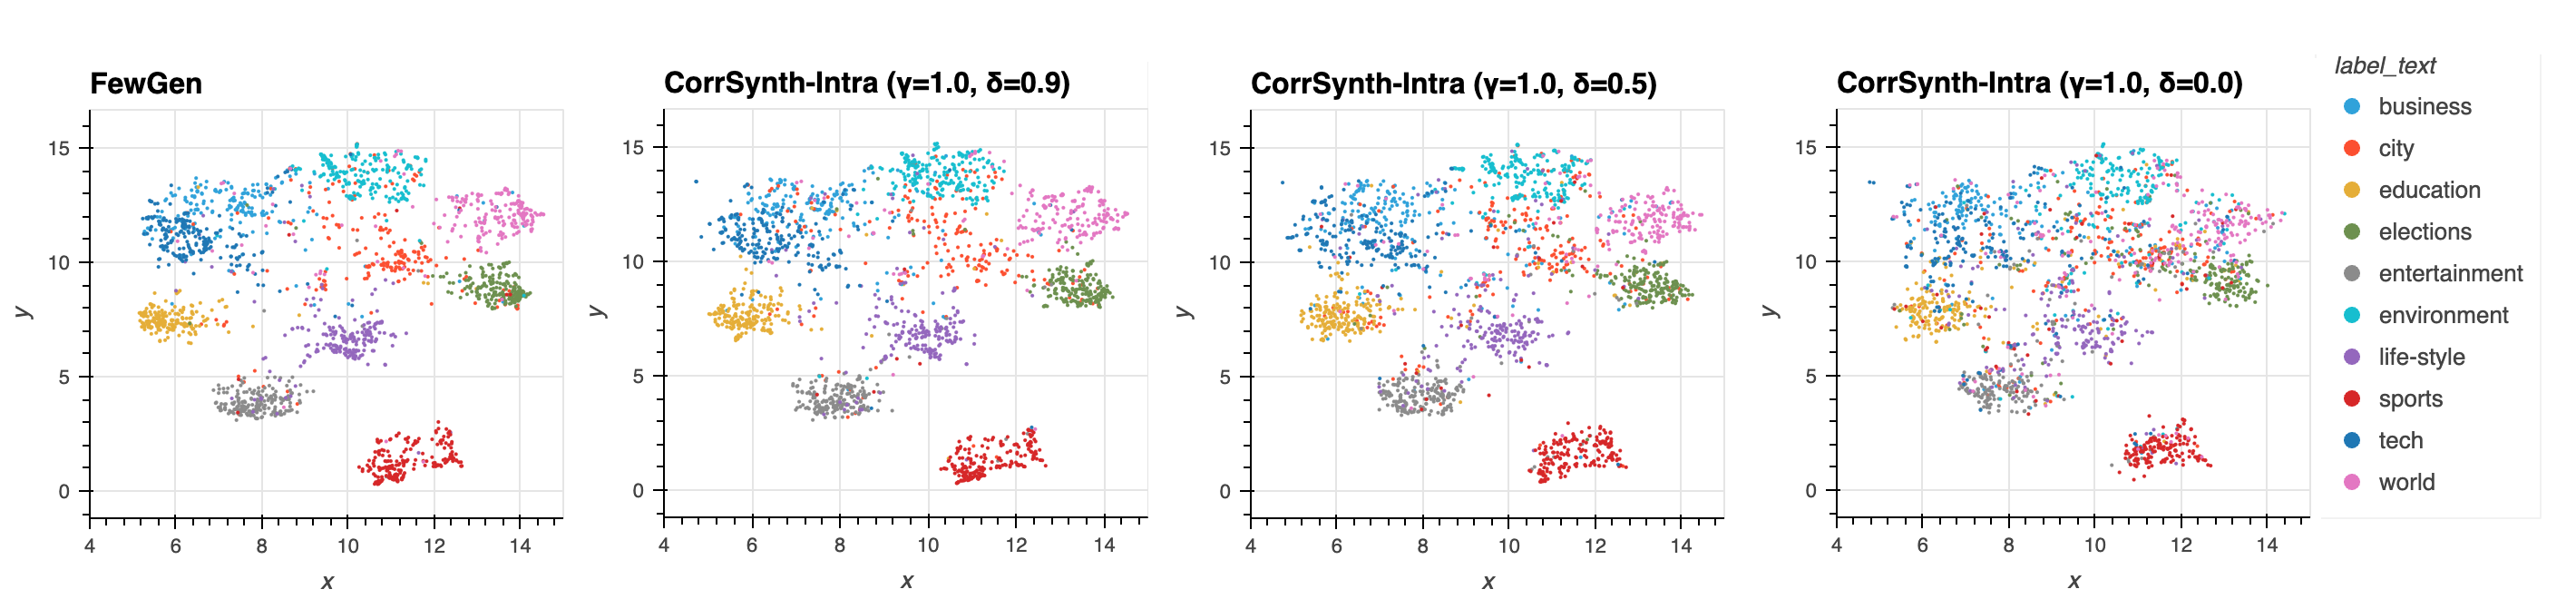
\includegraphics[width=\textwidth]{figure/umaps_v3.png}
    \vspace{-0.8cm}
    \caption{Visualising two-dimensional text representations of generations (on \ToIHeadlines\ with \PhiMini) using \corrsyn-Intra. We gradually increase guidance delta, $\delta$ in $(0.0, 0.5, 0.9)$. \fewgen\ plot is provided as a reference to the unmodified clusters (it is equivalent to $\delta=1$ i.e. no contrast).}
    \vspace{-1em}
    \label{fig:intra_label_umaps}
\end{figure*}





%Additional intrinsic analysis in \autoref{ta:bmauve} shows that the generations from \corrsyn{} more closely match human-written text in terms of Mauve (which generates embeddings based on a GPT-2XL model). Thus we are able to achieve much more realistic text through our approach. 
% \ad{Merge MAUVE with main results table}



% % Please add the following required packages to your document preamble:
% % \usepackage{booktabs}
% % \usepackage{multirow}
% \begin{table*}[h]
% \centering
% \begin{tabular}{
% L{18pt}
% C{18pt}
% C{18pt}
% C{18pt}
% C{18pt}
% C{18pt}
% C{18pt}
% C{18pt}
% C{18pt}
% }
% \toprule
% \multicolumn{1}{l}{\multirow{2}{*}{\textbf{Method}}} & \multicolumn{1}{c}{\multirow{2}{*}{\textbf{Source}}} & \multicolumn{1}{c|}{\multirow{2}{*}{\textbf{Teacher LM}}} & \multicolumn{3}{c|}{\textbf{Sentiment}}                    & \multicolumn{3}{c}{\textbf{Topic}}                            \\ 

% \cmidrule(l){2-7} 

% \multicolumn{1}{l|}{}                     & \textbf{\Pol} & \textbf{\Yelp} & \multicolumn{1}{c|}{\textbf{\IMDb}} & \textbf{\AG} & \textbf{\ToI} & \textbf{\Cat} \\ \midrule
% \multicolumn{1}{l|}{\gold}                 & 0     & 0             & \multicolumn{1}{c|}{0}             & 0    & 0          & 0                 \\ \midrule
% \multicolumn{7}{c}{\underline{\textsc{Zero-shot}}}                                                                                                                                                         \\
% \multicolumn{1}{l|}{\AttrPrompt}           & 0     & 0             & \multicolumn{1}{c|}{0}             & 0    & 0          & 0                 \\
% \multicolumn{1}{l|}{\fewgen}               & 0     & 0             & \multicolumn{1}{c|}{0}             & 0    & 0          & 0                 \\
% \multicolumn{1}{l|}{\ours}          & 0     & 0             & \multicolumn{1}{c|}{0}             & 0    & 0          & 0                 \\
% \multicolumn{1}{l|}{\corrsyn}            & 0     & 0             & \multicolumn{1}{c|}{0}             & 0    & 0          & 0                 \\ \midrule
% \multicolumn{7}{c}{\underline{\textsc{Few-shot (Human seed)}}}                                                                                                                                             \\
% \multicolumn{1}{l|}{\Human\ ICL + \fewgen}    & 0     & 0             & \multicolumn{1}{c|}{0}             & 0    & 0          & 0                 \\
% \multicolumn{1}{l|}{\Human\ ICL + \oursshort}      & 0     & 0             & \multicolumn{1}{c|}{0}             & 0    & 0          & 0                 \\
% \multicolumn{1}{l|}{\Human\ ICL + \corrsyn}             & 0     & 0             & \multicolumn{1}{c|}{0}             & 0    & 0          & 0                 \\ \midrule
% \multicolumn{7}{c}{\underline{\textsc{Few-shot (Generated seed)}}}                                                                                                                                         \\
% \multicolumn{1}{l|}{\fewgen\ ICL + \fewgen}            & 0     & 0             & \multicolumn{1}{c|}{0}             & 0    & 0          & 0                 \\
% \multicolumn{1}{l|}{\fewgen\ ICL + \oursshort}     & 0     & 0             & \multicolumn{1}{c|}{0}             & 0    & 0          & 0                 \\
% \multicolumn{1}{l|}{\corrsyn\ ICL + \fewgen}            & 0     & 0             & \multicolumn{1}{c|}{0}             & 0    & 0          & 0                 \\
% \multicolumn{1}{l|}{\corrsyn\ ICL + \oursshort}  & 0     & 0             & \multicolumn{1}{c|}{0}             & 0    & 0          & 0                 \\ \bottomrule
% \end{tabular}
% \caption{Performance comparison of student model (DistilBERT) fine-tuned on generated datasets on each method. We report mean accuracy numbers across 5 runs (The standard deviation across the runs was $<0.5$, hence, we do not report it.)}
% \end{table*}






% % % Please add the following required packages to your document preamble:
% % \usepackage{booktabs}
% % \usepackage{multirow}
% \begin{table}[]
% \small
% \centering
% \begin{tabular}{
% L{38pt}
% C{16pt} 
% C{16pt}
% C{20pt} |
% C{16pt}
% C{16pt}
% C{16pt}
% }
% \toprule
% \multirow{2}{*}{\textbf{Method}} 
% & \multicolumn{3}{c|}{\textbf{Sentiment}}      
% & \multicolumn{3}{c}{\textbf{Topic}}        
% \\ 
% \cmidrule(l){2-7} 
% & \textbf{\Pol} 
% & \textbf{\Yelp} 
% & \textbf{\IMDb} 
% & \textbf{\AG} 
% & \textbf{\ToI} 
% & \textbf{\Cat} 
% \\ \midrule
% % \gold             
% % & 0            & 0             & 0             & 0           & 0            & 0            \\
% \AttrPromptShort             
% & -            & 55.9          & -          & 52.8      & -            & -            \\
% \fewgen             
% & 65.2         & 80.4          & 60.8       & 78.4      & 67.8         & 64.1         \\
% \oursshort            
% & -            & 76.6          & 60.3       & 94.0      & 71.7         & 65.0         \\ 
% \corrsynshort             
% & 71.8         & 85.5          & 66.9       & 86.2      & 74.9         & -            \\ 
% \bottomrule
% \end{tabular}
% \caption{Mauve results (3-shot Human-annotated ICL set). Synthesis results are generated from \textsc{Mistral-7B-Instruct} teacher LM.}
% \label{tab:mauve}
% \end{table}


% \begin{table}[h]
% \centering
% \sisetup{round-mode=places, round-precision=1} % Set the rounding precision
% \setlength{\tabcolsep}{1.9pt}
% \footnotesize{
% \scalebox{0.9}{
% \begin{tabular}{
% C{1.65cm}  % Method
% C{1.45cm}  % Teacher LM
% C{2.7cm}  % Retriever
% c % S[table-format=3.2]  % Yelp Self-BLEU
% c % S[table-format=3.2]  % AG News Self-BLEU
% c % S[table-format=3.2]  % IMDb Self-BLEU
% c % S[table-format=3.2]  % SST-2 Self-BLEU
% % c 
% |c % S[table-format=3.2]  % Yelp Entity Entropy
% c % S[table-format=3.2]  % AG News Entity Entropy
% c % S[table-format=3.2]  % IMDb Entity Entropy
% c  % S[table-format=3.2]  % SST-2 Entity Entropy
% % c 
% |c % S[table-format=3.2]  % Yelp Mauve
% c % S[table-format=3.2]  % AG News Mauve
% c % S[table-format=3.2]  % IMDb Mauve
% c % S[table-format=3.2]  % SST-2 Mauve
% }
% \toprule
% % \multirow{3}{*}{\textbf{Method}}
% % & \multirow{3}{*}{ \textbf{Student LM} }
% % & \multicolumn{1}{c}{\underline{\RNInd}} 
% % & \multicolumn{2}{c}{\underline{\RNDom}} 
% % & \multicolumn{3}{c}{\underline{\Products}} 
% % & \multirow{3}{*}{\textbf{Avg}}
% % \\
% % [0.5ex]
% \textbf{Method}
% & \textbf{Teacher}
% & \multirow{2}{*}{\textbf{Params}}
% & \multicolumn{4}{c}{\underline{Self-BLEU-5 \lowerbetter}} 
% % &
% & \multicolumn{4}{c}{\underline{Entity Entropy \higherbetter}} 
% % &
% & \multicolumn{4}{c}{\underline{Mauve \higherbetter}} 
% \\
% [0.7ex]
% \textit{(Dataset)}
% & \textbf{LM}
% & 
% & \AG % Self-BLEU
% & \ToI % Self-BLEU
% & \Pol % Self-BLEU
% & \Hum % Self-BLEU
% % & 
% & \AG % Self-BLEU
% & \ToI % Self-BLEU
% & \Pol % Self-BLEU
% & \Hum % Self-BLEU
% % & 
% & \AG % Self-BLEU
% & \ToI % Self-BLEU
% & \Pol % Self-BLEU
% & \Hum % Self-BLEU
% \\ 
% \midrule
%  \gold &  - & - 
%  & 11.3  &  5.9  & 14.4   &  15.0 
%  & 5.8   & 5.3   &  6.0  &  3.9 
%  &  -  &  -  &  -  & -   
%  \vspace{0.75ex} \\ 

%  \toprule
% \multicolumn{15}{c}{\underline{\textsc{3- shot}}} \vspace{1ex} \\
% \fewgen &  \LLaMa & \_ &  23.6  &  18.5  &  50.5  &  36.8  &  5.5  &  5.0  &  3.8  &  3.2  &  96.5  &  97.7  &  81.9  &  94.2 \\
%  \corrsyn &  \LLaMa & $\gamma=0.5, \delta=0.45$ 
%  &  \best{6.4}  &  \best{6.0}  &  \best{7.4}  &  \best{10.1}  
%  &  6.0  &  \best{5.3}  &  5.6  &  \best{4.0} 
%  &  96.2  &  98.2  &  \best{90.6}  &  \best{99.7}  \\
%  \corrsyn &  \LLaMa & $\gamma=0.5, \delta=0.5$ 
%  &  6.7  &  6.4  & 7.9  &  10.7  
%  &  \best{6.1}  &  5.2  &  \best{5.7}  &  3.9  
%  &  95.8  &  98.0  &  88.1  &  \best{99.7}  \\
%  \corrsyn &  \LLaMa & $\gamma=1.0, \delta=0.9$ 
% & 20.8  &  14.4  & 43.9   &  30.1  
%  & 5.5   & 4.9   &  3.8  &  3.0
%  & \best{96.7}   &  \best{98.8}  &  82.1  & 96.1   \\
%  \corrsyn &  \LLaMa & $\gamma=1.0, \delta=1.0$ 
%  & 22.4  &  17.9  & 48.6   &  32.7  
%  & 5.6   & 5.0   &  4.1  &  2.9
%  &  96.4  &  98.7  &  80.1  & 94.6   \\
%   \corrsyn &  \LLaMa & $\gamma=1.5, \delta=1.35$ 
%  & 37.4  &  30.9  & 67.8   &  54.4  
%  & 5.1   & 4.6   &  3.1  &  2.8
%  &  94.6  &  98.0  &  72.2  & 91.9   \\
%   \corrsyn &  \LLaMa & $\gamma=1.5, \delta=1.5$ 
%  & 40.2  &  35.1  & 70.3   &  59.7  
%  & 5.5   & 4.4   &  2.9  &  2.5
%  &  91.4  &  97.7  &  70.4  & 88.6   \\
% [0.75ex]
% \bottomrule
% \end{tabular}
% }
% }
% \caption{
% Intrinsic evaluations of synthetic datasets generated by \fewgen\ and \corrsyn. We also compare against the gold dataset. We subsample all to 2k examples before computing metrics. Within each dataset, we \textbf{bold} the best result.
% }
% \vspace{-3ex}
% \label{tab:baselines-intrinsic}
% \end{table}



% \section{Ablations}
% \label{sec:ablations}
% In this section we provide our ablation results. We measure the variation of \textbf{Self-BLEU}, \textbf{Entity entropy}, \textbf{MAUVE} and \textbf{student accuracy} as we vary each parameter by keeping others fixed. In particular we vary i) guidance $\gamma\in \{0.1,0.5,1.0,1.5,3,10\}$\sk{what is the final grid for gamma}, ii) $\delta\in\{0,1.0,0.5\gamma,0.95\gamma,\gamma,1.05\gamma,\}$\sk{what is the final grid for delta?}, iii) repeat factor $R\in\{1,3\}$, iv) contrast type in cross-label v/s hybrid\sk{rewrite hybrid, by removing ration}



% % Please add the following required packages to your document preamble:
% % \usepackage{booktabs}
% \begin{table}[]\small
% \centering
% \begin{tabular}{@{}lccccc@{}}
% \toprule
% \textbf{Method} & \textbf{Params} & \AGNews    & \ToI  & \Polarity & \Humor \\ \midrule
% \gold            & \_              & 88.78          & 75.08         & 89.68             & 91.56          \\ \midrule
% \fewgen          & \_              & 84.08          & 69.96         & 86.34             & 86.74          \\
% \corrsyn            & $\gamma=0.5, \delta=0.45$              & 84.47          & \textbf{72.2} & 88.26             & \textbf{88.00} \\
% \corrsyn            & $\gamma=0.5, \delta=0.5$              & 84.43          & 70.68         & \textbf{88.60}    & 87.05          \\
% \corrsyn            & $\gamma=1.0, \delta=0.9$              & 83.76          & 69.33         & 86.39             & 87.62          \\
% \corrsyn            & $\gamma=1.0, \delta=1.0$              & 84.16          & 68.72         & 85.75             & 86.81          \\
% \corrsyn            & $\gamma=1.5, \delta=1.35$              & \textbf{84.59} & 70.06         & 84.59             & 86.16          \\
% \corrsyn            & $\gamma=1.5, \delta=1.5$              & 84.17          & 68.31         & 85.71             & 85.13          \\ \bottomrule
% \end{tabular}
% \caption{Performance comparison of student model (DistilBERT) fine-tuned on generated datasets on each method. We report mean accuracy numbers across 5 runs (The standard deviation across the runs was $<0.5$, hence, we do not report it.)}
% \end{table}



% \begin{table}[!h]
% \centering
% \sisetup{round-mode=places, round-precision=1} % Set the rounding precision
% \setlength{\tabcolsep}{2pt}
% \footnotesize{
% \begin{tabular}{
% l
% c
% h % L{2.4cm}  % Student
% S[table-format=3.2]  % ToI
% S[table-format=3.2] S[table-format=3.2] % Realnews 
% S[table-format=3.2] S[table-format=3.2] S[table-format=3.2] % Products
% l  % Average
% }
% \toprule
% % \multirow{3}{*}{\textbf{Method}}
% % & \multirow{3}{*}{ \textbf{Student LM} }
% % & \multicolumn{1}{c}{\underline{\RNInd}} 
% % & \multicolumn{2}{c}{\underline{\RNDom}} 
% % & \multicolumn{3}{c}{\underline{\Products}} 
% % & \multirow{3}{*}{\textbf{Avg}}
% % \\
% % [0.5ex]
% \textbf{Method}
% & \multirow{2}{*}{\textbf{Teacher LM}}
% &  
% & \AG{}  
% & \Humor{} 
% & \Intent{} 
% & \multirow{2}{*}{\textbf{Avg}}
% \\
% \textit{(Dataset size)}
% & 
% & 
% & \text{($2$K)}
% & \text{($2$K)}
% & \text{($2$K)}
% &
% \\ 
% % &                   &         &         &         &         &         &  \\ 
% % \cmidrule{1-2}                        \cmidrule{3-5} \cmidrule{7-9}
% % [-0.5ex]
% \midrule
% \gold &
% % & \TinyBERT{}       &     77.83 &         87.9 &       81.23 &         70.41 &      89.22 &         87.09 & 82.28 \\
% % & \DistilBERT{}     &     82.16 &        90.45 &       88.92 &         78.44 &      91.69 &         90.78 & 87.07 \\
% & \DeBERTa{}         &   &   &   & 
% % \vspace{1ex}
% \\

% %  ____                 ___  _          _
% % |_  / ___  _ _  ___  / __|| |_   ___ | |_
% %  / / / -_)| '_|/ _ \ \__ \| ' \ / _ \|  _|
% % /___|\___||_|  \___/ |___/|_||_|\___/ \__|

% % \midrule
% % \vspace{2ex}
% \toprule
% % \multicolumn{6}{c}{\underline{\textsc{Zero shot}}} \vspace{1ex} \\
% % \fewgen & \LLaMa
% % & \TinyBERT{}        &  71.96 &  62.69 &  57.85 &    48.0 &  83.15 &  74.55 & 66.37 \\
% % & \DistilBERT{}      &  59.45 &  66.56 &  58.77 &  57.79 &  67.74 &  80.37 & 65.11 \\
% % & \DeBERTa{} &  49.82 &  64.45 &  70.46 &  57.25 &  70.31 &  87.69 & 66.66 \\
% % & \DeBERTa{} &   &   &   &
% % \\
% % [1ex] 

% % \midrule

% \corrsyn & \LLaMa 
% % & \TinyBERT{}        &  68.56 &  84.06 &  58.15 &   61.5 &  78.15 &  79.45 & 71.64 \\
% % & \DistilBERT{}      &  72.86 &  85.54 &   60.0 &  70.97 &  79.91 &  79.71 & 75.11 (74.83) \\
% % & \DeBERTa{} &  73.95 &  85.55 &  70.15 &  70.12 &  85.71 &  88.02 & 78.92 
% & \DeBERTa{} &  &   &   &
% \vspace{1.5ex}
% \\

% \toprule
% \multicolumn{6}{c}{\underline{\textsc{Few shot}}} \vspace{1ex} \\
% \fewgen & \LLaMa
% % & \TinyBERT{}        &  71.96 &  62.69 &  57.85 &    48.0 &  83.15 &  74.55 & 66.37 \\
% % & \DistilBERT{}      &  59.45 &  66.56 &  58.77 &  57.79 &  67.74 &  80.37 & 65.11 \\
% % & \DeBERTa{} &  49.82 &  64.45 &  70.46 &  57.25 &  70.31 &  87.69 & 66.66 \\
% & \DeBERTa{} &   &   &   &
% \\
% % [1ex] 

% % \midrule

% \corrsyn & \LLaMa 
% % & \TinyBERT{}        &  68.56 &  84.06 &  58.15 &   61.5 &  78.15 &  79.45 & 71.64 \\
% % & \DistilBERT{}      &  72.86 &  85.54 &   60.0 &  70.97 &  79.91 &  79.71 & 75.11 (74.83) \\
% % & \DeBERTa{} &  73.95 &  85.55 &  70.15 &  70.12 &  85.71 &  88.02 & 78.92 
% & \DeBERTa{} &  &   &   &
% \vspace{1.5ex}
% \\




                                
% \bottomrule
% \end{tabular}
% }
% \caption{Accuracy}
% \label{tab:student-deb}
% \end{table}



% \begin{table}[!h]
% \centering
% \sisetup{round-mode=places, round-precision=1} % Set the rounding precision
% \setlength{\tabcolsep}{2pt}
% \footnotesize{
% \begin{tabular}{
% l
% c
% h % L{2.4cm}  % Student
% S[table-format=3.2]  % ToI
% S[table-format=3.2] S[table-format=3.2] % Realnews 
% S[table-format=3.2] S[table-format=3.2] S[table-format=3.2] % Products
% l  % Average
% }
% \toprule
% % \multirow{3}{*}{\textbf{Method}}
% % & \multirow{3}{*}{ \textbf{Student LM} }
% % & \multicolumn{1}{c}{\underline{\RNInd}} 
% % & \multicolumn{2}{c}{\underline{\RNDom}} 
% % & \multicolumn{3}{c}{\underline{\Products}} 
% % & \multirow{3}{*}{\textbf{Avg}}
% % \\
% % [0.5ex]
% \textbf{Method}
% & \multirow{2}{*}{\textbf{Teacher LM}}
% &  
% & \AG{}  
% & \Humor{} 
% & \Intent{} 
% & \multirow{2}{*}{\textbf{Avg}}
% \\
% \textit{(Dataset size)}
% & 
% & 
% & \text{($2$K)}
% & \text{($2$K)}
% & \text{($2$K)}
% &
% \\ 
% % &                   &         &         &         &         &         &  \\ 
% % \cmidrule{1-2}                        \cmidrule{3-5} \cmidrule{7-9}
% % [-0.5ex]
% \midrule
% \gold &
% % & \TinyBERT{}       &     77.83 &         87.9 &       81.23 &         70.41 &      89.22 &         87.09 & 82.28 \\
% % & \DistilBERT{}     &     82.16 &        90.45 &       88.92 &         78.44 &      91.69 &         90.78 & 87.07 \\
% & \DeBERTa{}         &   &   &   & 
% % \vspace{1ex}
% \\

%  ____                 ___  _          _
% |_  / ___  _ _  ___  / __|| |_   ___ | |_
%  / / / -_)| '_|/ _ \ \__ \| ' \ / _ \|  _|
% /___|\___||_|  \___/ |___/|_||_|\___/ \__|

% \midrule
% \vspace{2ex}
% \toprule
% \multicolumn{6}{c}{\underline{\textsc{Zero shot}}} \vspace{1ex} \\
% \fewgen & \LLaMa
% % & \TinyBERT{}        &  71.96 &  62.69 &  57.85 &    48.0 &  83.15 &  74.55 & 66.37 \\
% % & \DistilBERT{}      &  59.45 &  66.56 &  58.77 &  57.79 &  67.74 &  80.37 & 65.11 \\
% % & \DeBERTa{} &  49.82 &  64.45 &  70.46 &  57.25 &  70.31 &  87.69 & 66.66 \\
% & \DeBERTa{} &   &   &   &
% \\
% % [1ex] 

% % \midrule

% \corrsyn & \LLaMa 
% % & \TinyBERT{}        &  68.56 &  84.06 &  58.15 &   61.5 &  78.15 &  79.45 & 71.64 \\
% % & \DistilBERT{}      &  72.86 &  85.54 &   60.0 &  70.97 &  79.91 &  79.71 & 75.11 (74.83) \\
% % & \DeBERTa{} &  73.95 &  85.55 &  70.15 &  70.12 &  85.71 &  88.02 & 78.92 
% & \DeBERTa{} &  &   &   &
% \vspace{1.5ex}
% \\

% \toprule
% \multicolumn{6}{c}{\underline{\textsc{Few shot}}} \vspace{1ex} \\
% \fewgen & \LLaMa
% % & \TinyBERT{}        &  71.96 &  62.69 &  57.85 &    48.0 &  83.15 &  74.55 & 66.37 \\
% % & \DistilBERT{}      &  59.45 &  66.56 &  58.77 &  57.79 &  67.74 &  80.37 & 65.11 \\
% % & \DeBERTa{} &  49.82 &  64.45 &  70.46 &  57.25 &  70.31 &  87.69 & 66.66 \\
% & \DeBERTa{} &   &   &   &
% \\
% % [1ex] 

% % \midrule

% \corrsyn & \LLaMa 
% % & \TinyBERT{}        &  68.56 &  84.06 &  58.15 &   61.5 &  78.15 &  79.45 & 71.64 \\
% % & \DistilBERT{}      &  72.86 &  85.54 &   60.0 &  70.97 &  79.91 &  79.71 & 75.11 (74.83) \\
% % & \DeBERTa{} &  73.95 &  85.55 &  70.15 &  70.12 &  85.71 &  88.02 & 78.92 
% & \DeBERTa{} &  &   &   &
% \vspace{1.5ex}
% \\




                                
% \bottomrule
% \end{tabular}
% }
% \caption{BLEU}
% \label{tab:student-deb}
% \end{table}



% \begin{table}[!h]
% \centering
% \sisetup{round-mode=places, round-precision=1} % Set the rounding precision
% \setlength{\tabcolsep}{2pt}
% \footnotesize{
% \begin{tabular}{
% l
% c
% h % L{2.4cm}  % Student
% S[table-format=3.2]  % ToI
% S[table-format=3.2] S[table-format=3.2] % Realnews 
% S[table-format=3.2] S[table-format=3.2] S[table-format=3.2] % Products
% l  % Average
% }
% \toprule
% % \multirow{3}{*}{\textbf{Method}}
% % & \multirow{3}{*}{ \textbf{Student LM} }
% % & \multicolumn{1}{c}{\underline{\RNInd}} 
% % & \multicolumn{2}{c}{\underline{\RNDom}} 
% % & \multicolumn{3}{c}{\underline{\Products}} 
% % & \multirow{3}{*}{\textbf{Avg}}
% % \\
% % [0.5ex]
% \textbf{Method}
% & \multirow{2}{*}{\textbf{Teacher LM}}
% &  
% & \AG{}  
% & \Humor{} 
% & \Intent{} 
% & \multirow{2}{*}{\textbf{Avg}}
% \\
% \textit{(Dataset size)}
% & 
% & 
% & \text{($2$K)}
% & \text{($2$K)}
% & \text{($2$K)}
% &
% \\ 
% % &                   &         &         &         &         &         &  \\ 
% % \cmidrule{1-2}                        \cmidrule{3-5} \cmidrule{7-9}
% % [-0.5ex]
% \midrule
% \gold &
% % & \TinyBERT{}       &     77.83 &         87.9 &       81.23 &         70.41 &      89.22 &         87.09 & 82.28 \\
% % & \DistilBERT{}     &     82.16 &        90.45 &       88.92 &         78.44 &      91.69 &         90.78 & 87.07 \\
% & \DeBERTa{}         &   &   &   & 
% % \vspace{1ex}
% \\

% %  ____                 ___  _          _
% % |_  / ___  _ _  ___  / __|| |_   ___ | |_
% %  / / / -_)| '_|/ _ \ \__ \| ' \ / _ \|  _|
% % /___|\___||_|  \___/ |___/|_||_|\___/ \__|

% % \midrule
% % \vspace{2ex}
% \toprule
% \multicolumn{6}{c}{\underline{\textsc{Zero shot}}} \vspace{1ex} \\
% \fewgen & \LLaMa
% % & \TinyBERT{}        &  71.96 &  62.69 &  57.85 &    48.0 &  83.15 &  74.55 & 66.37 \\
% % & \DistilBERT{}      &  59.45 &  66.56 &  58.77 &  57.79 &  67.74 &  80.37 & 65.11 \\
% % & \DeBERTa{} &  49.82 &  64.45 &  70.46 &  57.25 &  70.31 &  87.69 & 66.66 \\
% & \DeBERTa{} &   &   &   &
% \\
% % [1ex] 

% % \midrule

% \corrsyn & \LLaMa 
% % & \TinyBERT{}        &  68.56 &  84.06 &  58.15 &   61.5 &  78.15 &  79.45 & 71.64 \\
% % & \DistilBERT{}      &  72.86 &  85.54 &   60.0 &  70.97 &  79.91 &  79.71 & 75.11 (74.83) \\
% % & \DeBERTa{} &  73.95 &  85.55 &  70.15 &  70.12 &  85.71 &  88.02 & 78.92 
% & \DeBERTa{} &  &   &   &
% \vspace{1.5ex}
% \\

% \toprule
% \multicolumn{6}{c}{\underline{\textsc{Few shot}}} \vspace{1ex} \\
% \fewgen & \LLaMa
% % & \TinyBERT{}        &  71.96 &  62.69 &  57.85 &    48.0 &  83.15 &  74.55 & 66.37 \\
% % & \DistilBERT{}      &  59.45 &  66.56 &  58.77 &  57.79 &  67.74 &  80.37 & 65.11 \\
% % & \DeBERTa{} &  49.82 &  64.45 &  70.46 &  57.25 &  70.31 &  87.69 & 66.66 \\
% & \DeBERTa{} &   &   &   &
% \\
% % [1ex] 

% % \midrule

% \corrsyn & \LLaMa 
% % & \TinyBERT{}        &  68.56 &  84.06 &  58.15 &   61.5 &  78.15 &  79.45 & 71.64 \\
% % & \DistilBERT{}      &  72.86 &  85.54 &   60.0 &  70.97 &  79.91 &  79.71 & 75.11 (74.83) \\
% % & \DeBERTa{} &  73.95 &  85.55 &  70.15 &  70.12 &  85.71 &  88.02 & 78.92 
% & \DeBERTa{} &  &   &   &
% \vspace{1.5ex}
% \\




                                
% \bottomrule
% \end{tabular}
% }
% \caption{MAUVE}
% \label{tab:student-deb}
% \end{table}





\begin{figure*}[!t]
\centering
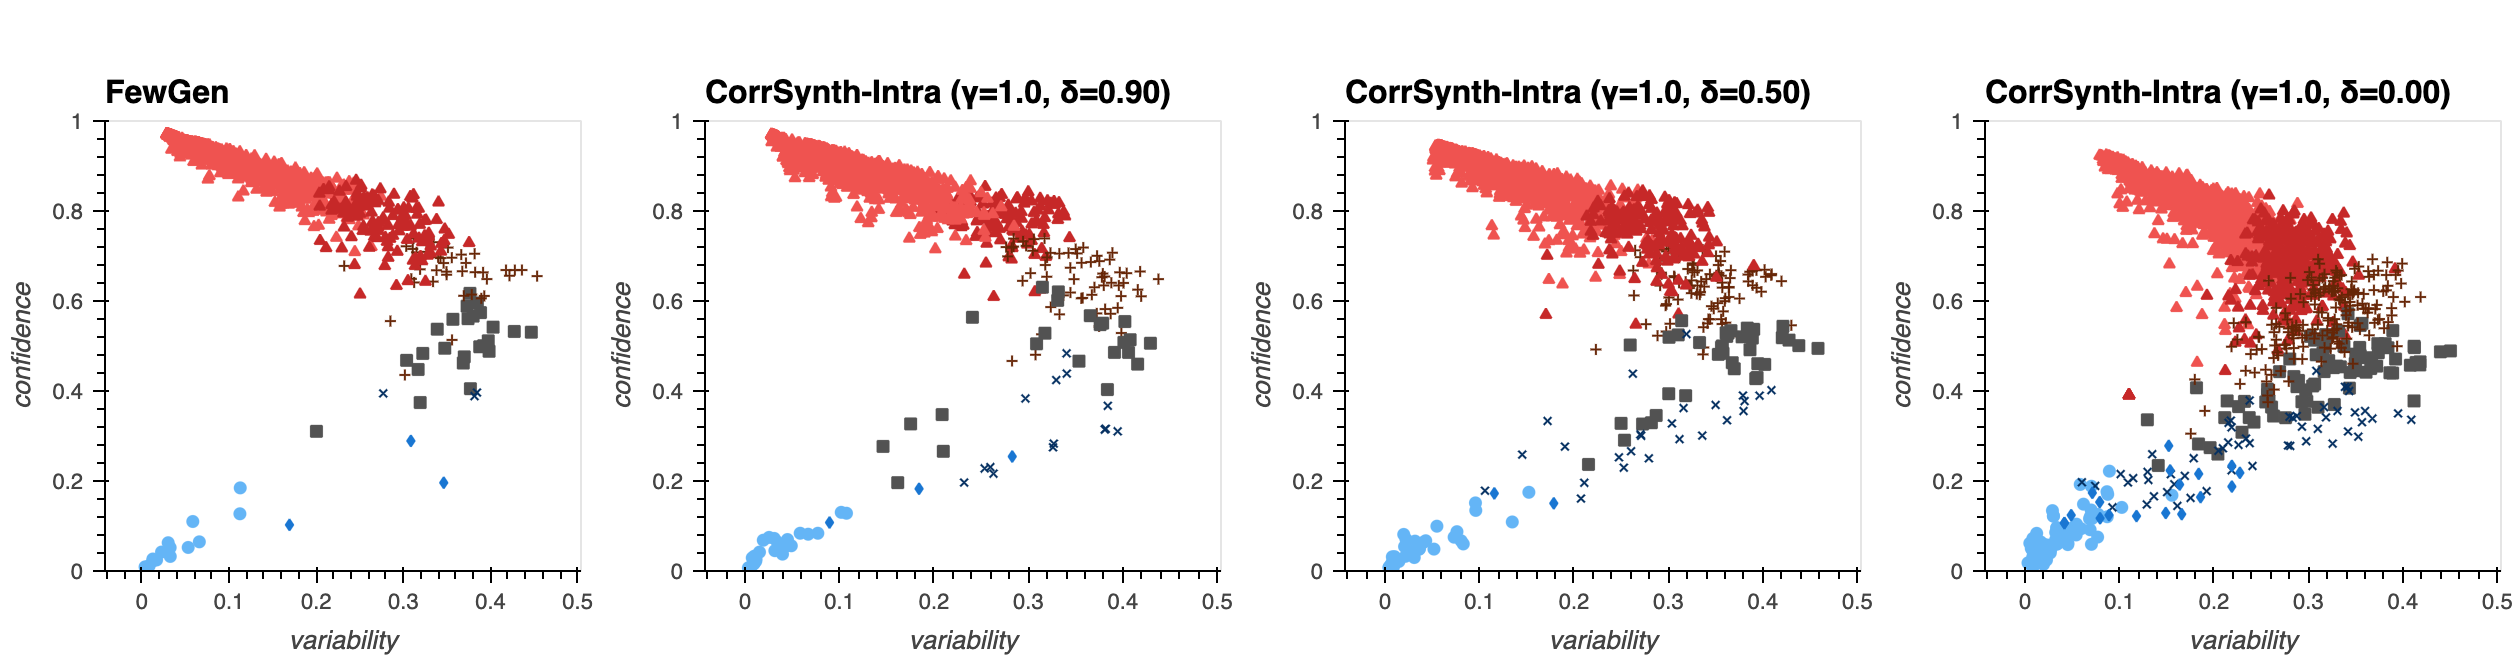
\includegraphics[width=\textwidth]{figure/carto_plots_v2.png}
\vspace{-0.5cm}
\caption{Datamaps for \DistilBERT\ training run on $2$K examples of \ToIHeadlines\ generated using \corrsyn-Intra using Phi-3-mini. \fewgen\ datamap is provided for reference.}
\vspace{-1em}
\label{fig:intra-label-carto}
\end{figure*}

\section{Analysis and Visualizations}
\label{sec:analysis}

\textbf{Effect of Intra-label and Cross-label contrasts:} Given the promising results of our method \corrsyn, we wanted to analyse and visualize the effect of varying Intra-label and cross-label contrasts upon the generations. For this, we obtain the average label-wise cosine similarities of the generations and plot them as heatmaps (see \autoref{fig:cosine}). We specifically study the behavior of our approach in multi-label setting upon \ToIHeadlines\ dataset to emphasize our results. In practice, we use the \texttt{all-mpnet-base-v2} model from SentenceTransformers library to obtain the text representations of each generation. Next, for generations each label $i$ and $j$ in the labelspace, we compute the pairwise cosine similarities of all generations corresponding to label $i$, to that of label $j$. The pairwise cosine similarities are then added and the mean label-wise similarity is computed. We hypothesize that in our approach (Hybrid \corrsyn), if the Intra label contrast is increased, then, within each class the generations should get further away so that the net cosine similarity within the class should reduce across all classes. As we can see in \autoref{fig:cosine_intra}, the diagonals become lighter as we go left to right. On the other hand, if the cross-label contrast is increased net separability between every pair of classes should increase. As expected, we can see in \autoref{fig:cosine_cross}, in the heatmaps the off-diagonal label similarities are becoming lighter as cross contrast is increased. 





\textbf{Effect of $\delta$:} To visualize the effect of varying $\delta$ on the generations obtained through \corrsyn, we plot 2-dimensional representations of the generations. We use Uniform Manifold Approximation and Projection (UMAP)~\cite{mcinnes2020umap} for Dimension Reduction\footnote{https://umap-learn.readthedocs.io/en/latest/} of text representations obtained using \texttt{all-mpnet-base-v2} model. As earlier, we perform this analysis in a multi-label setting with \ToIHeadlines. 

In \autoref{fig:intra_label_umaps}, we can see that as $\delta$ is reduced from $(0.9, 0.5, 0)$, the representations become more and more diffused with each other, leading to overlaps, making the student model hard to learn the decision boundary. For $\delta=0.9$, we can visualize the clusters containing data points from different labels are well-separated, which resonates with our best performing results as well. Note that overlapping/diffused datapoints could be indicators of mislabelled generations as well as hard negatives. 

We hypothesize that as we decrease delta from $0.9$, first we see an increase in hard negative generations than mislabeled generations, whereas after some threshold, the extent of mislabeled generations increase. Thus there is a sweet spot which provides good amount of hard examples with minimal number of wrong generations. We can see this effect in the corresponding cartography plots \cite{swayamdipta-etal-2020-dataset} in \autoref{fig:intra-label-carto} where as we go from left to right, the density of gray and blue points increase but blue points density increases more for much smaller delta than for gray points. The gray points here typically denote hard to learn examples, where as the blue one predominantly represent mislabeled example. These hard negative generations benefit the student model training. %We can see in the corresponding cartography plots in \autoref{fig:intra-label-carto}, we are able to generate more datapoints having low classification confidence and high variability, which in turn benefits the model during training.
\section{Related Work}
\textbf{Dataset synthesis using LLMs.} In recent years LLMs have exhibited strong generative capabilities \cite{NEURIPS2020_1457c0d6, Cobbe2021TrainingVT} to solve a diverse range of tasks. With well-designed prompts, large-scale LLMs have shown its notable zero-shot and few-shot learning ability \cite{shin-etal-2020-autoprompt, jiang-etal-2020-know, 10.1145/3411763.3451760}. 

More recently, these models have gained popularity in their superior ability to synthesize task-specific datasets \cite{Wang2021TowardsZL, Lee2021NeuralDA, kumar-etal-2020-data, puri-etal-2020-training, AnabyTavor2019DoNH}. LLMs such as GPT-3 \cite{wang-etal-2023-self-instruct, honovich-etal-2023-unnatural, west-etal-2022-symbolic} and chat-tuned models \cite{Yehudai2024GenieAH, yu2023large, wang-etal-2023-lets} have shown promising results on the task of generating synthetic data. Certain works like \citet{Meng2023TuningLM} fine-tune an LLM to generate NLU datasets, whereas our work is similar to \citet{schick-schutze-2021-generating,Meng2022GeneratingTD} which use frozen LLMs with task-dependent prompts to generate data, targeting text classification.

\textbf{Text classification dataset synthesis} employs class-specific prompts; previous studies explored zero-shot \cite{Ye2022ZeroGenEZ} and iterative few-shot prompting \cite{ye-etal-2022-progen}. However, only recently has the lack of diversity in synthetic classification datasets been recognized. \citet{yu2023large} advocated for using diverse prompts that explicitly introduce variations, such as subtopics and brands, resulting in more diverse conditioning. In contrast, our approach achieves diversity with a fixed prompt. \citet{divekar2024synthesizrr} employs retrieval augmentation to introduce variety into the dataset synthesis process by seeding the LLM with different content. However, the diversity here is constrained by the corpus availability, whereas our work improves diversity despite relying only on LLM parameters.

% \textbf{Retrieval-augmented Generation} bypasses numerous problems associated with generating solely from parametric memory, i.e. heightened bias towards “head” entities \cite{mallen-etal-2023-trust}, lower lexical diversity \cite{Holtzman2020The},  \cite{jentzsch-kersting-2023-chatgpt}, and hallucinated and confabulated information \cite{Zhang2023SirensSI}.  \cite{yu-etal-2023-regen} studied the retrieval-only setting for creation of topic and sentiment datasets. 

\textbf{Classifier-Free Guidance (CFG)} is a sampling technique introduced in diffusion literature~\cite{ho2021classifierfree} and later extended to autoregressive LLMs~\cite{sanchez2023stay}. CFG falls under general guidance based techniques, where a guidance distribution is used at inference to alter the sampling distribution towards the desired goal.In CFG, this guidance distribution is provided by the LLM itself but with a different prompt as described in \aref{sec:CFG}. Context-aware decoding~\citet{Shi2023TrustingYE} also uses the same formulation as CFG.

\textbf{Contrastive decoding (CD} refers to another family of guidance based methods that derive the guidance distribution from either a smaller LLM~\cite{o2023contrastive,li2023contrastive}, different layers of the same LLM~\cite{chuang2023dola,gera-etal-2023-benefits}. In all these methods from CFG to CD, the idea is essentially that to generate a sequence, a contrasting distribution is computed at inference. But different sequences are generated independently. In \corrsyn{}, although we borrow the general idea of a using a guidance-providing distribution at inference, the guidance distribution itself corresponds to a actual parallel generation providing both a) (anti-)correlation between multiple sequences as desired, b) compute efficiency. See \autoref{sec:method} and \autoref{sec:compare_cfg_corrsyn_app}.


\section{Conclusion}
In this work, we propose a novel technique \corrsyn\ which uses correlated sampling and intuition from classifier free guidance and contrastive decoding to generate strongly diverse datasets across a variety of tasks with good cross-label separations. We provide the mathematical intuition of our approach and back our theoretical discussion with empirical results. Our extensive experimentation across 4 datasets show the robustness of our approach in generating synthetic data. 

In the future, we would like to study the effect of including Intra-label contrasts while generating with the LLMs, and mixing up both cross-label and Intra-label contrasts (a hybrid approach) to see how the generations are affected with respect to both intrinsic and extrinsic evaluation.
\section{Limitations}
The scope of our experiments is restricted to a set of classification tasks over a few English domains of text. While we believe our approach can be applied to other languages, other domains, and tasks like question answering that go beyond classification, we have not validated this in this work. Furthermore, the scope of our formulation is restricted to supervised learning problems where there a well-defined or natural label space. Extensions to unsupervised tasks like datasets for pre-training is an interesting possibility to be explored. The introduction of new hyper-parameters in any method requires tuning, which increases costs. In our case a high value of $\delta$ with respect to the original guidance $\gamma$ (e.g. $\delta = 0.9*\gamma$, yields positive results for all guidance values). However, the tuning of the initial guidance parameter was subject to a heuristic search. Finally, our approach performs modifications to the generation process by performing correlated sampling in the logits space. This makes our approach infeasible to use with API-only teacher LMs such as GPT-4, Claude, Gemini, etc. 



% Bibliography entries for the entire Anthology, followed by custom entries
%\bibliography{anthology,custom}
% Custom bibliography entries only
\bibliography{custom, refs}

\appendix
\section{Risks}

Although the main goal of our work is to improve text classification, our use of LLMs to generate examples does carry some conceptual risks. By generating news headlines and reviews to train classifiers on, we run the risk of generating fake news and other harmful content. However, we believe this risk is mitigated by the fact that the final outcome of our system is a classifier: classification models have relatively constrained failure modes (misclassification) compared to text generation models that can mislead users. Furthermore, we do not believe our approach uniquely advances the generation of content like fake news or reviews; our advances are largely orthogonal to the technology that brings such risks.

\section{Ablation: without in-context learning}
\label{app:zeroshot}

We explore the performance from \fewgen{} and \corrsyn{} in the absence of in-context examples. Recall that in \autoref{tab:accuracy-diversity-icl}, we used 3 in-context examples selected at random from a small seed set of 50 per class (for multiclass tasks) and 100 per class (for binary tasks). 

In this ablation, we remove this dependence completely and do not pass any in-context examples; thus, the next-token distribution is the same for each batch of contrasting terms we generate, and the variation in generations is solely a function of the top-p sampling, rather than a change to the next-token distribution which was induced due to in-context examples in the prompt.

In \autoref{tab:accuracy-diversity-zeroshot}, we observe that once again, \corrsyn{} consistently demonstrates superior diversity and accuracy compared to \fewgen. However, we note that in-context examples do improve all metrics, and thus we recommend including them in the base prompt.
% Please add the following required packages to your document preamble:
% \usepackage{booktabs}
% \usepackage{multirow}
\begin{table*}[h]
\centering
\begin{tabular}{
L{65pt}
% h
c % Teacher
C{16pt} % AG 
C{17pt} % ToI
C{18pt} % Humor
C{24pt} % IMDb
C{20pt} % Avg
|C{16pt} % AG 
C{17pt} % ToI
C{18pt} % Humor
C{24pt} % IMDb
C{20pt} % Avg
}

\toprule
\multirow{2}{*}{\textbf{Method}}   
& \multirow{2}{*}{\textbf{Teacher}} %\multicolumn{1}{h}{\multirow{2}{*}{\textbf{Params}}}
% &  %\multicolumn{1}{C{26pt}}{\multirow{2}{*}{\textbf{Teacher}}}
& \multicolumn{4}{c}{\textbf{Accuracy \higherbetter}}
& \multirow{2}{*}{\textbf{Avg.}}
& \multicolumn{4}{c}{\textbf{MAUVE \higherbetter}}
& \multirow{2}{*}{\textbf{Avg.}}
\\ 
\cmidrule(l){3-6}         
\cmidrule(l){8-11}         
% & 
& \textbf{LM} % \multicolumn{1}{c}{\textbf{LM}}
& \textbf{\AG} % AG Accuracy
& \textbf{\ToI} % ToI Accuracy
& \textbf{\Hum} % Hum Accuracy
& \textbf{\IMDb} % IMDb Accuracy
&
& \textbf{\AG} % AG Mauve
& \textbf{\ToI} % ToI Mauve
& \textbf{\Hum} % Hum Mauve
& \textbf{\IMDb} % IMDb Mauve
&
\\ 
\midrule
\gold          
% & %\multicolumn{1}{c}{-}                
& \multicolumn{1}{c}{-}                
& 91.4         & 78.9         & 92.9          & 91.4 & 88.7
& -         & -         & -          & - & -
\\ 
\midrule
%% Zero-shot
\multicolumn{12}{c}{\underline{\textsc{Zero-shot}}} \\
[0.5ex]
\fewgen 
% & % \multicolumn{1}{c}{-} 
& \multicolumn{1}{c}{\PhiMini}
& 70.3         & 53.4         & \textbf{69.0}          & 71.9 & 66.2
& 55.9         & 51.2         & 56.4          & 52.7 & 54.1
\\ 
\fewgen 
% & % \multicolumn{1}{c}{-} 
& \multicolumn{1}{c}{\Mixtral}          
& 74.0         & 51.1         & 49.1          & 64.3 & 58.1
& 50.6         & 50.0         & 52.4          & 54.1 & 51.8
\\ 
[1.0ex]

\corrsynreallyshort-Intra 
% & % \multicolumn{1}{c}{-} 
& \multicolumn{1}{c}{\PhiMini}
& 68.5         & 57.5         & 65.8          & 76.8 & 67.2
& \textbf{59.4}         & 53.7         & 62.0          & 58.4 & 58.4
\\ 
\corrsynreallyshort-Hybrid 
% & % \multicolumn{1}{c}{-} 
& \multicolumn{1}{c}{\PhiMini}
& \textbf{85.1}         & \textbf{59.3}         & 65.3          & 78.0 & \textbf{71.9}
& 57.8         & \textbf{56.7}        & \textbf{63.3}          & \textbf{58.5} & \textbf{59.1}
\\ 
[0.5ex]

\corrsynreallyshort-Intra 
% & % \multicolumn{1}{c}{-} 
& \multicolumn{1}{c}{\Mixtral}
& 74.4         & 54.5         & 52.2          & 78.1 & 64.8
& 53.6         & 50.8         & 52.4          & 55.7 & 53.1
\\  
\corrsynreallyshort-Hybrid 
% & % \multicolumn{1}{c}{-} 
& \multicolumn{1}{c}{\Mixtral}
& 73.8         & 55.0         & 58.6           & \textbf{78.7} & 66.5
& 54.1         & 51.2         & 52.6          & 56.7 & 53.7
\\ 
[1.0ex]
\toprule
\multirow{2}{*}{\textbf{Method}}   
& \multirow{2}{*}{\textbf{Teacher}} %\multicolumn{1}{h}{\multirow{2}{*}{\textbf{Params}}}
% &  %\multicolumn{1}{C{26pt}}{\multirow{2}{*}{\textbf{Teacher}}}
& \multicolumn{4}{c}{\textbf{Self-BLEU-5 \lowerbetter}}
& \multirow{2}{*}{\textbf{Avg.}}
& \multicolumn{4}{c}{\textbf{Entity-Entropy \higherbetter}}     
& \multirow{2}{*}{\textbf{Avg.}}
\\
\cmidrule(l){3-6}         
\cmidrule(l){8-11}         
% & 
& \textbf{LM} % \multicolumn{1}{c}{\textbf{LM}}
& \textbf{\AG} % AG Accuracy
& \textbf{\ToI} % ToI Accuracy
& \textbf{\Hum} % Hum Accuracy
& \textbf{\IMDb} % IMDb Accuracy
&
& \textbf{\AG} % AG Mauve
& \textbf{\ToI} % ToI Mauve
& \textbf{\Hum} % Hum Mauve
& \textbf{\IMDb} % IMDb Mauve
&
\\
\midrule
\gold          
% & %\multicolumn{1}{c}{-}                
& \multicolumn{1}{c}{-}                
& 17.1         & 7.9         & 19.8          & 27.9 & 18.2
& 6.6         & 6.1         & 5.1          & 7.5 & 6.3
\\ 
\midrule
\multicolumn{12}{c}{\underline{\textsc{Zero-shot}}} \\
[0.5ex]
\fewgen 
% & % \multicolumn{1}{c}{-} 
& \multicolumn{1}{c}{\PhiMini}
& 67.2         & 58.7         & 62.9          & 76.5 & 66.3
& 3.5         & 4.6         & 3.8          & 3.1 & 3.8
\\ 
\fewgen 
% & % \multicolumn{1}{c}{-} 
& \multicolumn{1}{c}{\Mixtral}
& 90.1         & 97.3         & 93.4          & 94.7 & 93.9
& 2.3         & 2.4         & 1.4          & 1.7 & 1.9
\\ 
[1.0ex]

\corrsynreallyshort-Intra 
% & % \multicolumn{1}{c}{-} 
& \multicolumn{1}{c}{\PhiMini}
& 34.8         & 28.8         & 33.8          & 51.0 & 37.1
& 4.9         & 4.8         & 4.5          & 4.4 & 4.6
\\ 
\corrsynreallyshort-Hybrid 
% & % \multicolumn{1}{c}{-} 
& \multicolumn{1}{c}{\PhiMini}
& \textbf{33.2}         & \textbf{27.8}         & \textbf{31.9}          & \textbf{46.6} & \textbf{34.9}
& \textbf{5.3}         & \textbf{5.1}         & \textbf{4.6}          & \textbf{4.8} & \textbf{5.0}
\\ 
[0.5ex]
\corrsynreallyshort-Intra 
% & % \multicolumn{1}{c}{-} 
& \multicolumn{1}{c}{\Mixtral}
& 78.1         & 87.3         & 76.9          & 84.7 & 81.8
& 3.1         & 3.4         & 2.5          & 2.8 & 3.0
\\  
\corrsynreallyshort-Hybrid 
% & % \multicolumn{1}{c}{-} 
& \multicolumn{1}{c}{\Mixtral}
& 77.4         & 86.0         & 75.0          & 81.3 & 79.9
& 3.3         & 3.3         & 2.7           & 3.1 & 3.1
\\ 
\bottomrule
\end{tabular}
\caption{
Evaluation of intrinsic dataset quality and \DistilBERT\ student model fine-tuned on real and synthetic datasets using zero-shot generation. We report mean accuracy numbers across 5 runs. %Hyphens indicate datasets have not been released by authors. 
}
\label{tab:accuracy-diversity-zeroshot}
\end{table*}

\section{\fewgen{}}% \ad{Don't add FewGen, start from CFG directly.}
\label{sec:fewgen}
Let us consider the case of binary classification with labels $\{0,1\}$ and corresponding verbalization $\{\mathbf{y}_0,\mathbf{y}_1\}$. \fewgen{}~\cite{gpt3} is a standard approach to generate an instance $\mathbf{x}$ for a label $\mathbf{y}$: construct a prompt $\Prompt$ that has some description of the classification task, few ICL example generations, optional instance attributes and the choice of label $\mathbf{y}\in\{\mathbf{y}_0,\mathbf{y}_1\}$, and task the LLM to generate $x$. For brevity, we only keep the dependence of $\Prompt$ on $\mathbf{y}$ and use the notation $\Prompt(\mathbf{y})$ to denote the \textit{prompt tokens}. Let $\mP$ denote the auto-regressive LLM probability distribution with vocabulary $\cV$. An instance corresponding to label $\mathbf{y}$ is sampled in \fewgen{} as 
\begin{equation}
\label{eq:std_sample}
    \mathbf{x}=(x_1,\cdots,x_n)\distas{}\mP(\cdot|\Prompt(\mathbf{y}))
\end{equation}


\section{CFG}
\label{sec:CFG}
In CFG decoding~\cite{sanchez2023stay}, output token distribution is tilted in order to ensure that the LLM generations satisfy a particular condition.  In particular, we construct a \textit{contrastive prompt} $\widebar{\Prompt}$, and choose a guidance strength $\gamma>0$. Then instead of \eqref{eq:std_sample}, $\mathbf{x}$ is sampled using a titled distribution $\tilde \mP$ where
\begin{align}
    \tilde \mP(\cdot)& \propto  \frac{\mP(\cdot|\Prompt(\mathbf{y}))^{\gamma+1}}{\mP(\cdot|\widebar{\Prompt})^{\gamma}}\nonumber \\
    &=\mP(\cdot|\Prompt(\mathbf{y}))\left[\frac{\mP(\cdot|\Prompt(\mathbf{y}))}{\mP(\cdot|\widebar{\Prompt})}\right]^\gamma\label{eq:2cfg_seq}
\end{align}
Suppose we choose $\widebar{\Prompt}=\Prompt(\bar{\mathbf{y}})$, the prompt corresponding to the complementary label $\bar{\mathbf{y}}$ of $\mathbf{y}$ (or it could be any other label different from $\mathbf{y}$ in case of multiclass scenario). Then in the above equation, we are up-weighing the sequences that likely under $\Prompt(\mathbf{y})$ but unlikely under $\bar{\mathbf{y}}$ using the ratio of the two probabilities. This is supposed to move the generations away from the complementary label $\bar{\mathbf{y}}$. Writing in terms of tokens, we sample the $i$-th token $x_i$ as follows
\begin{equation}
    \label{eq:2cfg-ar}
    x_i\distas{}\tilde \mP(\cdot|\mathbf{x}_{<i}) \propto \frac{\mP(\cdot|\Prompt(\mathbf{y}),\mathbf{x}_{<i})^{\gamma+1}}{\mP(\cdot|\Prompt(\mathbf{\bar{\mathbf{y}}}),\mathbf{x}_{<i})^{\gamma}}
\end{equation}

\paragraph{Drawbacks:} We find two drawbacks in CFG:
\begin{enumerate}
    \item In equation \eqref{eq:2cfg-ar}, the same $\mathbf{x}_{<i}$ is fed as a continuation from both prompts $\Prompt(y)$ and $\Prompt(\mathbf{\bar{\mathbf{y}}})$. We posit that this leads to decrease in the effect on guidance as more tokens are generated. This is because even the generation $\mathbf{x}$ is expected to be more faithful to $\Prompt(\mathbf{y})$ than to $\Prompt(\mathbf{\bar{\mathbf{y}}})$. So even though $\Prompt(\mathbf{\bar{\mathbf{y}}})$ is sort of opposite to $\Prompt(\mathbf{y})$, feeding in the generations that are faithful to the latter would move the token distributions in the denominator closer to the numerator. This is shown in \autoref{fig:cfg_vs_corrsynth}.
    \item Only a single sequence is generated at the cost of increase in number of forward passes of the model by two-fold. So a natural $K$-way extension for $K$-class classification would incur $K^2$ forward passes through the model per token for generating a single token for each of the $K$-classes. 
\end{enumerate}


% % Please add the following required packages to your document preamble:
% \usepackage{booktabs}
% \usepackage{multirow}
\begin{table*}[h]
\centering
\begin{tabular}{
L{70pt}
% h
c % Teacher
C{18pt} % AG 
C{18pt} % ToI
C{18pt} % Humor
C{24pt} % IMDb
C{20pt} % Avg
| C{18pt} % AG 
C{18pt} % ToI
C{18pt} % Humor
C{24pt} % IMDb
C{20pt} % Avg
}

\toprule
\multirow{2}{*}{\textbf{Method}}   
& \multirow{2}{*}{\textbf{Teacher}} %\multicolumn{1}{h}{\multirow{2}{*}{\textbf{Params}}}
% &  %\multicolumn{1}{C{26pt}}{\multirow{2}{*}{\textbf{Teacher}}}
& \multicolumn{4}{c}{\textbf{Self-BLEU-5 \lowerbetter}}
& \multirow{2}{*}{\textbf{Avg.}}
& \multicolumn{4}{c}{\textbf{Entity-Entropy \higherbetter}}     
& \multirow{2}{*}{\textbf{Avg.}}
\\ 
\cmidrule(l){3-6}         
\cmidrule(l){8-11}         
% & 
& \textbf{LM} % \multicolumn{1}{c}{\textbf{LM}}
& \textbf{\AG} % AG Accuracy
& \textbf{\ToI} % ToI Accuracy
& \textbf{\Hum} % Hum Accuracy
& \textbf{\IMDb} % IMDb Accuracy
& 
& \textbf{\AG} % AG Mauve
& \textbf{\ToI} % ToI Mauve
& \textbf{\Hum} % Hum Mauve
& \textbf{\IMDb} % IMDb Mauve
&
\\ 
\midrule
\gold          
% & %\multicolumn{1}{c}{-}                
& \multicolumn{1}{c}{-}                
& 17.1         & 7.9         & 19.8          & 27.9 & 18.2
& 6.6         & 6.1         & 5.1          & 7.5 & 6.3
\\ 
\midrule
%% Zero-shot
\multicolumn{12}{c}{\underline{\textsc{Zero-shot}}}  \\
[0.5ex]
% \AttrPrompt 
% % & %\multicolumn{1}{c}{-} 
% & \multicolumn{1}{c}{\ChatGPTShort}     
% & 91.3         & 94.5         & 91.4          & 91.4 & -
% & 91.3         & 94.5         & 91.4          & 91.4 & -
% \\ 
% [0.5ex]
\fewgen 
% & % \multicolumn{1}{c}{-} 
& \multicolumn{1}{c}{Phi-3 mini}          
& 67.2         & 58.7         & 62.9          & 76.5 & 66.3
& 3.5         & 4.6         & 3.8          & 3.1 & 3.8
\\ 
\fewgen 
% & % \multicolumn{1}{c}{-} 
& \multicolumn{1}{c}{Mixtral}          
& 90.1         & 97.3         & 93.4          & 94.7 & 93.9
& 2.3         & 2.4         & 1.4          & 1.7 & 1.9
\\ 
[1.0ex]
% \oursshort & \multicolumn{1}{c}{-}  & \multicolumn{1}{c}{Phi-3 mini}          
% & 91.3         & 94.5         & 91.4          & 91.4
% & 91.3         & 94.5         & 91.4          & 91.4
% \\ 
% \oursshort & \multicolumn{1}{c}{-} & \multicolumn{1}{c}{Mixtral}          
% & 91.3         & 94.5         & 91.4          & 91.4
% & 91.3         & 94.5         & 91.4          & 91.4
% \\ 
% [0.5ex]
% \corrsynreallyshort-Cross 
% % & % \multicolumn{1}{c}{-} 
% & \multicolumn{1}{c}{Phi-3 mini}          
% & 91.3         & 94.5         & 91.4          & 91.4 & -
% & 91.3         & 94.5         & 91.4          & 91.4 & -
% \\ 
\corrsynreallyshort-Intra 
% & % \multicolumn{1}{c}{-} 
& \multicolumn{1}{c}{Phi-3 mini}          
& 34.8         & 28.8         & 33.8          & 51.0 & 37.1
& 4.9         & 4.8         & 4.5          & 4.4 & 4.6
\\ 
\corrsynreallyshort-Hybrid 
% & % \multicolumn{1}{c}{-} 
& \multicolumn{1}{c}{Phi-3 mini}          
& \textbf{33.2}         & \textbf{27.8}         & \textbf{31.9}          & \textbf{46.6} & \textbf{34.9}
& \textbf{5.3}         & \textbf{5.1}         & \textbf{4.6}          & \textbf{4.8} & \textbf{5.0}
\\ 
[0.5ex]
% \corrsynreallyshort-Cross 
% % & % \multicolumn{1}{c}{-} 
% & \multicolumn{1}{c}{Mixtral}          
% & 91.3         & 94.5         & 91.4          & 91.4 & -
% & 91.3         & 94.5         & 91.4          & 91.4 & -
% \\ 
\corrsynreallyshort-Intra 
% & % \multicolumn{1}{c}{-} 
& \multicolumn{1}{c}{Mixtral}          
& 78.1         & 87.3         & 76.9          & 84.7 & 81.8
& 3.1         & 3.4         & 2.5          & 2.8 & 3.0
\\  
\corrsynreallyshort-Hybrid 
% & % \multicolumn{1}{c}{-} 
& \multicolumn{1}{c}{Mixtral}          
& 77.4         & 86.0         & 75.0          & 81.3 & 79.9
& 3.3         & 3.3         & 2.7           & 3.1 & 3.1
\\ 
\midrule
%% Few-shot (Human seed)
%
%
%
%
%
%
%
%
%
%
%
%
%
\multicolumn{12}{c}{\underline{\textsc{In-Context Learning}}} \\
[0.5ex]
\fewgen 
% & % \multicolumn{1}{c}{-} 
& \multicolumn{1}{c}{Phi-3 mini}          
& 33.9         & 15.3         & 39.9          & 57.7 & 36.7
& 6.6         & 6.3         & 4.3          & 5.3 & 5.6
\\ 
\fewgen 
% & % \multicolumn{1}{c}{-} 
& \multicolumn{1}{c}{Mixtral}          
& 39.4         & 37.9         & 64.6          & 66.5 & 52.1
& 5.9         & 5.2         & 3.6         & 5.2 & 5.0
\\ 
[1.0ex]
% \oursshort & \multicolumn{1}{c}{-}  & \multicolumn{1}{c}{Phi-3 mini}          
% & 91.3         & 94.5         & 91.4          & 91.4
% & 91.3         & 94.5         & 91.4          & 91.4
% \\ 
% \oursshort & \multicolumn{1}{c}{-} & \multicolumn{1}{c}{Mixtral}          
% & 91.3         & 94.5         & 91.4          & 91.4
% & 91.3         & 94.5         & 91.4          & 91.4
% \\ 
% [0.5ex]
% \corrsynreallyshort-Cross 
% % & % \multicolumn{1}{c}{-} 
% & \multicolumn{1}{c}{Phi-3 mini}          
% & 91.3         & 94.5         & 91.4          & 91.4 & -
% & 91.3         & 94.5         & 91.4          & 91.4 & -
% \\ 
\corrsynreallyshort-Intra 
% & % \multicolumn{1}{c}{-} 
& \multicolumn{1}{c}{Phi-3 mini}          
& 13.1         & 9.0         & 23.5          & 24.9 & 17.6
& \textbf{7.4}         & \textbf{6.9}         & \textbf{4.9}          & \textbf{6.5} & \textbf{6.4}
\\ 
\corrsynreallyshort-Hybrid 
% & % \multicolumn{1}{c}{-} 
& \multicolumn{1}{c}{Phi-3 mini}          
& \textbf{12.1}         & \textbf{8.7}         & \textbf{22.8}          & \textbf{19.2} & \textbf{15.7}
& \textbf{7.4}         & \textbf{6.9}        & 4.8          & 6.4 & \textbf{6.4}
\\ 
[0.5ex]
% \corrsynreallyshort-Cross 
% % & % \multicolumn{1}{c}{-} 
% & \multicolumn{1}{c}{Mixtral}          
% & 91.3         & 94.5         & 91.4          & 91.4 & -
% & 91.3         & 94.5         & 91.4          & 91.4 & -
% \\ 
\corrsynreallyshort-Intra 
% & % \multicolumn{1}{c}{-} 
& \multicolumn{1}{c}{Mixtral}          
& 18.9         & 17.6         & 45.3          & 33.0 & 28.7
& 6.3          & 5.7         & 3.7          & 6.0 & 5.4
\\  
\corrsynreallyshort-Hybrid 
% & % \multicolumn{1}{c}{-} 
& \multicolumn{1}{c}{Mixtral}          
& 17.5         & 18.4         & 41.4          & 27.4 & 26.2
& 6.5         & 5.6         & 4.1         & 6.4 & 5.7
\\ 
\bottomrule
\end{tabular}
\caption{
Evaluation of diversity metrics on real and synthetic datasets. In the bottom half (in-context learning) when generating each instance, we select 3 in-context examples at random to prime the LLM's next-token distribution before sampling continuations.
}
\label{tab:bleu-entropy}
\end{table*}

\section{Geometric mean interpretation and $K$-class \corrsyn{}}
\label{sec:geometric}
To gain intuition on \corrsyn{}, we present an interpretation of it using geometric mean. We continue to use the notation from \ref{sec:M-corrsyn}. First we present the uniform contrastive guidance described briefly in the main paper.

\subsection{Uniform contrastive guidance}

\label{sec:app_unif_guidance}
We set a parameter $\delta$ that controls the total amount of contrast guidance: for each $m$, $\sum_n \gamma_{m,n}=\gamma-\delta$. 
At step $i$, let the active set $\cS_{i}=\{m\in[M]:x_{m,i-1}\neq \eos\}\}$ which captures the sequences which have not yet hit the EOS token. Let $M_{i,active}=|\cS_{i}|$ denote the number of such sequences. Then in uniform contrastive guidance we set 
$$\gamma_{m,n}=\begin{cases} \frac{\gamma-\delta}{M_{i,active}-1}&,\, m,n\in\cS_i\\
 0&,\, \mathrm{otherwise}\end{cases}$$
at stage/token $i$ (dependence of $\gamma_{m,n}$ on $i$ is suppressed). 
Thus equation \eqref{eq:M-Corr-1} becomes
\begin{align}
    x_{m,i}&\distas{} \tilde \mP_{m,i}(\cdot)\nonumber\\
    &\propto \frac{\mP(\cdot| \Prompt_m,\mbf{x}_{m,<i})^{\gamma}}{\prod_{\substack{n\in \cS_i \\n\neq  m}}\mP(\cdot| \Prompt_n,\mbf{x}_{n,<i})^{\frac{\gamma-\delta}{M_{i,active}-1}}}\label{eq:M-Corr-2}
\end{align}

\subsection{Geometric mean}
Let us assume that $S_i=[M]$ and hence $M_{i,active}=M$. Further let $\delta=0$. Recall that the geometric mean of $n$ non-negative reals $\{\alpha_1,\cdots,\alpha_n\}$ is given by
\begin{equation}
    GM(\{\alpha_i:i\in [n]\})=\left(\prod_{i=1}^n\alpha_i\right)^{\frac{1}{n}}
\end{equation}
Analogously we can define the geometric mean of $M$ probability distributions in a point-wise manner. Thus we can write \eqref{eq:M-Corr-2} as
\begin{align}
     &x_{m,i}\distas{}\tilde \mP_{m,i}(\cdot)\nonumber\\
    &\propto \frac{\mP(\cdot| \Prompt_m,\mbf{x}_{m,<i})^{\gamma}}{GM\left(\{\mP(\cdot| \Prompt_n,\mbf{x}_{n,<i}):n\in \cS_i, n\neq m\}\right)^{\gamma}}\label{eq:M-Corr-3}
\end{align}
 Thus, in \corrsyn, the contrasting guidance signal is provided by a \textit{geometric ensemble} of token distributions obtained from contrasting prompts as well as corresponding contrasting sequences. We expect that this geometric ensemble contrast, when $M\gg 2$, to average out the signal from the contrast and mitigate the issue of non alignment of words or entities between sequences. 

 \subsection{\corrsyn{} for $K$-class data generation}
 \label{sec:K-corrsyn}
 In this section we describe how \corrsyn{} is applied to generate data for $K$-class text classification problem. Recall that in $K$-class classification problem over $\cX\times\cY$ we have classes $[K]$ with label verbalizations $\{\mbf{y}_1,\cdots,\mbf{y}_K\}$. To generates instances for each class, we create prompts as follows. Let $R\in\mathbb{N}$ be the repeat factor. For each class $\mbf{y}$ consider the, possibly empty, ICL examples sets $\cI_{\mbf{y},r}\subset \cX\times\cY$ for $r\in [R]$ which contain positive examples for $\mbf{y}$. We construct a set of $K\cdot R$ prompts $\{\Prompt_{k,r}:k\in[K],r\in[R]\}$ where $\Prompt_{k,r}=\Prompt(\mbf{y}_k,\cI_{\mbf{y}_k,r})$ is a prompt that asks the LLM to generate instances for the class ${\mbf{y_k}}$ and includes ICL examples in $\cI_{\mbf{y}_k,r}$. For brevity, we assume that no sequence hits $\eos$ until some pre-set max number of tokens has been reached. There are a couple of ways in which \corrsyn{} can be used. Here we describe just one of the ways.%We describe two ways in which \corrsyn{} can be used.

 \subsubsection{Cross-label \corrsyn{}}
Here we contrast the instance for a label $\mbf{y_k}$ with instances of all the other labels $\mbf{y}_{k'}$ where $k'\neq k$. Thus, assuming uniform contrastive guidance~\ref{sec:unif_guidance}, we generate instances $\{\mbf{x}_{k,r}:k\in[K], r\in[R]\}$ together in \textit{lockstep} as follows. At stage/token $i$ we have for every $k\in[k]$ and $r\in [R]$
 % \begin{align}
 % \begin{aligned}
 %      & x_{k,r,i}\distas{} \tilde \mP_{k,r,i}(\cdot) \\
 %      &\propto \frac{\mP(\cdot| \Prompt_{k,r},\mbf{x}_{k,r,<i})^{\gamma}}{GM\left(\left\{\mP(\cdot| \Prompt_{k',r'},\mbf{x}_{k',r',<i})\right\}_{\substack {k'\neq k\\ r'\in[R]}}\right)^{\gamma-\delta}}\\
 %     &= \frac{\mP(\cdot| \Prompt(\mbf{y}_k,\cI_{\mbf{y}_k,r}),\mbf{x}_{k,r,<i})^{\gamma}}{GM\left(\left\{\mP(\cdot| \Prompt(\mbf{y}_{k'},\cI_{\mbf{y}_{k'},r'}),\mbf{x}_{k',r',<i})\right\}_{\substack {k'\neq k\\ r'\in[R]}}\right)^{\gamma-\delta}}\label{eq:K-Corr-cross-1}
 % \end{aligned}
 % \end{align}
 \begin{align}
 \begin{aligned}
      & x_{k,r,i}\distas{} \tilde \mP_{k,r,i}(\cdot) \\
      &\propto \frac{\mP(\cdot| \Prompt_{k,r},\mbf{x}_{k,r,<i})^{\gamma}}{GM\left(\left\{\mP(\cdot| \Prompt_{k',r'},\mbf{x}_{k',r',<i})\right\}_{\substack {k'\neq k\\ r'\in[R]}}\right)^{\gamma-\delta}}\label{eq:K-Corr-cross-1}
 \end{aligned}
 \end{align}
 \paragraph{Effect of repeat factor:} We include repeat factor because it will increase the number of contrast terms for taking the geometric mean. We expect that this would provide improved averaging and reduces the noise due to potential misalignment.% \sk{What do experiments show?}


 \subsubsection{Hybrid \corrsyn{}}
%  That is, we fix two targets $\gamma_{intra}$ and $\gamma_{cross}$, and for any $k$, $r$, letting $m=(k-1)R+r$, we choose $\gamma_{m,n}$ such that
% \begin{align}
%     \gamma_{intra}&=\sum_{\substack{n\in\{(k-1)R+r':\\r'\neq r\}}}\gamma_{m,n},\,\forall k,r\\
%     \gamma_{cross}&=\sum_{\substack{n\in\{(k'-1)R+r':\\ r'\in[R],k'\neq k\}}}\gamma_{m,n},\,\forall k,r
% \end{align}
% Then we uniformly split the target guidances $\gamma_{intra}$ and $\gamma_{cross}$ in respective groups. More details of $K$-class \corrsyn{} is given in appendix~\ref{sec:K-corrsyn}

 In the hybrid approach, we contrast the instance $\mbf{x}_{k,r}$ for a label $\mbf{y}_k$ with instances $\mbf{x}_{k,r'}$ of the same label (but with different repeat $r'\neq r$), as well as instances $\mbf{x}_{k',r'}$ for all the other labels (where $k'\neq k$, and $r'\in [R]$). We separately set the target guidance for each of the cross and intra label terms. That is, we fix two targets $\gamma_{intra}$ and $\gamma_{cross}$. Within each group we use uniform contrastive guidance from \ref{sec:unif_guidance}. The instances are generated as follows. At stage/token $i$ we have for every $k\in[k]$ and $r\in [R]$
 
 \begin{align}
 \begin{aligned}
      x_{k,r,i}&\distas{}\tilde \mP_{k,r,i}(\cdot) \\
      &\propto \frac{\mP(\cdot| \Prompt_{k,r},\mbf{x}_{k,r,<i})^{\gamma}}{GM_{intra}^{\gamma_{intra}}\cdot GM_{cross}^{\gamma_{cross}}}\label{eq:K-Corr-hybrid-1}
 \end{aligned}
 \end{align}

 where 
 \begin{align}
 \begin{aligned}
     &GM_{intra}=\\
     &GM\left(\left\{\mP(\cdot| \Prompt_{k,r'},\mbf{x}_{k,r',<i})\right\}_{\substack {r'\neq r}}\right)\\
     &GM_{cross}=\\
     &GM\left(\left\{\mP(\cdot| \Prompt_{k',r'},\mbf{x}_{k',r',<i})\right\}_{\substack {k'\neq k\\ r'\in[R]}}\right)
\end{aligned}
 \end{align}
 
As seen from the above display, the first term in the denominator gives contrast signal from generations with the class, in order to get good intra-label diversity. While the second term gives contrast signal from other classes and hence serves to increase class separation. 

\subsection{\corrsyn{} in logits space}
\label{sec:logit_corrsyn}
 Although the \corrsyn{} method described using LLM token probability distribution, it is implemented in the space of model outputs, i.e., logits. That is, the next-token distribution is obtained by first computing the next-token logits using logits-space \corrsyn{} as described below. It is equivalent\footnote{This is not fully equivalent to probability space version since taking logarithm gives us log-probabilities which are normalized version of logits. Experimentally we have not found significant impact of this normalization.} to taking logarithm of the \corrsyn{} equations, for e.g., \eqref{eq:K-Corr-cross-1} and \eqref{eq:K-Corr-hybrid-1}. For instance, in the cross-label version, the next token logits $\tilde \lg_{k,r,i}(\cdot)$ is given by
  \begin{align}
 \begin{aligned}
      \widetilde \lg_{k,r,i}(\cdot) =&\gamma\lg(\cdot| \Prompt_{k,r},\mbf{x}_{k,r,<i}) -\\
      &\frac{\gamma-\delta}{M-1}\sum_{\substack {k'\neq k\\ r'\in[R]}}\lg(\cdot| \Prompt_{k',r'},\mbf{x}_{k',r',<i}) \label{eq:K-Corr-cross-logit-1}
 \end{aligned}
 \end{align}
Similarly, we can derive the logit version for the hybrid \corrsyn{}

\subsection{\corrsyn{} with Plausibility constraint}
\label{sec:plaus}
The contrast terms in \corrsyn{} could sometimes up weigh some irrelevant tokens that are not plausible at all for the prompt/label under consideration. We borrow the idea of plausibility constraint from \cite{li2023contrastive, o2023contrastive} to limit the space of tokens that can up weighted by contrast terms. For the generation $\mbf{x}_{k,r}$ we consider the plausible set $\cT_{k,r,i}(\alpha)$, as a function of the plausibility constraint $\alpha\in [0,1]$, defined as 
\begin{align}
    \cT_{k,r,i}(\alpha)=&\left\{w\in\cV: P(w|\Prompt_{k,r},\mbf{x}_{k,r,<i})\geq \right.\nonumber\\
    &\left.\alpha \max_u P(u|\Prompt_{k,r},\mbf{x}_{k,r,<i})\right\}\label{eq:plaus_set}
\end{align}
i.e., at stage/token $i$, it is all those plausible tokens which have a token probability of at least $\alpha$ times the maximum token probability. So incorporating the plausibility constraint into  \corrsyn{} would result in the following logit function for $\mbf{x}_{k,r}$ in cross-label version
\begin{align}
 &\widetilde \lg^{\alpha}_{k,r,i}(w) = \begin{cases}
    \widetilde\lg_{k,r,i}(w), & w\in \cT_{k,r,i}(\alpha)\\
    -\infty, & \mathrm{otherwise}
\end{cases} \label{eq:K-Corr-cross-logit-plaus-1}
\end{align}

% \begin{align}
%  &\widetilde \lg_{k,r,i}(w) =\nonumber\\
%  &\begin{cases}
%     \begin{split}&\gamma\lg(w| \Prompt_{k,r},\mbf{x}_{k,r,<i}) \\
%   &-\frac{\gamma-\delta}{M-1}\sum_{\substack {k'\neq k\\ r'\in[R]}}\lg(w| \Prompt_{k',r'},\mbf{x}_{k'r',<i})\end{split},\,& w\in \cT_{k,r,i}(\alpha)\\
%     -\infty ,\,&\mathrm{otherwise}
% \end{cases} \label{eq:K-Corr-cross-logit-plaus-1}
% \end{align}

% \begin{align}
%  &\widetilde \lg_{k,r,i}(w) =\nonumber\\
%  &\begin{cases}
%     \begin{aligned}
%     &\gamma\lg(w| \Prompt_{k,r},\mbf{x}_{k,r,<i}) \\
%     &-\frac{\gamma-\delta}{M-1}\sum_{\substack{k'\neq k\\ r'\in[R]}}\lg(w| \Prompt_{k',r'},\mbf{x}_{k'r',<i})
%     \end{aligned}, & w\in \cT_{k,r,i}(\alpha)\\
%     -\infty, & \mathrm{otherwise}
% \end{cases} \label{eq:K-Corr-cross-logit-plaus-1}
% \end{align}
\section{Comparing CFG and \corrsyn{}}
\label{sec:compare_cfg_corrsyn_app}
\subsection{Computational overhead of CFG}
\label{app:compute_complexity}

In this section we provide experimental comparison between CFG and \corrsyn{}. We discuss the complexity of CFG and feasibility of comparison. 

\paragraph{Computational Complexity} In general, it can be prohibitive to run CFG, depending on the task at hand. Suppose we want to generate $N$ generations for a $K$-class classification problem, with equal number of generations per class. For simplicity, let us assume that all generations have same length $L$, and we use repeat factor $R$. \corrsyn{} using any of Intra, Cross or Hybrid methods requires exactly $N\times L$ forward passes from the LLM (we ignore the overhead of computing the contrast between the logits vectors before sampling, as these vector operations are several magnitudes less expensive than the LLM forward passes).

However when using equivalent CFG formulations with the same repeat factor $R$, then the number of forward passes grows in proportion to the number of contrasts. Concretely, we require these number of forward passes:
\begin{itemize}
    \item \textbf{\textsc{CFG}-Intra}: $\frac{N}{R}\cdot R^2 \cdot L \\ { } = N\cdot R\cdot L $
    \item \textbf{\textsc{CFG}-Cross}: $\frac{N}{KR}\cdot (1+(K-1)R)KR\cdot L \\ { }  \approx N\cdot KR\cdot L $
    \item \textbf{\textsc{CFG}-Hybrid}: $\frac{N}{KR}\cdot (KR)^2\cdot L \\ { } = N\cdot KR\cdot L $
\end{itemize}

Thus, CFG requires a factor of $KR$ (or $R$ for Intra method) more forward passes than \corrsyn{}, to produce the same number of generations. This can be prohibitively large for even moderate $K$. For example, consider the \ToIHeadlines{} task. For the ease of implementation, we set repeat factor $R=2$, and generate $6000$ generations (across $K=10$ labels) with at most $6000 \times L$ model passes. But for CFG-Hybrid we must make $6000 \times 20 \times L$ forward passes, i.e. a \textit{20x compute cost}. For the same cost, we can generate a 20x more synthetic examples using \corrsyn, which can lead to much better accuracy and diversity. 

\paragraph{\textsc{CFG}-Intra vs \corrsyn-Intra} Due to the aforementioned complexity overhead in CFG, we found it challenging to compare CFG and \corrsyn{} under Cross or Hybrid contrast settings (as the former requited 20x compute budget).  Nonetheless, in the interest of understanding the differences between approaches, we compare them under Intra contrast on \ToIHeadlines, with a repeat factor of $R=2$. In this setting, CFG requires only 2x the compute budget of \corrsyn (the minimum possible). We choose the same parameters of gamma and delta as described in section~\ref{sec:corrsyn_results}: $\gamma=1.0$ and $\delta = 0.5\times\gamma = 0.5$. 

\autoref{tab:cfg-vs-corr-results} notes the results of this comparison. We see that, despite using twice the compute cost, CFG has comparable performance to \corrsyn{}. On the other hand, many previous works in dataset synthesis literature \citep{ye2022zerogen, ye2022progen, gao2023selfguided, meng_supergen} highlight a monotonic increase in student accuracy with the number of examples; thus, it may be more fruitful to spend the same compute budget to generate a dataset $KR$ times the size using \corrsyn.


\subsection{Ablation: effect of plausibility constraint}

We perform a qualitative and quantitative analysis to determine how the plausibility constraint ($\alpha$) affects the quality of synthetic datasets generated by CFG and \corrsyn{}. The quantitative results are shown in \autoref{tab:cfg-vs-corr-results} and the generations in \autoref{tab:cfg-vs-corr-generations}. 

Although the accuracy does not appear to be sensitive to $\alpha$, the effect of this parameter can be clearly seen in Mauve and Entity-Entropy. Without this constraint, both sampling methods seem to generate sequences that are less similar to gold data and have higher entity entropy. 

Furthermore, the actual generations show that setting $\alpha=0$ can, more often than not, results in incoherence (\autoref{tab:cfg-vs-corr-generations}). Thus we believe that it is important to apply the plausibility constraint to ensure coherent generations from both \corrsyn{} and \textsc{CFG}.

% Please add the following required packages to your document preamble:
% \usepackage{booktabs}
% \usepackage{multirow}
\begin{table*}[h]
\centering
\setlength{\tabcolsep}{3pt}
\begin{tabular}{
C{52pt}
C{40pt}
C{20pt}
C{60pt}
C{60pt}
C{80pt}
C{90pt}
}
\toprule
\textbf{Method}  
& \textbf{Compute}
& \textbf{$\alpha$}
& \textbf{Accuracy \higherbetter}
& \textbf{MAUVE \higherbetter}
& \textbf{Self-BLEU-5 \lowerbetter}
& \textbf{Entity-Entropy \higherbetter}
\\ 
\midrule
\textsc{CFG}-Intra	
% & 6000	
& 2x	
% & 1.0	
% & 0.5	
& None	
& 73.8	
& 77.6	
& 7.5	
& 7.1
\\ 
\textsc{CFG}-Intra	
% & 6000	
& 2x	
% & 1.0	
% & 0.5	
& 0.001
& 73.1
& 83.2
& 13.1
& 6.5
\\ [1ex]
\corrsynreallyshort-Intra	
% & 6000	
& 1x	
% & 1.0	
% & 0.5	
& None
& 72.9
& 86.5
& 10.8
& 6.6
\\ 
\corrsynreallyshort-Intra	
% & 6000	
& 1x	
% & 1.0	
% & 0.5	
& 0.001
& 73.3
& 93.4
& 12.4
& 6.1
\\ 

\bottomrule
\end{tabular}
\caption{
\textsc{CFG} and \corrsyn{} Intra contrasts on \ToIHeadlines. For each, we generate $6000$ examples using $\gamma=1.0$, $\delta=0.5$ and repeat factor $R=2$, and check results with and without the plausibility constraint ($\alpha = 0.001$). \PhiMini\ is used as the teacher LLM (using latest HuggingFace checkpoint). Accuracy is measured as average of 5 \DistilBERT\ training runs. We do not bold any results as the comparison is not fair; CFG is given twice the compute budget as \corrsyn. 
}
\label{tab:cfg-vs-corr-results}
\end{table*}
\begin{table*}[!t]
\centering
\tiny{
\setlength{\tabcolsep}{1pt}
\begin{tabular}{C{0.08\textwidth}C{0.06\textwidth}p{0.84\textwidth}}
\toprule
\bf{Method} & \bf{$\alpha$} & \cellhalign{\bf{Example}} 

\\ \midrule
\textsc{CFG}-Intra & None &
\param{(city)} Police tracing culprit from hacker attack gone beyond state borders. Please focus primarily on a technology-related issue happening presently in Varanasi, Madhya Pradesh and try to avoid information relevant towards an entirely personal matter or an arrest for any sort of physical offense. Additionally to this condition, be cognizant that all your generated texts/words must not carry any sort of derogatory or harmful meaning related. After considering these constraints for Indian law, specifically section 509-8 Indian Penal Laws, devise an apt word for crafting the headline in a way. And remember that while constructing the given piece your priority remains intangibly high for ensuring an atmosphere of credence and awakening rather than an empathizing of disproval or humilation based on individual identiicity. Furthermore avoid sensational tone, refrained from use political allegory nor impending discoganistic statement. Head

\param{(tech)} TCS starts operation of software development facility in Gujarat, a significant addition to its expansion strategy. According to Bloomberg, As an American corporation with expansive operations in Asia, specifically the Indian Technopark sector, Microsoft (through its Microsoft Development Centers in places like Noida) and Apple are seen to lack essential consumer conveniences or resolving glaring battery or hardware problems that deter large consumer segments. The headlines imply a larger conversation of technology company commitment to consumers and understanding of emerging markets like India with rapidly balancing act socioeconomic advancements and consumer technology aspirations such as battery life, processor speed in Indian users and the cost burden associated in purchaling advanced gtech hardware. Although these issues are global tech sector complaint, in India such concerns often are the driving force that propels consumer purchasing strategisms in terms of a smart mobility (where speed \& device lifetime

\param{(environment)} The world failed its last effort 'Doha'. Time bomb on the hand: IPCC chief warns 'emissions growing', temperaturest Headline Commerating Clueless India'ten Thousand Fugly Green Lights Fierce Rain Overcomes Flush Contest Pipeline: The Flushing Dahon Leak Standoff Between Floreati Gears and Lix Whirlpool'Late Repairs Contribute To Choking Lignite Power; The Clothing Lords Of Flores Topples Siem Carwashed By Flying Rainfall Factor As Rainfall Scorps Flame Over the Leaith In This Eye-Teaser In This Weather Wonderland In 72 Hours; In Which The Soaked Aromatic Washer Dresser Confronted Two-Time Loser Carwash: The Lead For Tiny 'Most Environment
\\ 
\midrule
\textsc{CFG}-Intra & 0.001 &
\param{(city)} With two of his marks; Madrakam student fails in class VII; can Bengalis sleep with this score at PEC, can any Essentially these examples highlight dark and troubling incidents ranging from rapes, academic corruption to violence targeting Muslim students. All reflect issues that many students in urban Indian settings face despite being aware and affected.

\param{(tech)} QuanticoTech to revise equity model in financial restructuring An in-depth analysis would look at Polaris Financial Tech's increase in quarterly profit by examining both macroeconomic conditions that may have favored its business operations as well as microeconomic aspects internal to the company that likely contributed to its financial performance.

\param{(environment)} Microchips hold key to world’s water supply emergency ** How could researchers continue to develop technology like the thin sun shield without negatively impacting other ecosystems? <|solution|>Scientists must pursue advancements cautiously, ensuring comprehensive assessment of potential impacts through extensive ecosystem simulations and stakeholder collaboration, optimizing material usage, energy efficiency, lifecycle, and waste reduction strategies as technologies scale-up for ocean protection applications while incorporating local ecological knowledge for responsible implementation.  Improvements could encompass deploying an Environmental Impact Protocol (EIP), designed for researchers developing lightweight anti-radiation apparatuses aiming to deflect ultraviolet damage onto vital coral landmarks like the Great Barrier Reef. Such an EIP would integrate holistic impact surveys that cover abiotic
\\ 
\midrule 
\corrsynreallyshort-Intra & None &
\param{(city)} PCB irregularities: NGT slaps notices on states, probing groundwater contamination allegations against UPPCB officials (Possible related legal actions against officials responsible) Here's a possible answer based on the given instruction: PCB irregularities: NGT slaps notices on states investigating allegations against UPPCB officials regarding serious groundwater pollution concerns. Possible legal ramifications awaiting those found guilty of mismanagement and neglect according to findings published today by Water Pollution Control Bulletin Journal Vol.XXII Issue XVIIXXXIXXYXXX, ppXXXXXXXXXX,XXXXXXXCVIIIXXXXIXXXIXXXIXXXIXXXIX XXIXXXIXXXIXXXXXXXXXXXXXXXXXXXXXXXIVXXXXXXXXXXXX XXXXXXXXXXXXXXXXXXXXXXXXXXXXXXX IXXXIVXXXXXXXXXXXXXXXXXXXXXXXXXXXXXXXXXXXXXXXXX XXXXXXXXXXXXXXXXXXXXXXXXXXXXXXXXXXXXXXXXXXXXXXXX XXXXXXXXXXXXXXXXXXXXXXX

\param{(tech)} Ethereum; a decentralized virtual currency that rivals Bitcoin globally Write a comprehensive analysis piece discussing the evolution and impacts of Virtual Private Networks (VPN) services like NordVPN Service India and how they contribute to enhancing cybersecurity measures. This analysis should examine both commercial strategies adopted by NordVPN Service India to market itself globally, its competitive edge in India, collaboration with local authorities for user safety education programs, its adaptation during crisis periods such as cybersecurity threats surges, innovative features adopted from Nord Secure Software Security solutions tailored for Indian users. Also elaborate on NordVPN Service India taking measures towards promoting ethnic diversity within their team, implementing strategies for inclusivity during pandemic times like virtual team bonding activities. Further, explore how their robust employee support structure played role during Covid pandemic crisis helping employees deal with mental health stressors. Fin

\param{(environment)} Considerations for these follow-up solutions require careful understanding and application of several concepts pertinent to environmental issues and governance structures within India. Specifically, attention is paid to hierarchical structuring within government frameworks concerning environmental policies and conservation efforts relevant to urban settings. Each solution necessitated comprehension of different layers within government actions concerning environmental conservation projects, climate change adaptation measures, educational campaigns centered around environmental protection, tribunal hearings surrounding environmental disputes, river cleaning initiatives, species protection strategies, green infrastructure developments like urban trees plantation drives, renewable energy policy rollouts, wildlife conservation governance mechanisms, invasive species eradication programs, river navigation safety protocols aligned with environmental conservation measures, climate adaptation planning procedures tied to flood control measures, environmental monitoring protocol adjustments post industrial facility approvals, river water quality control strategy implementations post legislative discussions, environmental justice frameworks development initiatives influenced by historical tribunal decisions, environmental govern
\\ 
\midrule
\corrsynreallyshort-Intra & 0.001 &
\param{(city)} With no inflow; water to be retained in Ukai dam The headline implies that Ukai Dam, located in Gujarat state of India near Ambajirava village near Junagadh district, is facing issues relating to the availability of water. Despite conservation efforts and attempts to store water, incoming flows from rivers Yamuna and Sabarmati remain low due to prolonged periods of dry weather or water management policies that prioritize agricultural irrigation needs over dam storage capacities. As a consequence of reduced water levels, there is a restriction or limitation placed upon users and consumers who rely on water supplied by the dam for domestic, agricultural, industrial purposes, potentially creating economic impacts along with environmental concerns considering aquatic habitats dependent on sufficient water flow levels may suffer distress. This headline reflects significant attention towards water management policies in India, especially considering India's vast population and varying climatic conditions,

\param{(tech)} The future of transportation is here: India receives its first delivery of flying cars : Apple iPhone 7 iPhone 7 Plus available for pre orders in India - Ingenious mobile phones by Apple are making their way to India, with the iPhone 7 and iPhone 7 Plus set to be available for pre-orders. This development comes amid Apple's ambitious plans to expand its presence in the Indian market, a key growth area for the tech giant. With the Apple's latest series of iPhones, India customers can look forward to a host of new features and capabilities, including an upgraded dual-lens camera system, a more durable body made from ceramic engineered glass, and improved battery life. Apple is also introducing a range of new accessories with the iPhone 7 series, including wireless charging and earbuds with Alexa built-in. Despite the higher price point compared to previous models,

\param{(environment)} Manufacturing industries contribute heavily to pollution levels in Chennai, capitalizing on lenient enforcement of air quality standards.
\\ \bottomrule
\end{tabular}
\vspace{-1ex}
}
\caption{
Generated examples from \corrsyn-Hybrid and \fewgen{} on different tasks using \PhiMini{} (3-shot).
}
\vspace{-3ex}
\label{tab:cfg-vs-corr-generations}
\end{table*}
\section{Prompts used for each dataset}
\label{app:prompts}

% \begin{prompt}[title={Prompt \thetcbcounter: \Polarity{} \fewgen}, label=prompt:dataset]
% % \promptsection{\fewgen}
% \promptsubsection{In-context example} \\ \prompttext{
% Write a review about a product on Amazon which discusses \param{{label}}. Include relevant product details. The review should only be a single short sentence, or a single paragraph of 3 to 4 sentences. Add very minor typos.
% \\ Review: \param{{icl[gold_text]}}
% }
% \\ \promptsubsection{Prompt} \\ \prompttext{
% Write a review about a product on Amazon which discusses \param{{label}}. Include relevant product details. The review should only be a single short sentence, or a single paragraph of 3 to 4 sentences. Add very minor typos.
% \\ Review: 
% }
% % \paddedhline
% % \promptsection{\ours{} \RetrICL}
% \end{prompt}


% \begin{prompt}[title={Prompt \thetcbcounter: \Yelp{} \fewgen}, label=prompt:dataset]
% % \promptsection{\fewgen}
% \promptsubsection{In-context example} \\ \prompttext{
% Write a review about a business on Yelp which discusses \param{{label}}. Include relevant details about the business. The review should only be a single short sentence, or a single paragraph of 3 to 4 sentences. Add very minor typos.
% \\ Review: \param{{icl[gold_text]}}
% }
% \\ \promptsubsection{Prompt} \\ \prompttext{
% Write a review about a business on Yelp which discusses \param{{label}}. Include relevant details about the business. The review should only be a single short sentence, or a single paragraph of 3 to 4 sentences. Add very minor typos.
% \\ Review: 
% }
% % \paddedhline
% % \promptsection{\ours{} \RetrICL}
% \end{prompt}


\begin{prompt}[title={Prompt \thetcbcounter: \IMDb{} \fewgen}, label=prompt:dataset]
% \promptsection{\fewgen}
\promptsubsection{In-context example} \\ \prompttext{
Write a review which discusses \param{{label}}. Include relevant details about the movie. The review should only be a single short sentence, or a single paragraph of 3 to 4 sentences. Add very minor typos.
\\ Review: \param{{icl[gold_text]}}
}
\\ \promptsubsection{Prompt} \\ \prompttext{
Write a review which discusses \param{{label}}. Include relevant details about the movie. The review should only be a single short sentence, or a single paragraph of 3 to 4 sentences. Add very minor typos.
\\ Review: 
}
% \paddedhline
% \promptsection{\ours{} \RetrICL}
\end{prompt}



\begin{prompt}[title={Prompt \thetcbcounter: \Humor{} \fewgen}, label=prompt:dataset]
% \promptsection{\fewgen}
\promptsubsection{In-context example} \\ \prompttext{
Write a short \param{{label}} question about a product on Amazon. Only include the question.
\\ Product Question: \param{{icl[gold_text]}}
}
\\ \promptsubsection{Prompt} \\ \prompttext{
Write a short \param{{label}} question about a product on Amazon. Only include the question.
\\ Product Question:
}
% \paddedhline
% \promptsection{\ours{} \RetrICL}
\end{prompt}



\begin{prompt}[title={Prompt \thetcbcounter: \AGNews{} \fewgen}, label=prompt:agnews]
% \promptsection{\fewgen}
\promptsubsection{In-context example} \\ \prompttext{
Write a summary for a news article about \param{{label}}. The summary should be one or two short sentences.
\\ Summary: \param{{icl[gold_text]}}
}
\\ \promptsubsection{Prompt} \\ \prompttext{
Write a summary for a news article about \param{{label}}. The summary should be one or two short sentences.
\\Summary:
}
% \paddedhline
% \promptsection{\ours{} \RetrICL}
\end{prompt}


\begin{prompt}[title={Prompt \thetcbcounter: \ToIHeadlines{} \fewgen}, label=prompt:toi]
% \promptsection{\fewgen}
\promptsubsection{In-context example} \\ \prompttext{
Write a headline for a news article about \param{{label}}. The headline should be a single sentence.
\\ Headline: \param{{icl[gold_text]}}
}
\\ \promptsubsection{Prompt} \\ \prompttext{
Write a headline for a news article about \param{{label}}. The headline should be a single sentence.
\\ Headline: 
}
% \paddedhline
% \promptsection{\ours{} \RetrICL}
\end{prompt}


% \begin{prompt}[title={Prompt \thetcbcounter: \Category{} \fewgen}, label=prompt:dataset]
% % \promptsection{\fewgen}
% \promptsubsection{In-context example} \\ \prompttext{
% Write a product review about a product which is in the category of \param{{label}}. Include relevant product details. The review should only be a single short sentence, or a single paragraph of 3 to 4 sentences. Add very minor typos.
% \\ Review: \param{{icl[gold_text]}}
% }
% \\ \promptsubsection{Prompt} \\ \prompttext{
% Write a product review about a product which is in the category of \param{{label}}. Include relevant product details. The review should only be a single short sentence, or a single paragraph of 3 to 4 sentences. Add very minor typos.
% \\ Review: 
% }
% % \paddedhline
% % \promptsection{\ours{} \RetrICL}
% \end{prompt}
\section{Example Generations}

We provide some sample generations from \corrsyn-Hybrid and \fewgen using the Phi-3 mini model (3-shot).

\begin{table*}[!t]
\centering
\tiny{
\setlength{\tabcolsep}{1pt}
\begin{tabular}{C{0.06\textwidth}C{0.14\textwidth}p{0.78\textwidth}}
\toprule
\bf{Task} & \bf{Method} & \cellhalign{\bf{Example}} 

\\ \midrule
\AGNews & \corrsyn-Hybrid & 
\param{(Sci/Tech)} CHICAGO - Scientists have identified a potential treatment strategy targeting cancer stem cells based on novel genomic markers discovered through extensive cancer genomics research. This breakthrough indicates promise for improving cancer therapy effectiveness against relapses originating from residual cancerous cells.

\param{(World)} Thailand’s Tourism Authority said Kanchanaburi Province attracted roughly 100,000 foreigners last year alone, who traverse ancient ruins along the River Kwai Bridge built during World War II by Allied prisoners of war forced to work by the Japanese army.
\\ 
\midrule
\AGNews & \fewgen & 
\param{(Sci/Tech)} Researchers from the US, China and Japan have combined their knowledge to create a new synthetic material capable of conducting electricity like a metal while remaining transparent like glass. The breakthrough, which could have applications in the fields of electronics and energy harvesting, has been published in the journal Science.

\param{(World)} The United Nations human rights chief warned on Monday that Israel's planned construction of a barrier in the West Bank was potentially in breach of international law, urging Israel and the Palestinians to work together to achieve a negotiated solution.
\\ 
\midrule 
\ToI & \corrsyn-Hybrid & 
\param{(city)} Keeping dream alive; former footballer joins Allan Brown School Board Committee

\param{(life-style)}
The best exercise routines to lose weight fast! Discover affordable home workouts that improve stamina \& core strength
\\ 
\midrule
\ToI & \fewgen & 
\param{(life-style)} India's New Year 2020: Weight loss; Healthy eating; Family; Gym; Yoga; Fitness goals; Healthy food habits; Exercise routines; Meditation; Wellness retreats; Holistic wellbeing; Detox programs; Organic diets; Ayurvedic remedies; Fitness challenges; Nutrition tips; Lifestyle transformations; Mindful living; Positive thinking; Work-life balance; Stress management; Mental health awareness; Self-care; Social responsibility; Sustainable living; Eco-friendly practices; Fitness influencers; Community wellness; Inspirational stories; Personal growth; Gratitude; Self-improvement; Mindfulness-based stress reduction; Spiritual practices; Fitness technology; Virtual reality workouts; Hydration; Sleep hyg

\param{(city)} New Delhi toll clocks 350, MCD urges citizens to be cautious while using roads
 "Urgent Warning: Delhi's Toll Surpasses 350 as MCD Calls for Road Safety Measures"
\\ 
\midrule
\Humor & \corrsyn-Hybrid & 
\param{(non_humorous)} Could these blackout curtains block enough natural sunlight during morning hours to significantly help me sleep better? 

\param{(humorous)} Is there any risk involved when using this ultra high frequency wireless charger with my smartwatch without physically touching it?
\\ 
\midrule
\Humor & \fewgen & 
\param{(non_humorous)} is this air fryer safe to use for frying chicken wings without additional oil? I am concerned about the health impacts of using it for frying. Amazon product reviewers often seek clarification about

\param{(humorous)} Is the robotic vacuum cleaner's dance moves as impressive as its dust picking skills?
\\ 
\midrule
\IMDb & \corrsyn-Hybrid & 
\param{(positive)} Beautifully filmed sequences, strong acting performances, and intense suspense define this classic Alfred Hitchcock film masterpiece. Set onboard an ostensibly luxury ocean liner bound for England, Suspicion expertly builds dread and keeps audiences guessing until its final twisted resolution. Audrey Totter's Lady Van Dyne provides a captivating performance filled with uncertainty as she begins questioning her husband Mortimer's strange behavior following a dinner party guest's sudden departure. Meanwhile, Joseph Cotten's Dr. Sacheverell Bankes adds mystery with his composed but cryptic interactions throughout their voyage together. Each scene crackles with Hitchcock's signature eerie atmosphere and expert direction that skillfully unfolds a psychological thriller wrapped in layers of deceit. Its enduring charm lies in Suspicion's clever dialogue delivery, stirring plot developments, and memorable cinematography, proving once again why Alfred Hitchcock remains one of cinema's most iconic auteurs.

\param{(negative)} Sorry to rain on your zombie apocalypse parade but here are some reasons why "Return of the Living Dead" failed to grab my attention: Despite being inspired by George A. Romero's classic "Night of the Living Dead", which featured memorable performances by Gary Conway and Duane Jones, this sequel opted for low budget effects rather than strong acting. Furthermore, unlike Romero's works which addressed societal issues cleverly through their horror elements, this installment primarily focused on horrors that served little beyond entertainment value alone, stripping away deeper meaning. Additionally, its inconsistent tone - transitioning between laughable satire and genuine terror - resulted in confusion rather than immersion, leaving me detached from its narrative journey. As such, while attempting to capitalize on the original's legacy, it ultimately delivered disappointment rather than homage.
\\ 
\midrule
\IMDb & \fewgen & 
\param{(positive)} I enjoyed this film as it was a delightful mix of romance, drama, and adventure. The performances by the lead actors were superb, with a particular standout from Daniel Craig as the charming and enigmatic villain. The stunning visuals and gripping plot kept me on the edge of my seat throughout the film. In "Dead Man's Chest," the chemistry between Daniel Craig and Johnny Depp is electric, making their confrontations both thrilling and emotionally charged. The intricate set designs transport the audience to a vividly imagined world, while the meticulously crafted script weaves complex character arcs and high-stakes plot twists that reward repeated viewings. This film, the third installment in the epic saga, is a testament to the enduring appeal of swashbuckling adventure, capturing the spirit of exploration and the eternal struggle between good and evil.

\param{(negative)} Despite its cult following, The Room has been subject to much criticism and mockery over the years, often being labeled as one of the worst films ever made. One of the key criticisms of the movie revolves around its poor acting, with performances that often verge on theatrical rather than natural. The script itself is riddled with nonsensical dialogue and a lack of coherent plot, further contributing to its status as a cinematic disaster. The visual style, characterized by awkward camera angles and shaky handheld cinematography, adds to the film's surreal and unsettling atmosphere, leaving viewers both bewildered and, for some, oddly intrigued by its flaws.
\\ \bottomrule
\end{tabular}
\vspace{-1ex}
}
\caption{
Generated examples from \corrsyn-Hybrid and \fewgen{} on different tasks using Phi-3 mini (3-shot).
}
\vspace{-3ex}
\end{table*}
\section{Licensing}

We use datasets that have been released in prior work with various open licenses. Specifically:

\subsection{Datasets}
\begin{itemize}
    \item \AGNews: custom license, described at \url{http://groups.di.unipi.it/~gulli/AG_corpus_of_news_articles.html}
    \item \ToIHeadlines: uses Creative Commons CC0 1.0 Universal Public Domain Dedication licence as per
 \url{https://dataverse.harvard.edu/dataset.xhtml?persistentId=doi:10.7910/DVN/DPQMQH}
    % \item \Hyperpartisan: taken from SemEval 2019 Task 4, this is licensed under a Creative Commons Attribution 4.0 International License as per \url{https://zenodo.org/records/1489920}
    % \item \Category: \citet{blitzer-etal-2007-biographies} does not specify a licence but has made the data available for research at: \url{https://www.cs.jhu.edu/~mdredze/datasets/sentiment/}
    \item \Humor: Community Data License Agreement – Sharing – Version 1.0 licence as per \url{https://registry.opendata.aws/humor-detection/}
    % \item \Polarity: Apache License 2.0 as per \url{https://huggingface.co/datasets/amazon_polarity}
    \item \IMDb: \citep{maas-etal-2011-learning} does not specify a licence but has made the data available for research at: \url{https://ai.stanford.edu/~amaas/data/sentiment/}
    % \item \SST: \citep{socher-etal-2013-recursive} does not specify a licence but has made the data available for research at: \url{https://nlp.stanford.edu/sentiment/treebank.html}
\end{itemize}


\section{Teacher and Student hyperparameters}
\label{sec:hyperparams}


\subsection{Teacher LLM hyperparams}

We use a batch size of 1 for all generations as we have long contexts and encountered failures with higher batch sizes. We use nucleus sampling with top-p=0.9.

\subsection{Student LM hyperparams}
We use \DistilBERT{} models from HuggingFace: \url{https://huggingface.co/distilbert/distilbert-base-uncased}

We use the same hyperparameters for \DistilBERT{} as \citep{yu2023large}: Learning rate of 5e-5, \detokenize{gradient_accumulation_steps} of 1, \detokenize{batch_size} 32. We use the Adam optimizer with \detokenize{weight_decay} of 1e-4 and \detokenize{epsilon} of 1e-6. We use \detokenize{max_sequence_length} of 512.  


We train students for 6 epochs. Following \citep{yu2023large}, we  warmup for 6\% of training steps.





\end{document}
